%
% CWRU Masters
% Copyright 2013, Edward Venator (edward.venator@case.edu)
% Based on a template by Gary Doran (gary.doran@case.edu)
% Template distributed under the terms of the GNU Lesser General Public License
%
\documentclass[]{cwru} % Use `singlespaced` option to make the mainmatter text single-spaced
		       % Use 'proposal option if this is a proposal'
\usepackage{algorithm}
\usepackage{algorithmic}
\usepackage{longtable}
\usepackage{booktabs}
\usepackage{caption}
\usepackage{graphicx}
\usepackage{hyperref} 

\graphicspath{{figures/}}

\fancyhead[LO,RE]{} % Remove section names from header

\title{A Low-cost Mobile Manipulator for Industrial and Research Applications}
\author{Edward Venator}
\date{August, 2013} % Graduate Date
\doctype{thesis} % dissertation/thesis
\degree{Master of Science}
\department{Electrical Engineering and Computer Science}

\defensedate{April 25, 2013}

\begin{document}

\advisor{Dr. Gregory Lee}
\committee{Dr. Murat Cenk Cavusoglu}
\committee{Dr. Roger Quinn}



% The organization of the dissertation must follow the order below:
% 
% Title page
% Committee Approval Sheet
% Copyright page (only if copyrighting)
% Dedication page (optional)
% Table of Contents
% List of Tables
% List of Figures
% Preface (optional)
% Acknowledgements (optional)
% List of Abbreviations (optional)
% Glossary (optional)
% Abstract
% --TEXT--
% Appendix
% Bibliography

\maketitle
\makeapprovalsheet

\frontmatter
\tableofcontents

\cleardoublepage
\phantomsection
\addcontentsline{toc}{chapter}{List of Tables}
\listoftables

\cleardoublepage
\phantomsection
\addcontentsline{toc}{chapter}{List of Figures}
\listoffigures

\begin{abstract}
ABBY is a mobile industrial manipulator, a mobile robot equipped with an
industrial robotic arm. The goal in creating this robot was to
demonstrate that a robust research platform for mobile industrial
manipulation can be created quickly at low cost. This goal was achieved
by leveraging commercially-available mass produced hardware and open
source software.

The resulting mobile manipulator incorporates a suite of
commercially-available sensors and processing hardware to enable the
robot to operate as an intelligent agent alongside humans. The robot
demonstrated its abilities by performing simple navigation and
manipulation tasks in a laboratory setting, and will soon be employed in
research on autonomous kitting in industrial environments.
\end{abstract}

\mainmatter
\chapter{Introduction}

Robots have been an important part of the manufacturing industry for
many years. Industrial manipulators are used for tasks such as painting,
welding, and assembly. Automated vehicles in industry are used to
deliver pallets and other goods through factories and warehouses.
However, the combination of these technologies, the mobile manipulator,
has yet to see adoption in industry. In academia, researchers have done
extensive work toward developing mobile robots, including mobile
manipulators. These robots are increasingly capable, demonstrating
advanced perception, navigation, and manipulation, as well as a facility
for numerous everyday tasks. However, these mobile manipulators have yet
to make the jump to industry.

Manufacturers have yet to adopt mobile manipulation robots in spite of
the fact that a mobile manipulator has many uses in manufacturing.
Mobile manipulators can perform the same tasks as existing industrial
manipulators on assembly lines, but they can be relocated to rapidly
reconfigure the manufacturing cell, just as human workers can be
reassigned as demand changes. In addition, a mobile manipulator can
build upon the capabilities of automated vehicles in a factory setting.
Whereas automated vehicles must still be loaded and unloaded by human
workers, a mobile manipulator can function independently without human
assistance. Conversely, recent advances in robotics allow for closer
collaboration than ever before between man and machine. Whereas most
industrial robots operate in guarded manufacturing cells, developments
in sensing and planning technologies allow robots to operate safely
without guards. This opens the door to a mobile industrial robot that
can work with human workers as an assistant, rather than a tool.

One of the un-automated tasks in factories is kitting, the task of
collecting the components of an assembly from a factory's inventory.
Currently, this task is performed by human pickers, sometimes with the
aid of vehicles or moving inventory systems. In order for a robot to be
able to perform this task, it must be able to navigate a factory
environment, recognize and manipulate a variety of objects, and interact
with human workers. These requirements add up to the need for a mobile
industrial manipulator with modern perception and planning software.

Currently, there are no low-cost mobile industrial manipulators. The
lack of an affordable mobile industrial manipulator hampers researchers,
who are often budget-constrained, and industrial roboticists, who must
justify the cost-effectiveness of the technology they use. In this
project, a mobile industrial manipulator was created from commercially
available off-the-shelf parts for under \$40,000 (See Appendix 1: Bill
of Materials). This is much cheaper than existing mobile manipulators.
Unlike experimental hardware, commercially available components are
well-tested and exploit economies of scale to reduce costs. As a result,
this robot is both robust and affordable.

This robot, called ABBY, was programmed using open source software,
including Robot Operating System (ROS). The use of open source software
enabled rapid development of simple mobility, manipulation, perception,
and planning abilities. In addition, a new ROS interface for the
industrial robotic arm on ABBY was created as part of this project. The
ROS interface was the first ROS drive for ABB robotic arms. The code for
this interface was contributed to the ROS Industrial project, and it
serves as the basis of that project's recently-released ABB robotic arm
driver.

ABBY demonstrated the navigation and manipulation capabilities necessary
to the kitting task by performing simple tasks. The robot can localize
accurately within its environment and navigate to a specified position.
Presented with manipulable objects on a table, the robot can locate
them, pick them up, and store them in an onboard carrier. These tasks
are significant because they form the basis of the kitting task. By
completing these tasks, the robot has demonstrated the necessary
capabilities to perform kitting.

\chapter{Industrial Mobile Manipulation}

Mobile industrial robot development began with Automated Guided Vehicles
(AGVs). AGVs are unintelligent vehicles employed to move loads in
factories following paths that were marked with wires buried in the
factory floor. These vehicles were only practical for permanent
installations in unchanging environments; ``reprogramming'' a first
generation AGV required that the path be removed from the floor and
reinstalled \cite{barbera}.

More modern AGVs have eschewed physically-marked paths in favor of
virtually-defined paths. The AGV uses sensor systems to localize itself
in the factory and navigation software to follow paths, which can be
statically defined or dynamically chosen by a higher-level planner. The
higher level planner chooses paths for the AGV from amongst a graph of
paths through the factory or warehouse. A single high-level planner may
coordinate multiple AGVs to prevent traffic jams and allocate tasks
\cite{vivaldini}. Although these modern AGV systems are more flexible than their
predecessors, they still depend on an ordered factory or warehouse
environment, and are not designed to cooperate with human workers. They
execute pre-programmed routines to move loads between loading docks.

Implementing such a system requires that all of the possible paths for
the AGVs be predefined, which makes commissioning such a system a
lengthy and labor-intensive process. Predefining all of the paths for an
AGV may not be practical if the inventory system is large and does not
have readily-defined nodes such as loading docks. AGV systems are useful
for tasks such as pallet transportation, and many such systems are
forklifts \cite{garibotto}. However, AGVs are inflexible; they cannot adapt to
changing inventory organization, changing assembly line configurations,
or changes in their environment. An obstacle placed along an AGV path
could disable an entire AGV system by creating a bottleneck or blockage.

Kiva Systems, a producer of automated inventory systems, has moved
beyond the AGV paradigm to a smart-warehouse system \cite{kiva}. In this type
of system, all of the inventory is stored on pallet-like mobile shelves,
and a group of mobile drive units rearrange and deliver the shelves as
necessary to bring items to assembly and packing stations. Kiva robots
cannot manipulate individual items, so the task of loading and unloading
the shelves is left to human pickers, and the robots are used purely as
mobile bases for the shelves. This system is an evolution from the
traditional AGV in that there are no pre-planned paths; instead, the
mobile robots are entirely free to move through the warehouse
environment. This system also has another advantage over AGV systems
that stems from the entire inventory being movable. Namely, the
warehouse is constantly being reorganized as it is used, moving items
around to make commonly-needed items more accessible and improve the
speed of the overall system \cite{dandrea}. Although the Kiva system does not
require prelaid or preplanned paths, it does require that a warehouse be
specifically designed for and used exclusively by its robots. The system
cannot be used with existing inventory shelves, only with the movable
shelves designed for its robots. It also requires that the inventory
environment be outfitted with a grid of barcodes on the floor to
facilitate localization.

Mobile manipulators have made little headway in industry, partly because
of the rarity and cost of mobile manipulators \cite{bischoff}. However,
researchers have been exploring the application of mobile manipulators
in industrial settings for several years. In 2004, a group at the
University of Verona, Italy devised a mobile manipulator for the
pharmaceutical industry \cite{cosma}. This robot consisted of a custom-made 5
DOF manipulator with one passive DOF mounted on top of a
commercially-available mobile base. The system used a vacuum gripper to
pick up cardboard boxes from pallets and put them on shelves. This
system was capable of navigating freely through a partially structured
dynamic environment using a local and global planner. The resulting
robot is functionally similar to ABBY, but was to be used for the task
of loading items from pallets into an inventory shelving system, whereas
ABBY's purpose is to pick from inventory and deliver items to assembly
stations.

More recently, in 2011 a group at the Intelligent Systems and Production
Engineering Research Center for Information Technology in Karlsruhe,
Germany developed a bimanual manipulator using a custom drive base and
two KUKA Lightweight Robot arms \cite{hermann}. It used a Microsoft Kinect, two
high resolution cameras, and three LIDAR scanners for perception, as
well as force feedback in its manipulators. This platform was
exceptionally capable, but was designed more as a general-purpose mobile
manipulator than as an industrial robot. This platform's price was not
listed, but is substantially more than the cost of ABBY. The main focus
of the project was on the development of a software platform for mobile
manipulation and on developing new planning methods for the robot's
manipulators.


\chapter{ABBY---System Design}

ABBY's design was dictated by several factors. The primary factor in the
design was reduction of cost, which was achieved by using materials and
components already available in Case Western Reserve University's Mobile
Robotics Lab.

\begin{figure}[ht]
\centering
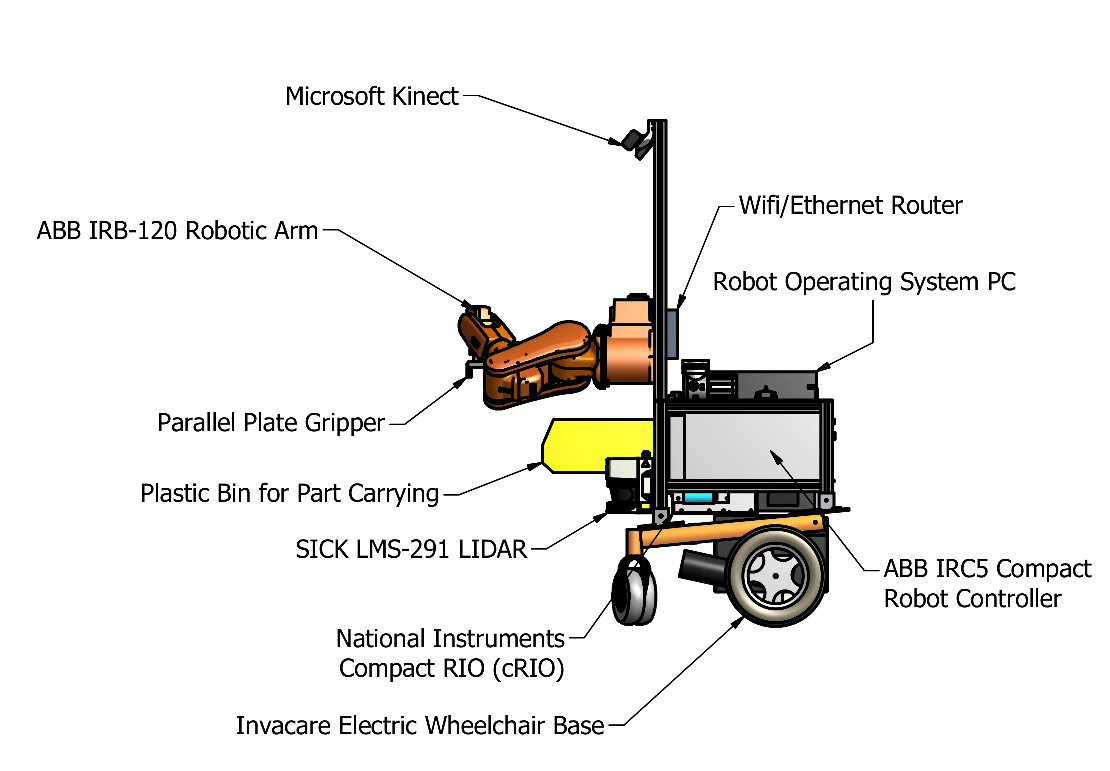
\includegraphics[width=6.0in]{abby-diagram}
\caption{An annotated rendering of ABBY showing several major components.}
\caption*{\textcopyright 2013 IEEE \cite{venator_case}}
\label{abby-diagram}
\end{figure}

\section{Invacare Ranger Wheelchair Base}

The Invacare Ranger is a wheelchair chassis in Invacare's Storm series.
The wheelchair base has a differential drive system with two pneumatic
drive wheels in the back and two solid caster wheels in the front. The
drive wheels are each powered by a 24 volt DC motor geared for a maximum
speed of 5 miles per hour (2.24 m/sec) \cite{venator_case}. Because of the
configuration of the robot's wheels, it can spin on its own axis and
drive forward and backward. It cannot move sideways.

The Invacare motor control electronics have been replaced with a
Sabertooth 2x50 dual brushed DC motor controller. The Sabertooth 2x50 is
an H-bridge PWM motor controller that supplies a variable DC voltage
from -24 volts to +24 volts to each motor based on commands it receives
over a serial data connection. The Sabertooth 2x50 is powered by a 24
volt DC rail that is energized and de-energized by the emergency stop
circuit described in Section \ref{estop}.

The wheelchair base is prone to wheel slip when commanded to accelerate
or decelerate quickly. The acceleration limits of the robot were
characterized by testing a series of constant linear acceleration
commands. These tests were performed with the robot's arm in the stowed
position on a smooth tile floor. From these tests, the maximum
achievable forward acceleration (with no slip) was determined to be
about .1 m/sec\textsuperscript{2} on tile floor. The same test was
performed using constant rotational accelerations. From these tests, the
maximum rotational acceleration was determined to be about 0.1
rad/sec\textsuperscript{2} on tile floor.

\section{ABB IRB-120 Robotic Arm}

The manipulator on the robot is an ABB IRB-120 industrial robotic
arm \cite{abb}. The IRB-120 is a six-axis robotic arm with a spherical
wrist. It has a tool flange that allows for the mounting of end
effectors as well as pneumatic and electrical connections near the tool
flange to connect sensors and actuators to the arm. The IRB-120 is ABB's
smallest robotic arm, with a 580 mm reach and a payload capacity of 3
kg. The arm itself weighs 25 kg and is mounted to the extreme front of
the robot, which means its weight exerts a large moment on the robot.
This was a serious consideration in the placement of the robot's center
of mass. The arm can be mounted at any angle, and on this robot is
mounted at 90° (with the base mounted to a vertical surface). The arm is
mounted vertically on the front of the robot so that the majority of the
arm's work envelope is outside of the volume of the robot. This
maximizes the functional work envelope of the arm and minimizes the
possibility of the arm colliding with other parts of the robot. However,
this mounting orientation does somewhat hamper the arm's ability to lift
objects from horizontal surfaces.

The IRB-120's joints are powered by non-back-drivable AC electric
servos, with position feedback from resolvers. According to ABB, the
IRB-120 is capable of position repeatability of 10 micrometers \cite{abb}.
The arm's position is controlled by an ABB IRC5 Compact robot
controller, which is in turn commanded through the ROS Industrial
interface. The details of this control structure are described in Section
\ref{hardware-drivers}.

\section{End Effector}

There are many types of grippers and graspers used with industrial
robots. Some are purpose-built fixtures for holding specific parts.
Other grippers use suction to be able to quickly pick up light objects
such as electronic components. Still others use dexterous fingers to be
able to securely pick up and manipulate objects of different shapes and
sizes. This robot uses one of the simplest gripper types, a two-position
parallel plate gripper.

The gripper was primarily chosen based on cost and availability. A
dexterous grasper like the BarrettHand costs about \$30k, which would
nearly double the cost of this robot. The pneumatically-actuated
parallel plate gripper has only two positions (open and closed), and is
simply and cheaply constructed from aluminum and a single double-throw
pneumatic piston. When open, the gap between the jaws is 53 millimeters,
and when closed the gap is 35 millimeters. The insides of the jaws are
lined with high-friction conveyor belt material.

The gripper is pneumatically actuated using stored air from accumulator
tanks that are kept at 825 kPa by an onboard compressor. The compressor
is turned on and off by an Innovation First Spike relay, which is
controlled by a digital pressure switch calibrated to turn the
compressor on at 690 kPa and turn it off at 825 kPa. This control
circuit can be seen in the power distribution diagram in 
Figure \ref{fig:power-schematic}. The 825 kPa stored air is regulated down to 
275 kPa working pressure and used to actuate the gripper. The pneumatic piston 
in the gripper is controlled by a pneumatic solenoid valve, a magnetically 
actuated valve with one pressure inlet and two pressure outlets. The inlet is 
connected to the regulator, and the outlets are connected to the gripper's
pneumatic piston so that applying pressure through one outlet opens the
gripper and applying pressure through the other outlet closes the
gripper. The solenoid valve is designed to that when one outlet is
connected to the pneumatic pressure inlet, the other is vented to the
atmosphere. The valve is actuated by running current through a solenoid
coil. The solenoid coil is controlled by a custom circuit based on an
Arduino microprocessor development kit, as shown in Figure 
\ref{fig:gripper-schematic}.

\begin{figure}[ht]
\centering
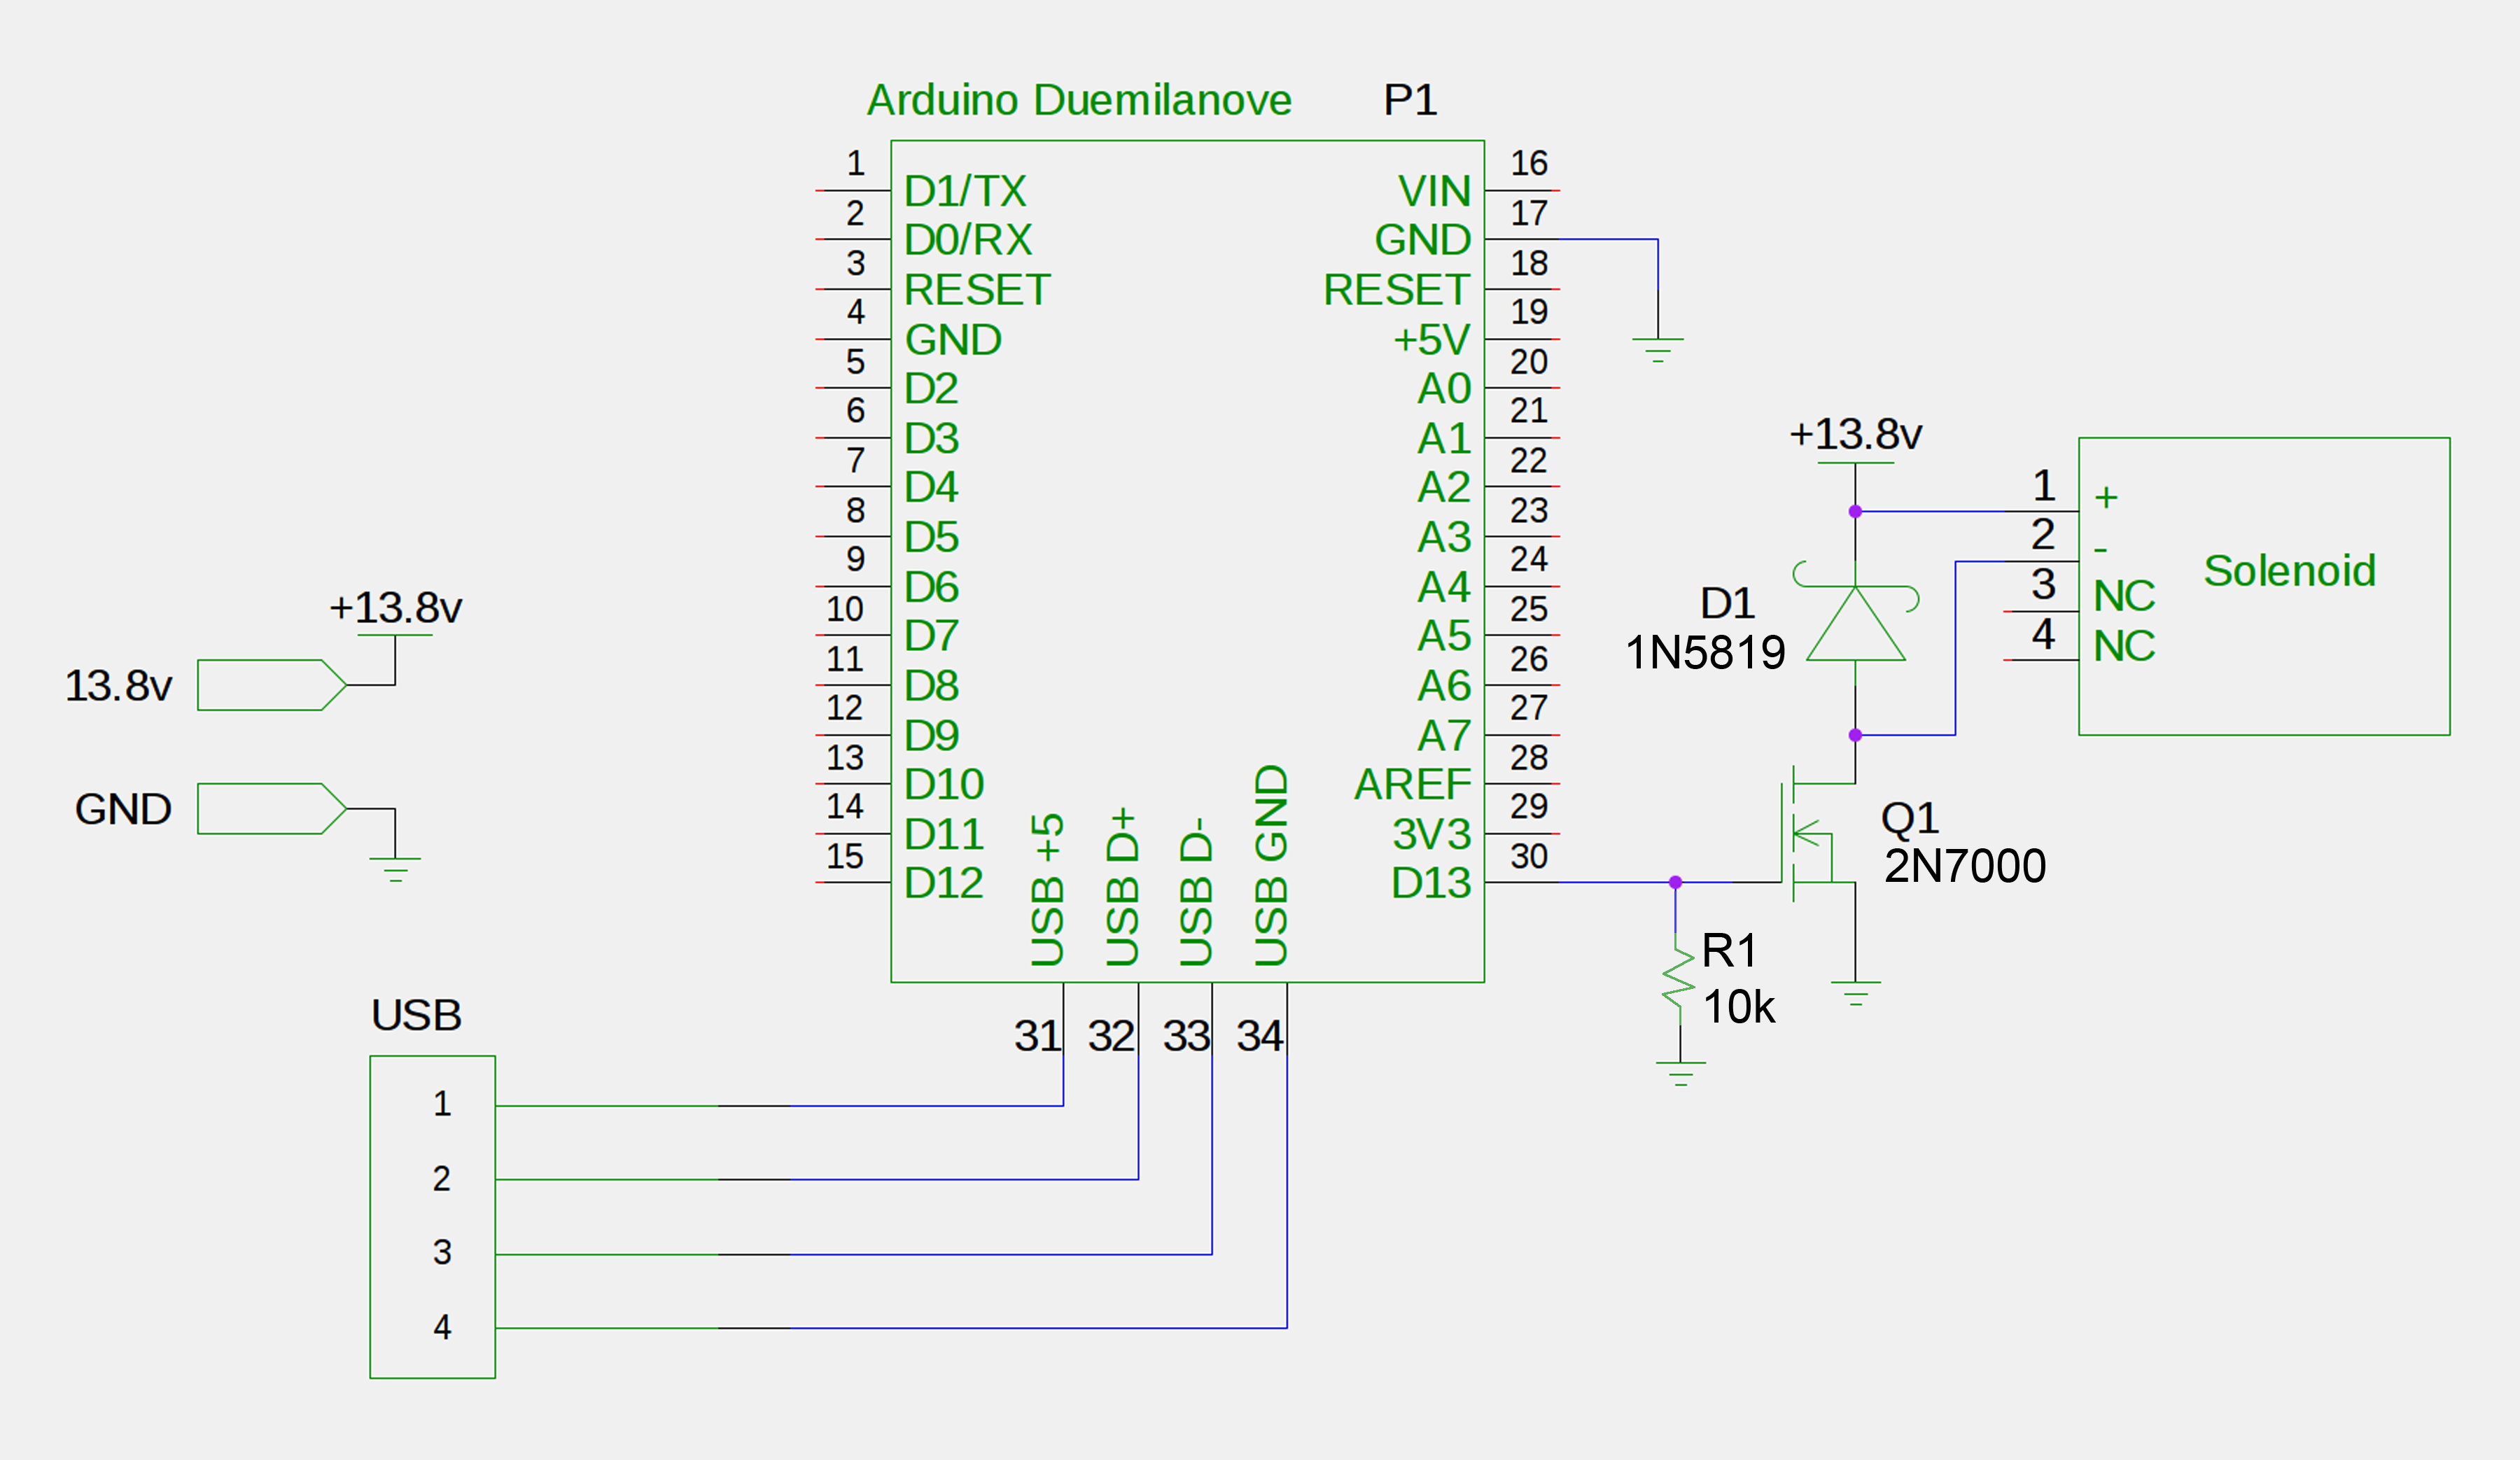
\includegraphics[width=6.0in]{gripper}
\caption{The electrical circuit to control the pneumatic gripper using 
an Arduino microcontroller and a pneumatic solenoid valve.}
\label{fig:gripper-schematic}
\end{figure}

Although the gripper has only two positions, the pneumatic nature of the
system makes the gripper jaws back-drivable, with a constant gripping
force proportional to the working pressure of the pneumatic system,
which was set by the pneumatic system's adjustable regulator to 275 kPa.
The regulator can be set to any pressure up to the system's maximum
pressure of 825 kPa. The working pressure was chosen so that the
gripping force would be great enough to ensure a strong grasp on
manipulated objects without being so great as to damage
them.

\section{Custom Frame Design}

Coupling together the ABB IRB-120 robotic arm and the Invacare Ranger
wheelchair base is the main frame of the robot. The structural elements
of the frame are made from Bosch Rexroth aluminum profile struts. Bosch
rail is an extruded aluminum product with T-slots running the length of
the rail. It has several features that make it a good choice for a
prototype robot. Because Bosch rail is aluminum, it is easy to machine,
but strong and relatively light. Because T-slots do not require holes to
be drilled in the rail for mounting, the robot can be easily
reconfigured without remachining frame members. However, heavy objects
mounted to vertical rails, such as the arm, may slip if the bolts are
not very tight.

\begin{figure}[ht]
\centering
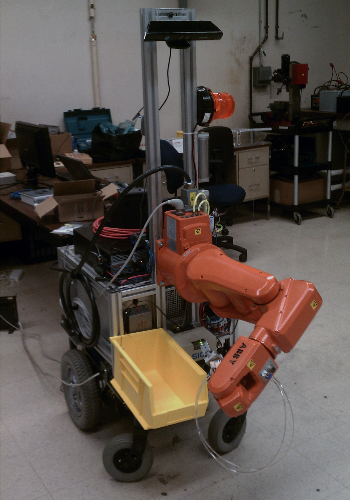
\includegraphics[height=5.0in]{abby_2_edited}
\caption{ABBY, a mobile industrial manipulator.}
\caption*{\textcopyright 2013 IEEE \cite{venator_case}}
\label{fig:abby-photo}
\end{figure}

The frame is designed to hold the IRC5 Compact robot controller and the
assorted power and control electronics of the robot. The IRC5 is large
(480mm x 580mm x 258mm) and heavy (28.5kg), and it dominates the robot
frame. The robot frame was meticulously designed in 3D CAD software to
place the center of mass as close to the center of the robot volume as
possible to prevent tipping. The mass of every component of the robot
was entered into the CAD models, and components were placed so as to
keep the center of mass low as well as relatively centered between the
front and rear wheels. The final center of mass, as determined by the
CAD model, is 0.2 meters in front of the rear wheels (0.48 meters behind
the front wheels) and 0.494 meters from the ground. The robot's
estimated weight is 195 kg.

On the front of the frame is a vertical mast made of Bosch rail. This
mast serves several purposes. First and foremost, it provides a mounting
point for the IRB-120 robotic arm. The rails are spaced so that the
arm's four mounting holes line up with the two rails, and the arm can be
fixed to any position along the height of the rail by tightening the T
nuts that hold it in place. This allows the robot to be reconfigured for
different tasks that may require the arm to be mounted at different
heights. In addition to holding the arm, the mast provides a high
vantage point for the Kinect camera and allows the WiFi router to be
mounted far away from possible interference from other electronics.

In addition to the Bosch rail structural elements, the frame includes
four panels for mounting the robot's electronic and pneumatic
components. It was important to protect the onboard electronics from
damage in the case of a collision, so the majority of the electronics
are mounted to a polycarbonate panel underneath the IRC5, where they are
completely enclosed inside the robot. This keeps the electronics safe
from collisions, and the mass of the heavy power electronics is kept low
to the ground. Although this design is advantageous in terms of keeping
the robot's overall volume small and the robot's center of mass low, it
is not user-friendly in the rare event that these components require
service.

The top panel of the robot, also made of polycarbonate, holds the
pneumatic system and the PC. These were mounted on the top panel in
anticipation that they would require more user access and to put the
pneumatics close to the arm. Two front panels, made of aluminum sheet,
hold the main power distribution rail and the power supply for the
LIDAR. The power distribution rail is mounted on a front panel to make
it easily accessible, and the LIDAR power supply is mounted on a front
panel to place it close to the LIDAR, which is mounted to the front
frame rail.

\section{Power}

\begin{figure}[ht]
\centering
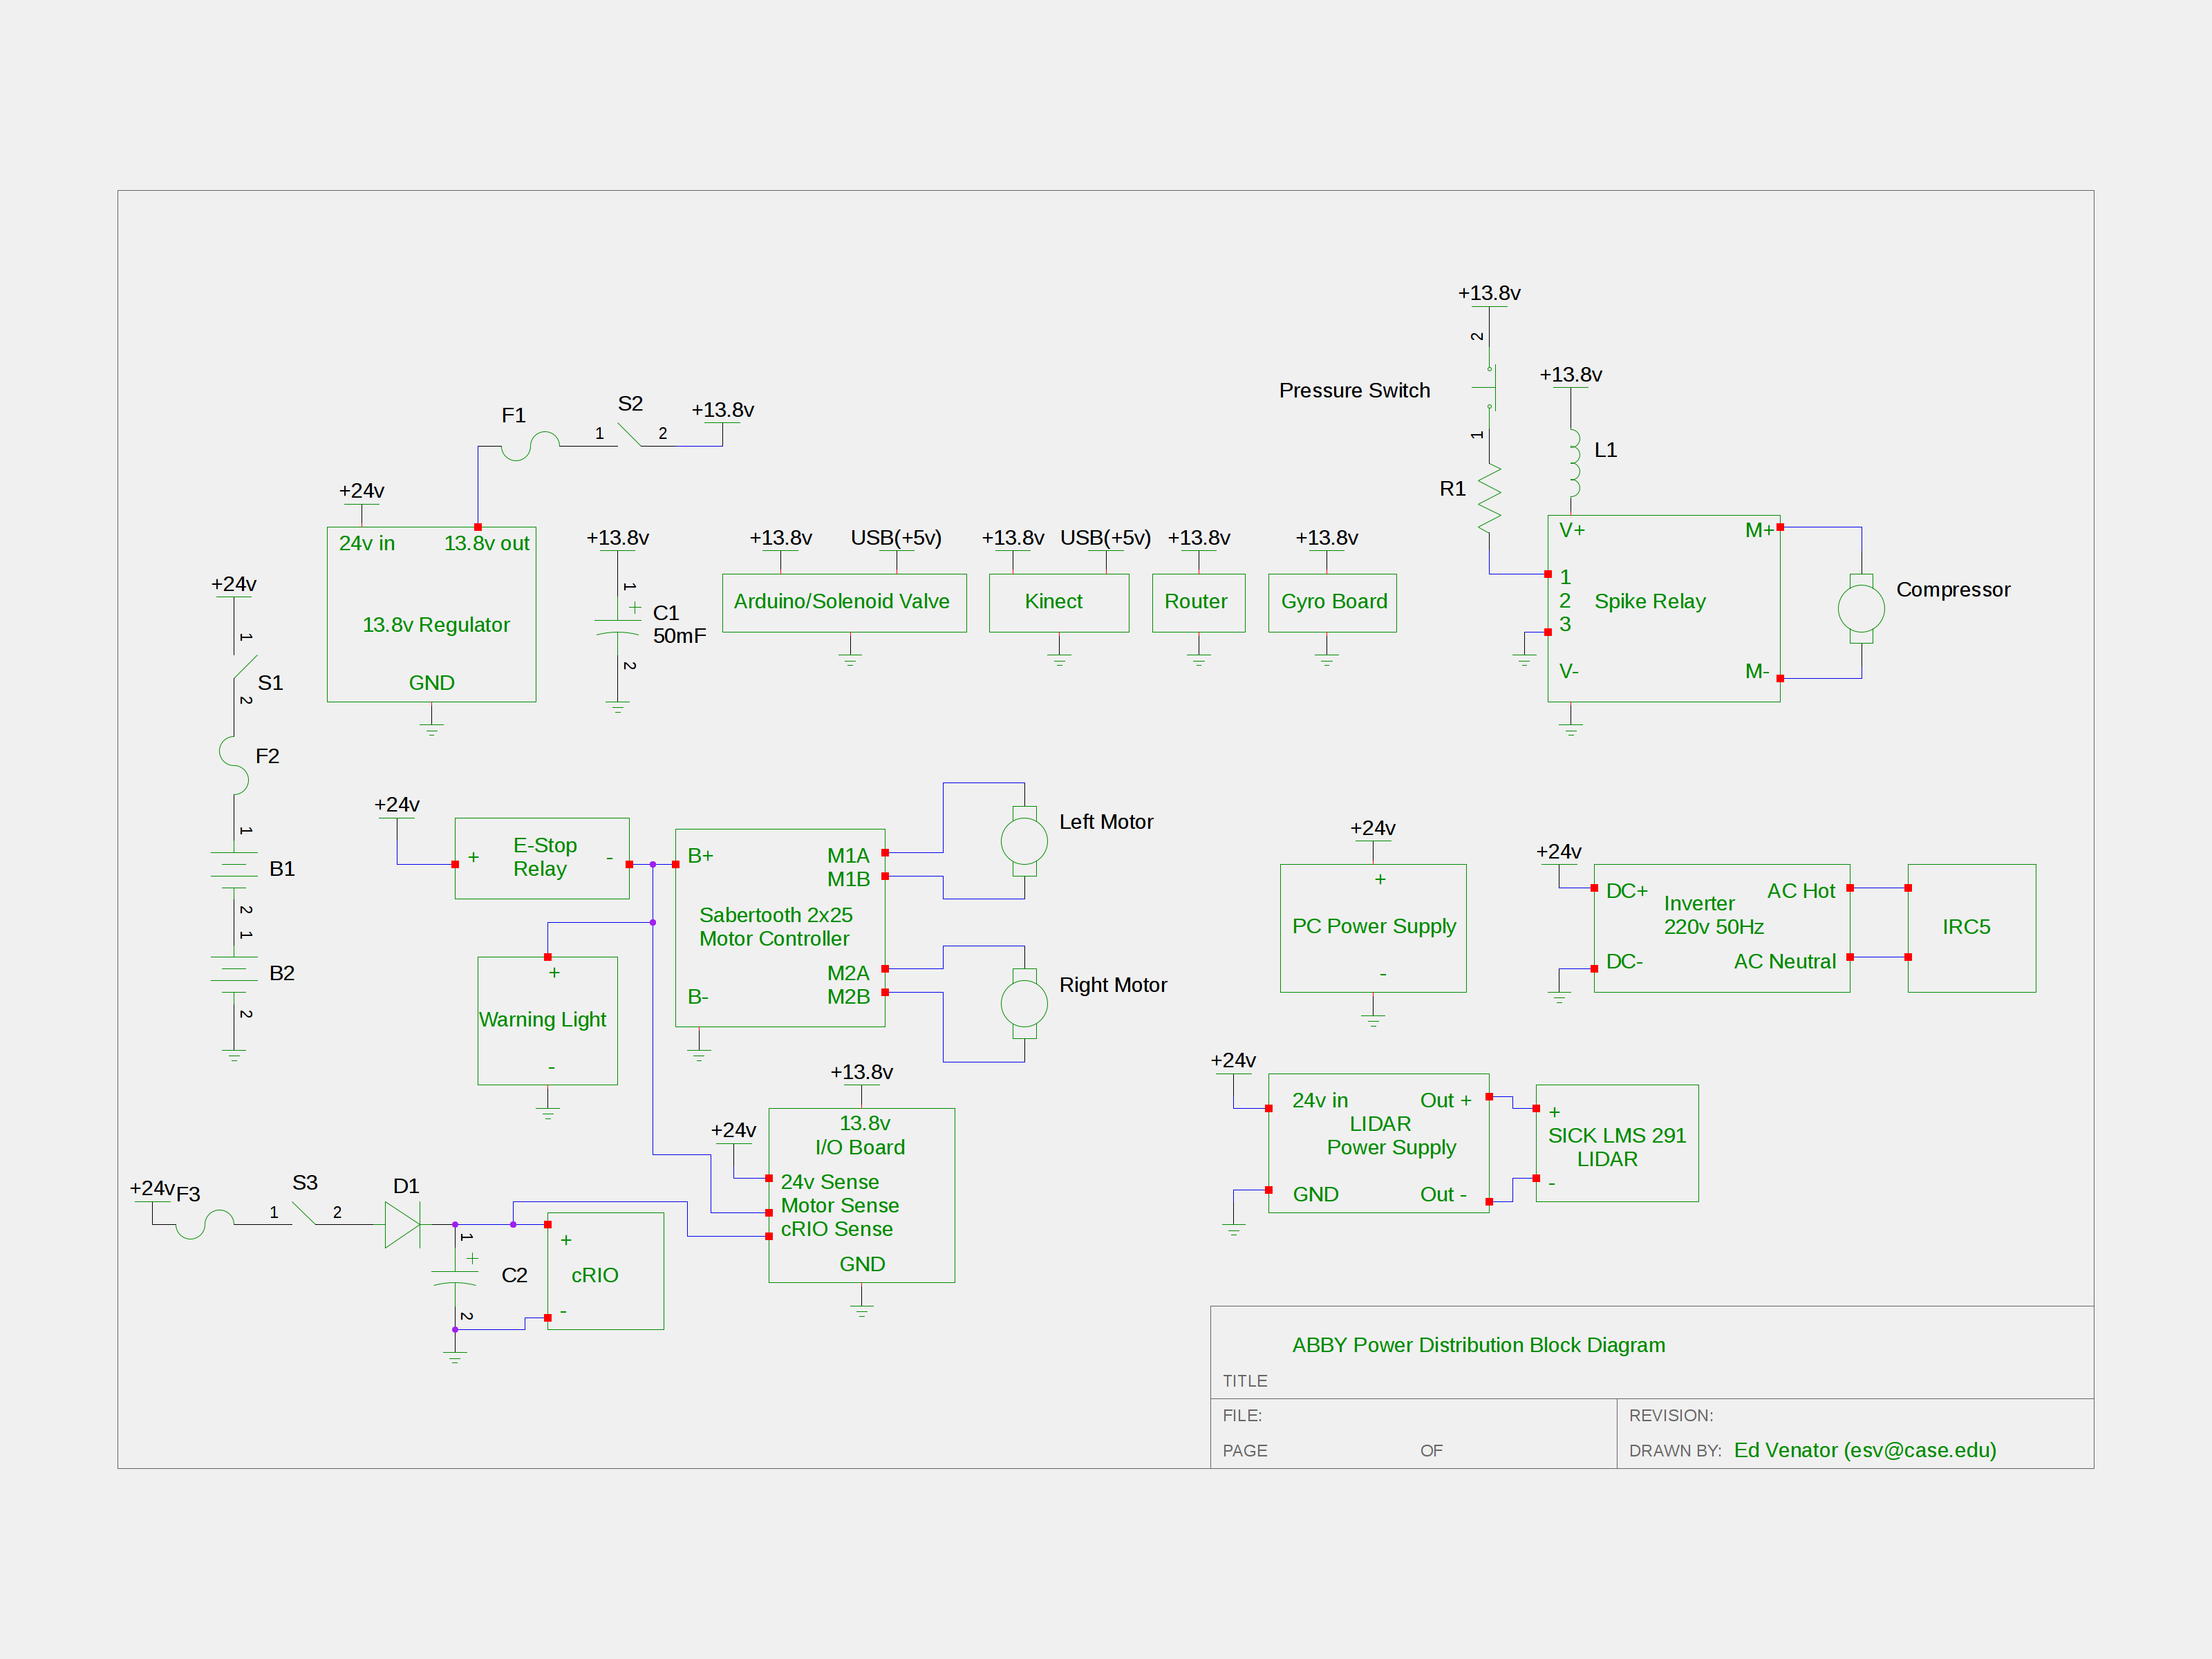
\includegraphics[width=6.0in]{power_block_diagram}
\caption{A block diagram of the power distribution system on the robot}
\label{fig:power-schematic}
\end{figure}

All of the robot's power is distributed using DIN rail power
distribution blocks. These blocks are modular, insulated, and compact.
The robot has two DC voltage buses (24 volt DC, and 13.8 volt DC) and a
single ground block. In addition to these main voltage buses, several
parts of the robot have their own power regulators and supplies.

The robot's main voltage rail is a 24 volt DC bus supplied by two 12
volt batteries in series. This 24 volt bus is required by the Invacare
wheelchair base's drive system, and the Invacare wheelchair base
includes the batteries that supply the bus. The batteries are protected
by a 120 amp resettable circuit breaker, which also serves as the main
power switch for the robot. In addition to the robot's drivetrain, the
robot's PC, LIDAR, and the National Instruments cRIO are all powered
directly from the 24 volt DC bus.

Because the cRIO is a critical component of the drivetrain and the
inductive kick of the motors can cause significant noise on the 24 volt
DC bus, a peak-detector circuit is used to protect the cRIO from voltage
fluctuations on the 24 volt rail.

In addition to the two DC buses on the robot, there is an AC inverter,
which is used to power the ABB IRC5 Compact robot controller. The IRC5
requires 220 volt AC at 50 Hz. The inverter is capable of delivering up
to 2 kW of power continuously and surges of up to 3kW, which is
necessary to account for the high current draw when the controller first
enables the motor drive. The inverter is powered from the 24 volt DC bus
and is only used to power the IRC5 Compact and (through the IRC5) the
IRB-120 robotic arm.

Much of the electronics on the robot requires a lower voltage to
operate, nominally 12 volts DC. These electronics are powered by a
Samlex America SDC-15, a 13.8 volt switch-mode step-down regulator that
can supply up to 12 amps \cite{samlex}, which is powered from the main 24 volt
bus. This bus powers the WiFi router, emergency stop circuitry, the cRIO
interface board, the Kinect camera, and the pneumatic compressor.

\begin{figure}
\centering
\begin{minipage}{.5\textwidth}
  \centering
  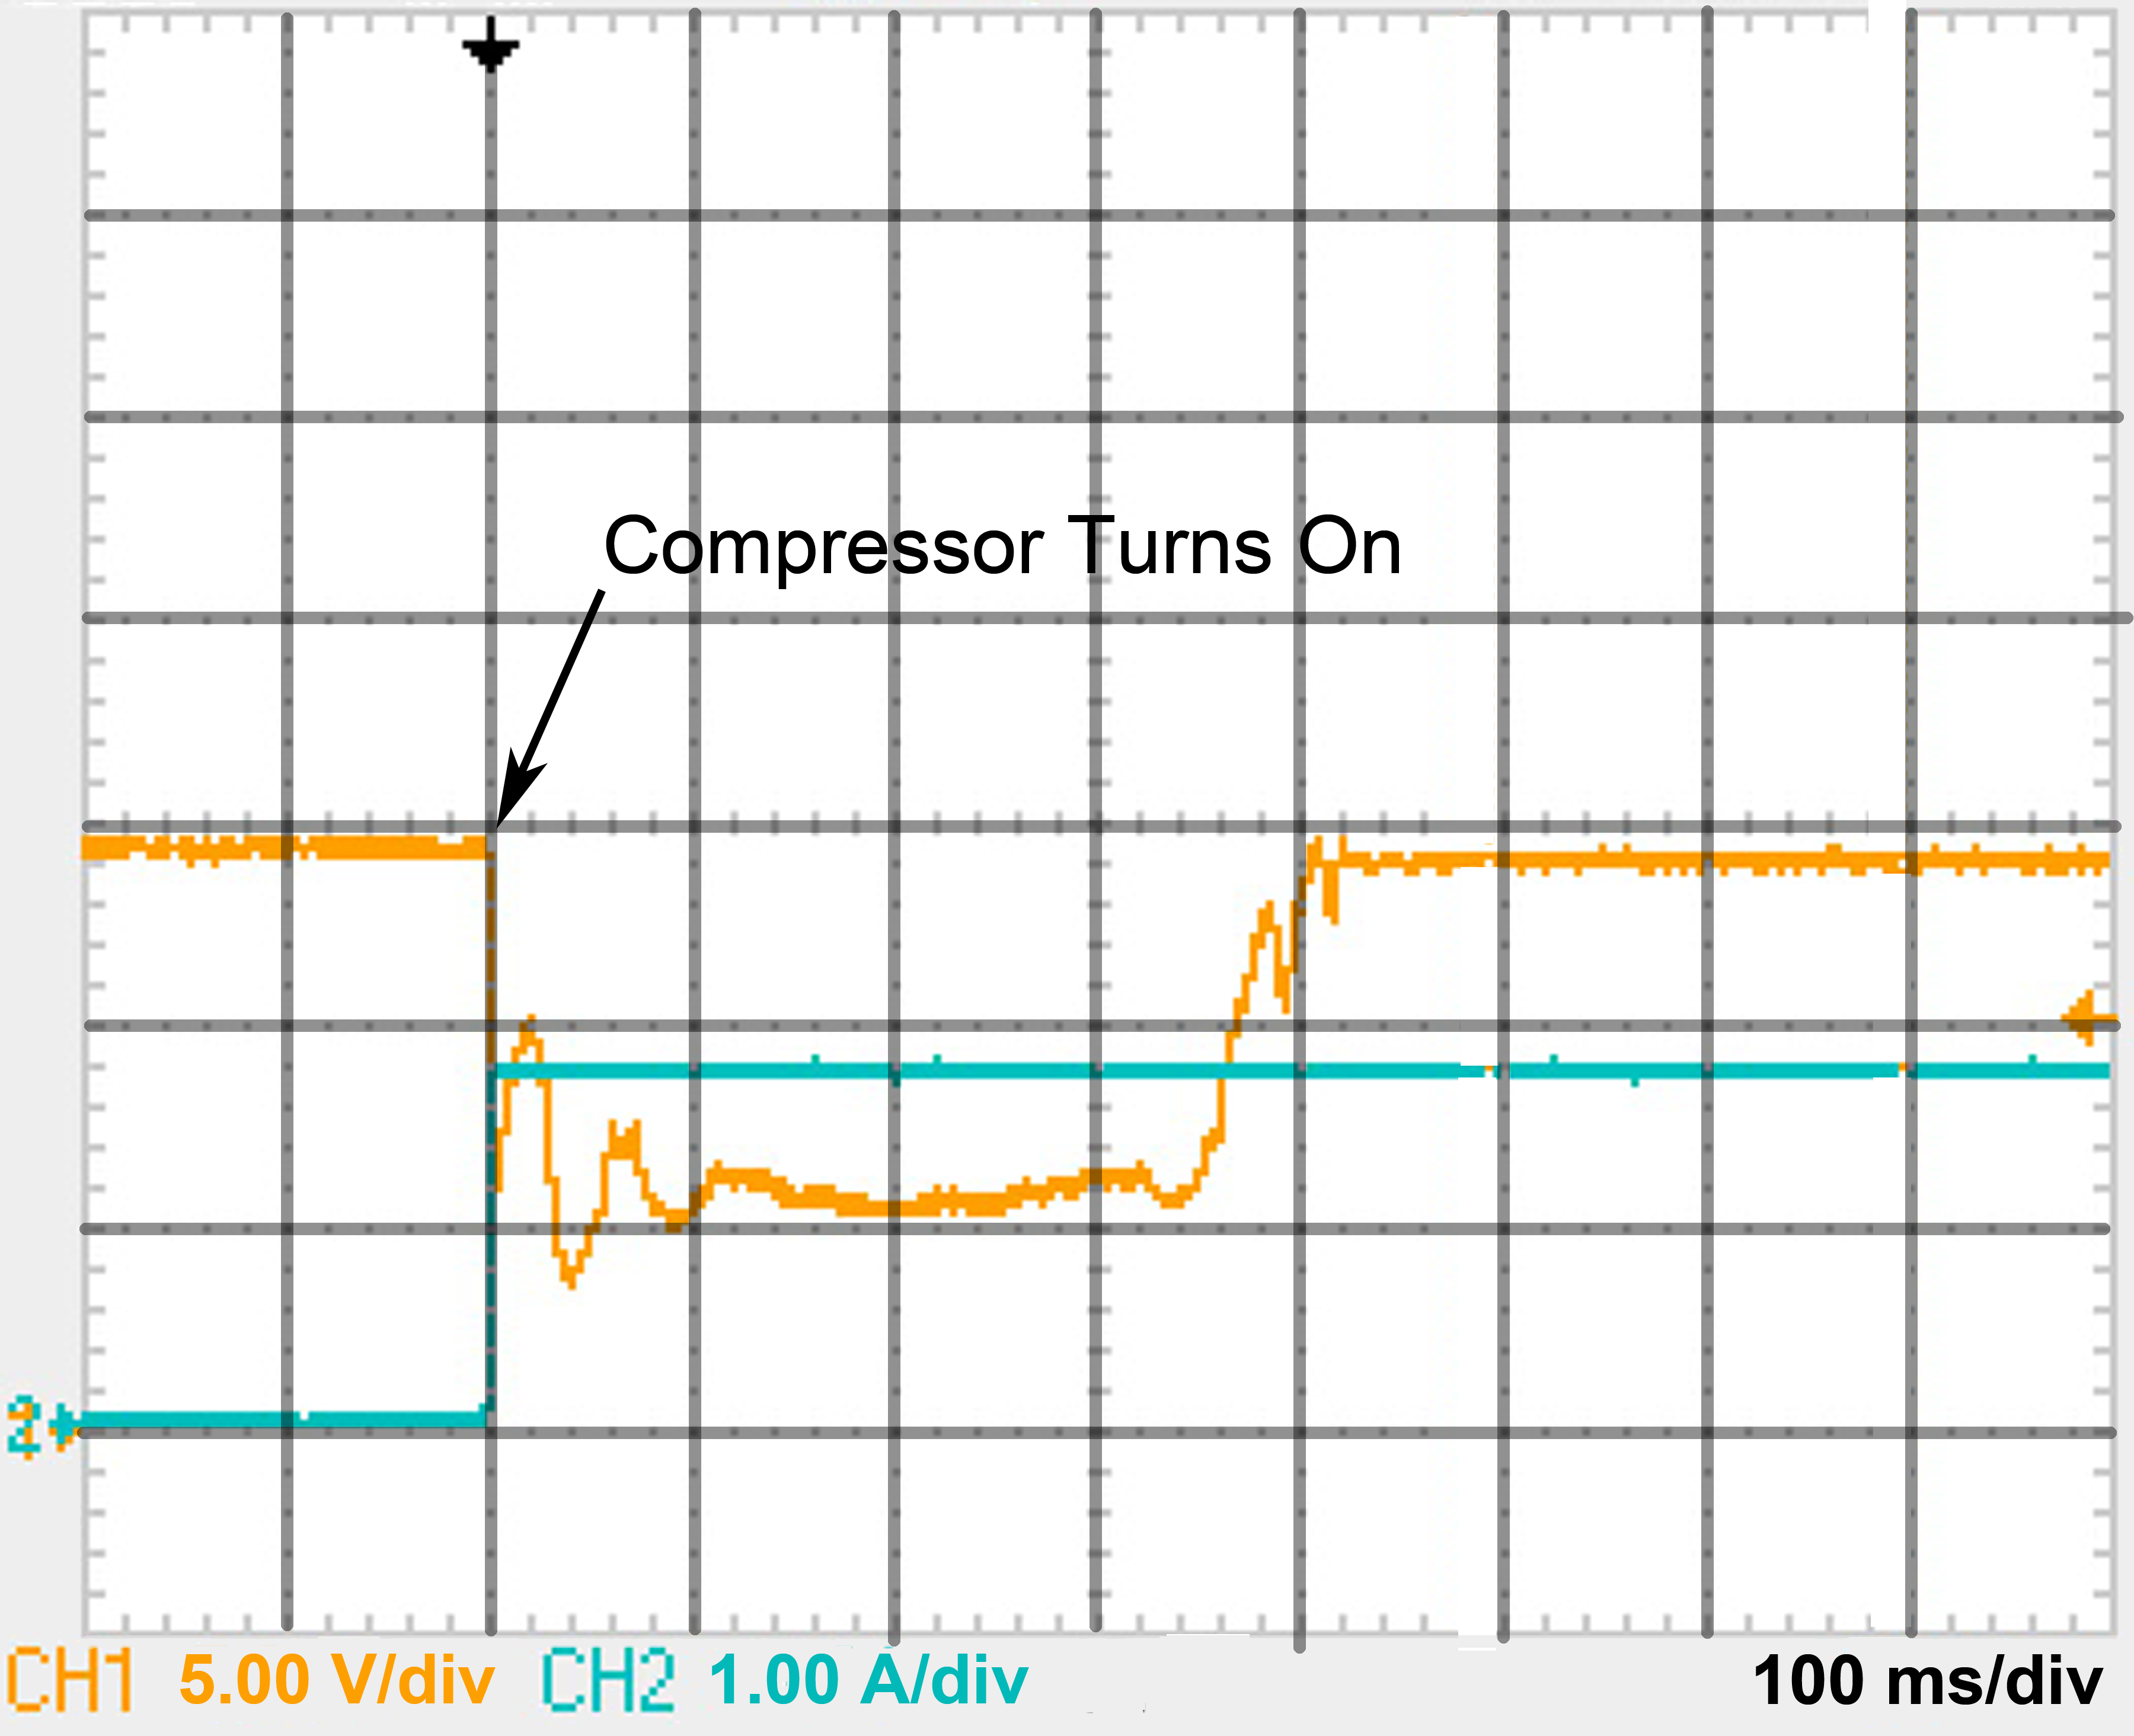
\includegraphics[width=.9\linewidth]{figure_5}
  \captionsetup{width=.9\linewidth}
  \captionof{figure}{13.8 volt rail dropout when compressor turns on (before addition of filter).}
  \label{fig:compressor-dropout}
\end{minipage}%
\begin{minipage}{.5\textwidth}
  \centering
  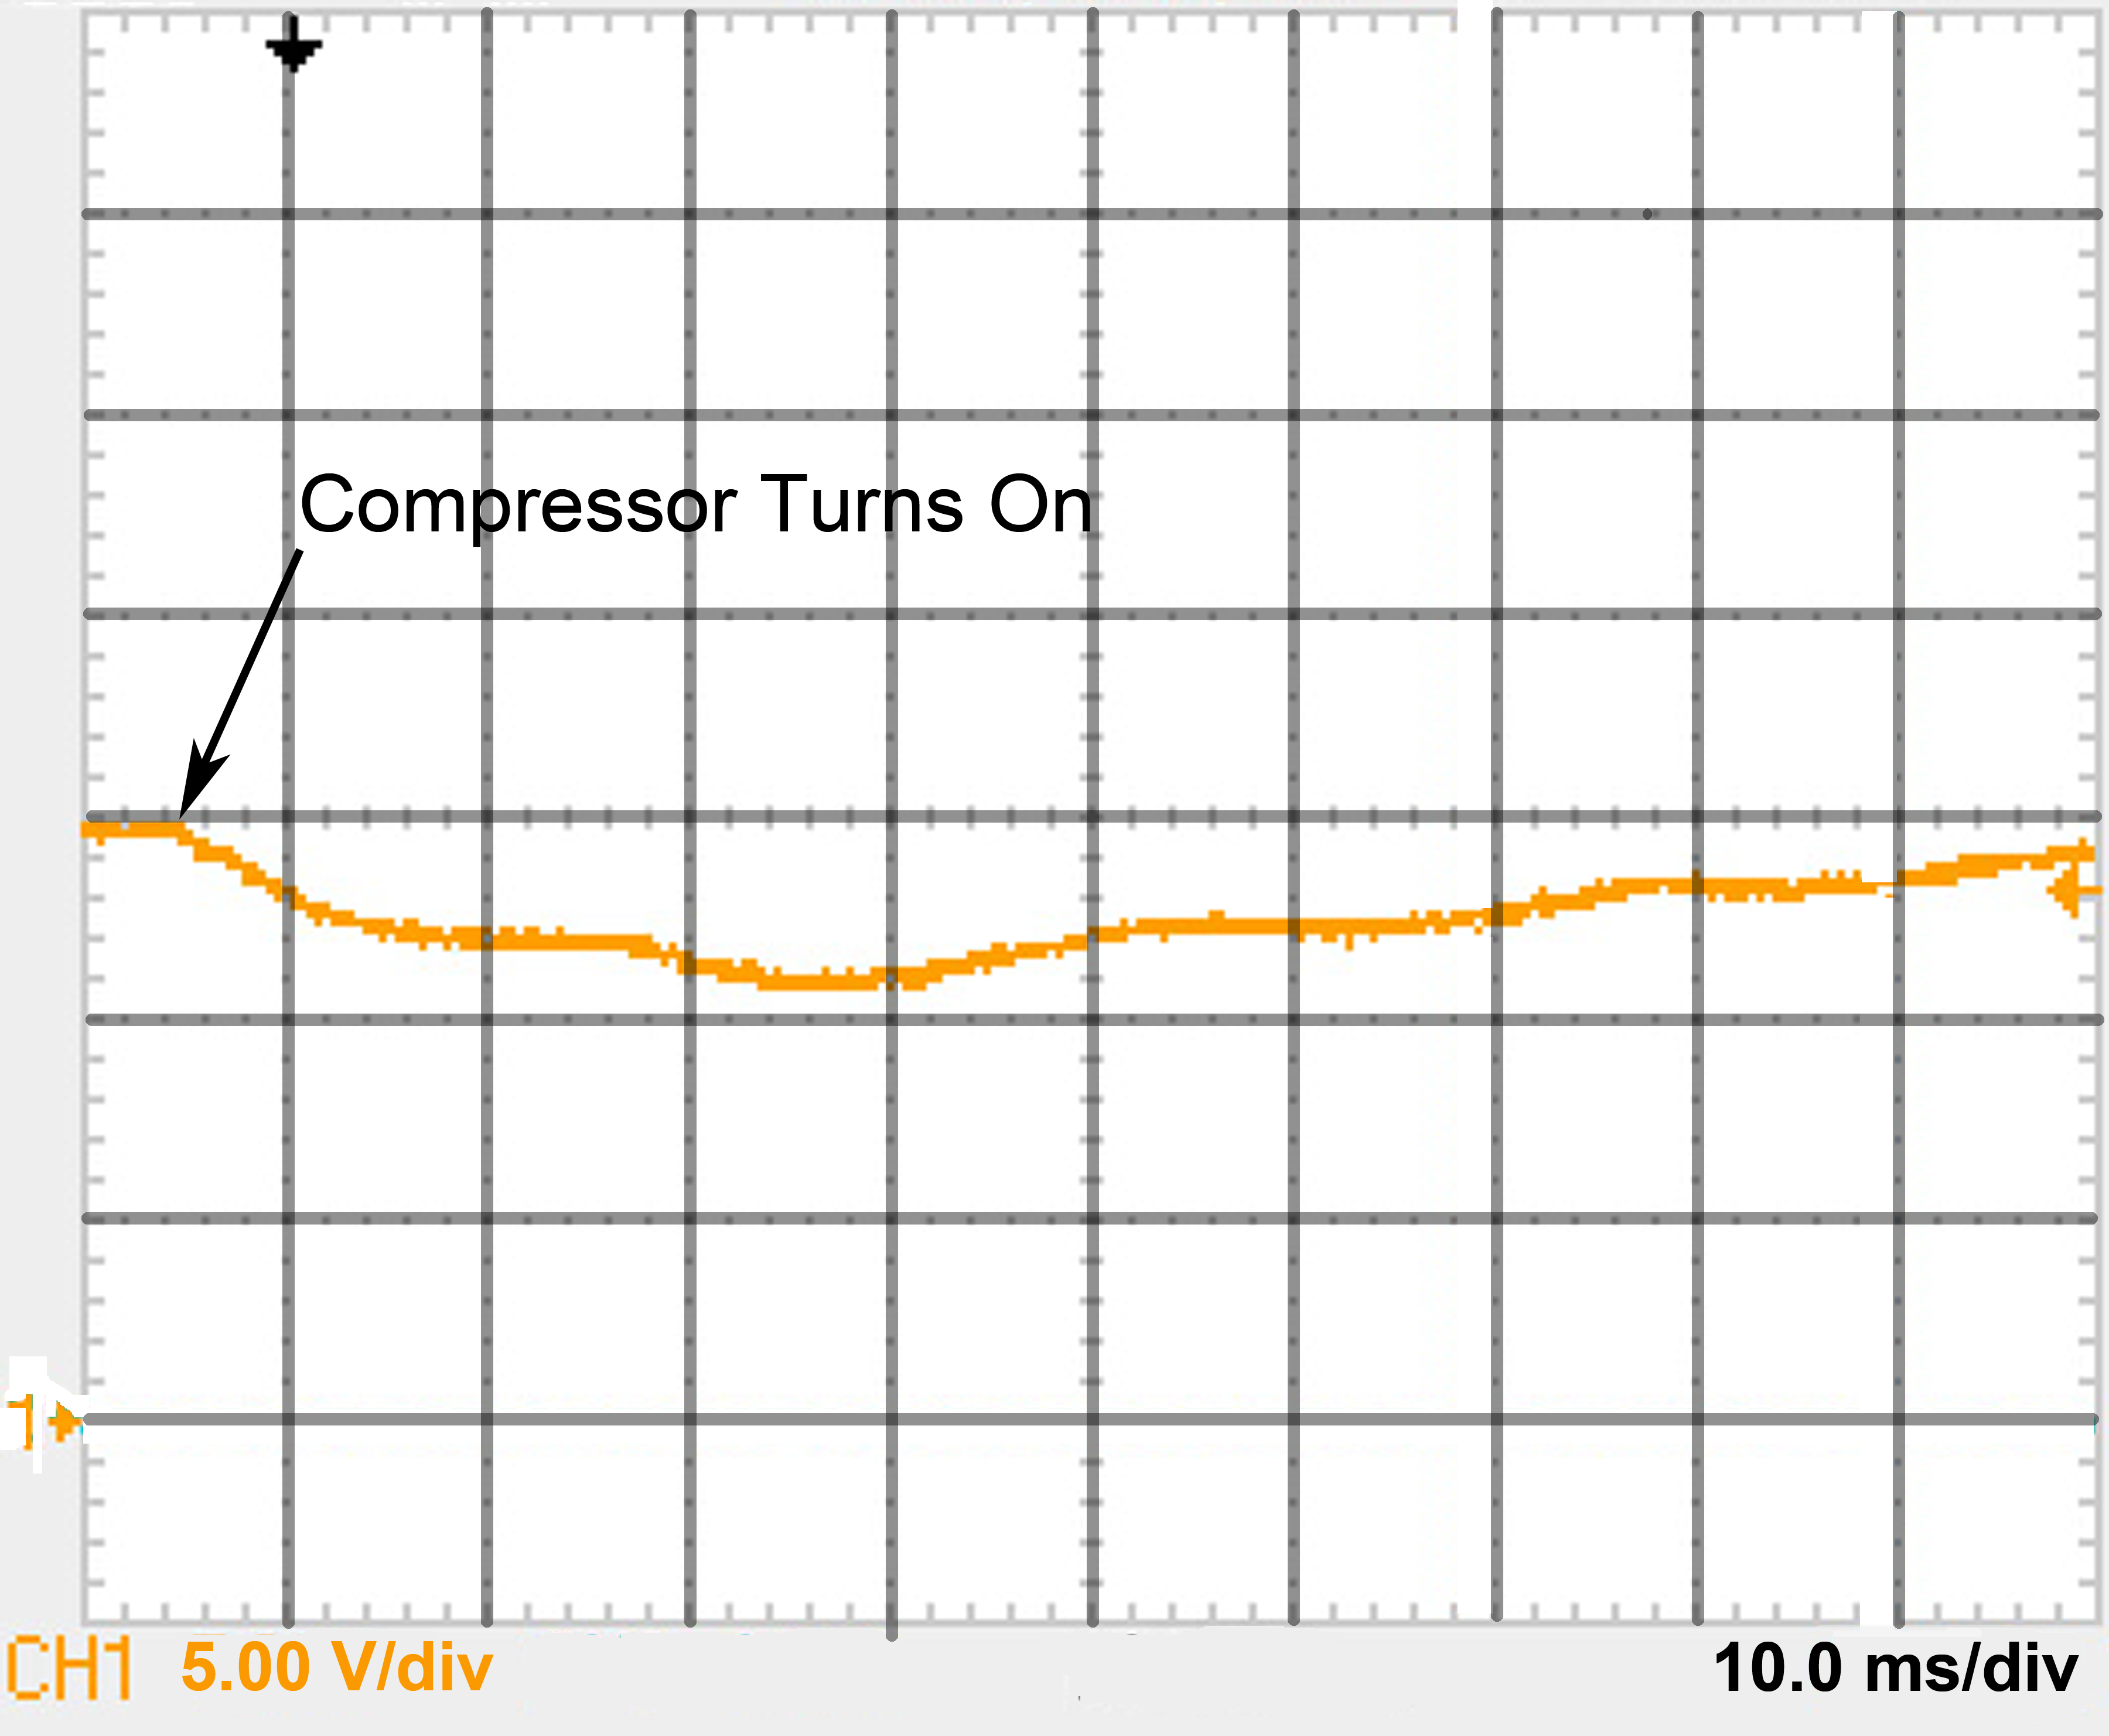
\includegraphics[width=.9\linewidth]{figure_6}
  \captionsetup{width=.9\linewidth}
  \captionof{figure}{13.8 volt rail during compressor turn-on after addition of an LC filter.}
  \label{fig:compressor-filter}
\end{minipage}
\end{figure}

Because the compressor draws a large amount of current, the 13.8 volt
regulator's output would drop to about 5 volts for approximately 450 ms
(see Figure \ref{fig:compressor-dropout}) when the compressor switched on. This droop was
sufficient to cause the onboard Ethernet router to reboot, interrupting
communications between the computers onboard. In order to prevent this
problem, an LC filter was added to the 13.8 volt power rail. A 50mF
capacitor acts as a charge reservoir for the electronics on the 13.8
volt power rail, including the router. A 55 μH inductor acts as a
current choke to limit the instantaneous current draw when the
compressor turns on. Figure \ref{fig:compressor-filter} shows that this filter kept the 13.8 volt
rail from dropping below 10 volts, and it recovers to its nominal
voltage in under 100 ms. This droop is not enough to cause the router to
reboot. In order to monitor the state of the voltage rails, each one is
connected to an analog to digital converter (ADC) on the National
Instruments Compact RIO that controls the drive base (see Section \ref{computing-hw}).
The ADC monitors the main 24 volt bus, the 13.8 volt bus, the power
supply to the cRIO (which is protected from rail droop by a peak
detector, as shown in Figure \ref{fig:power-schematic}), and the rail that powers the drive
base, which is switched on and off by the emergency stop circuit.

\begin{figure}[ht]
\centering
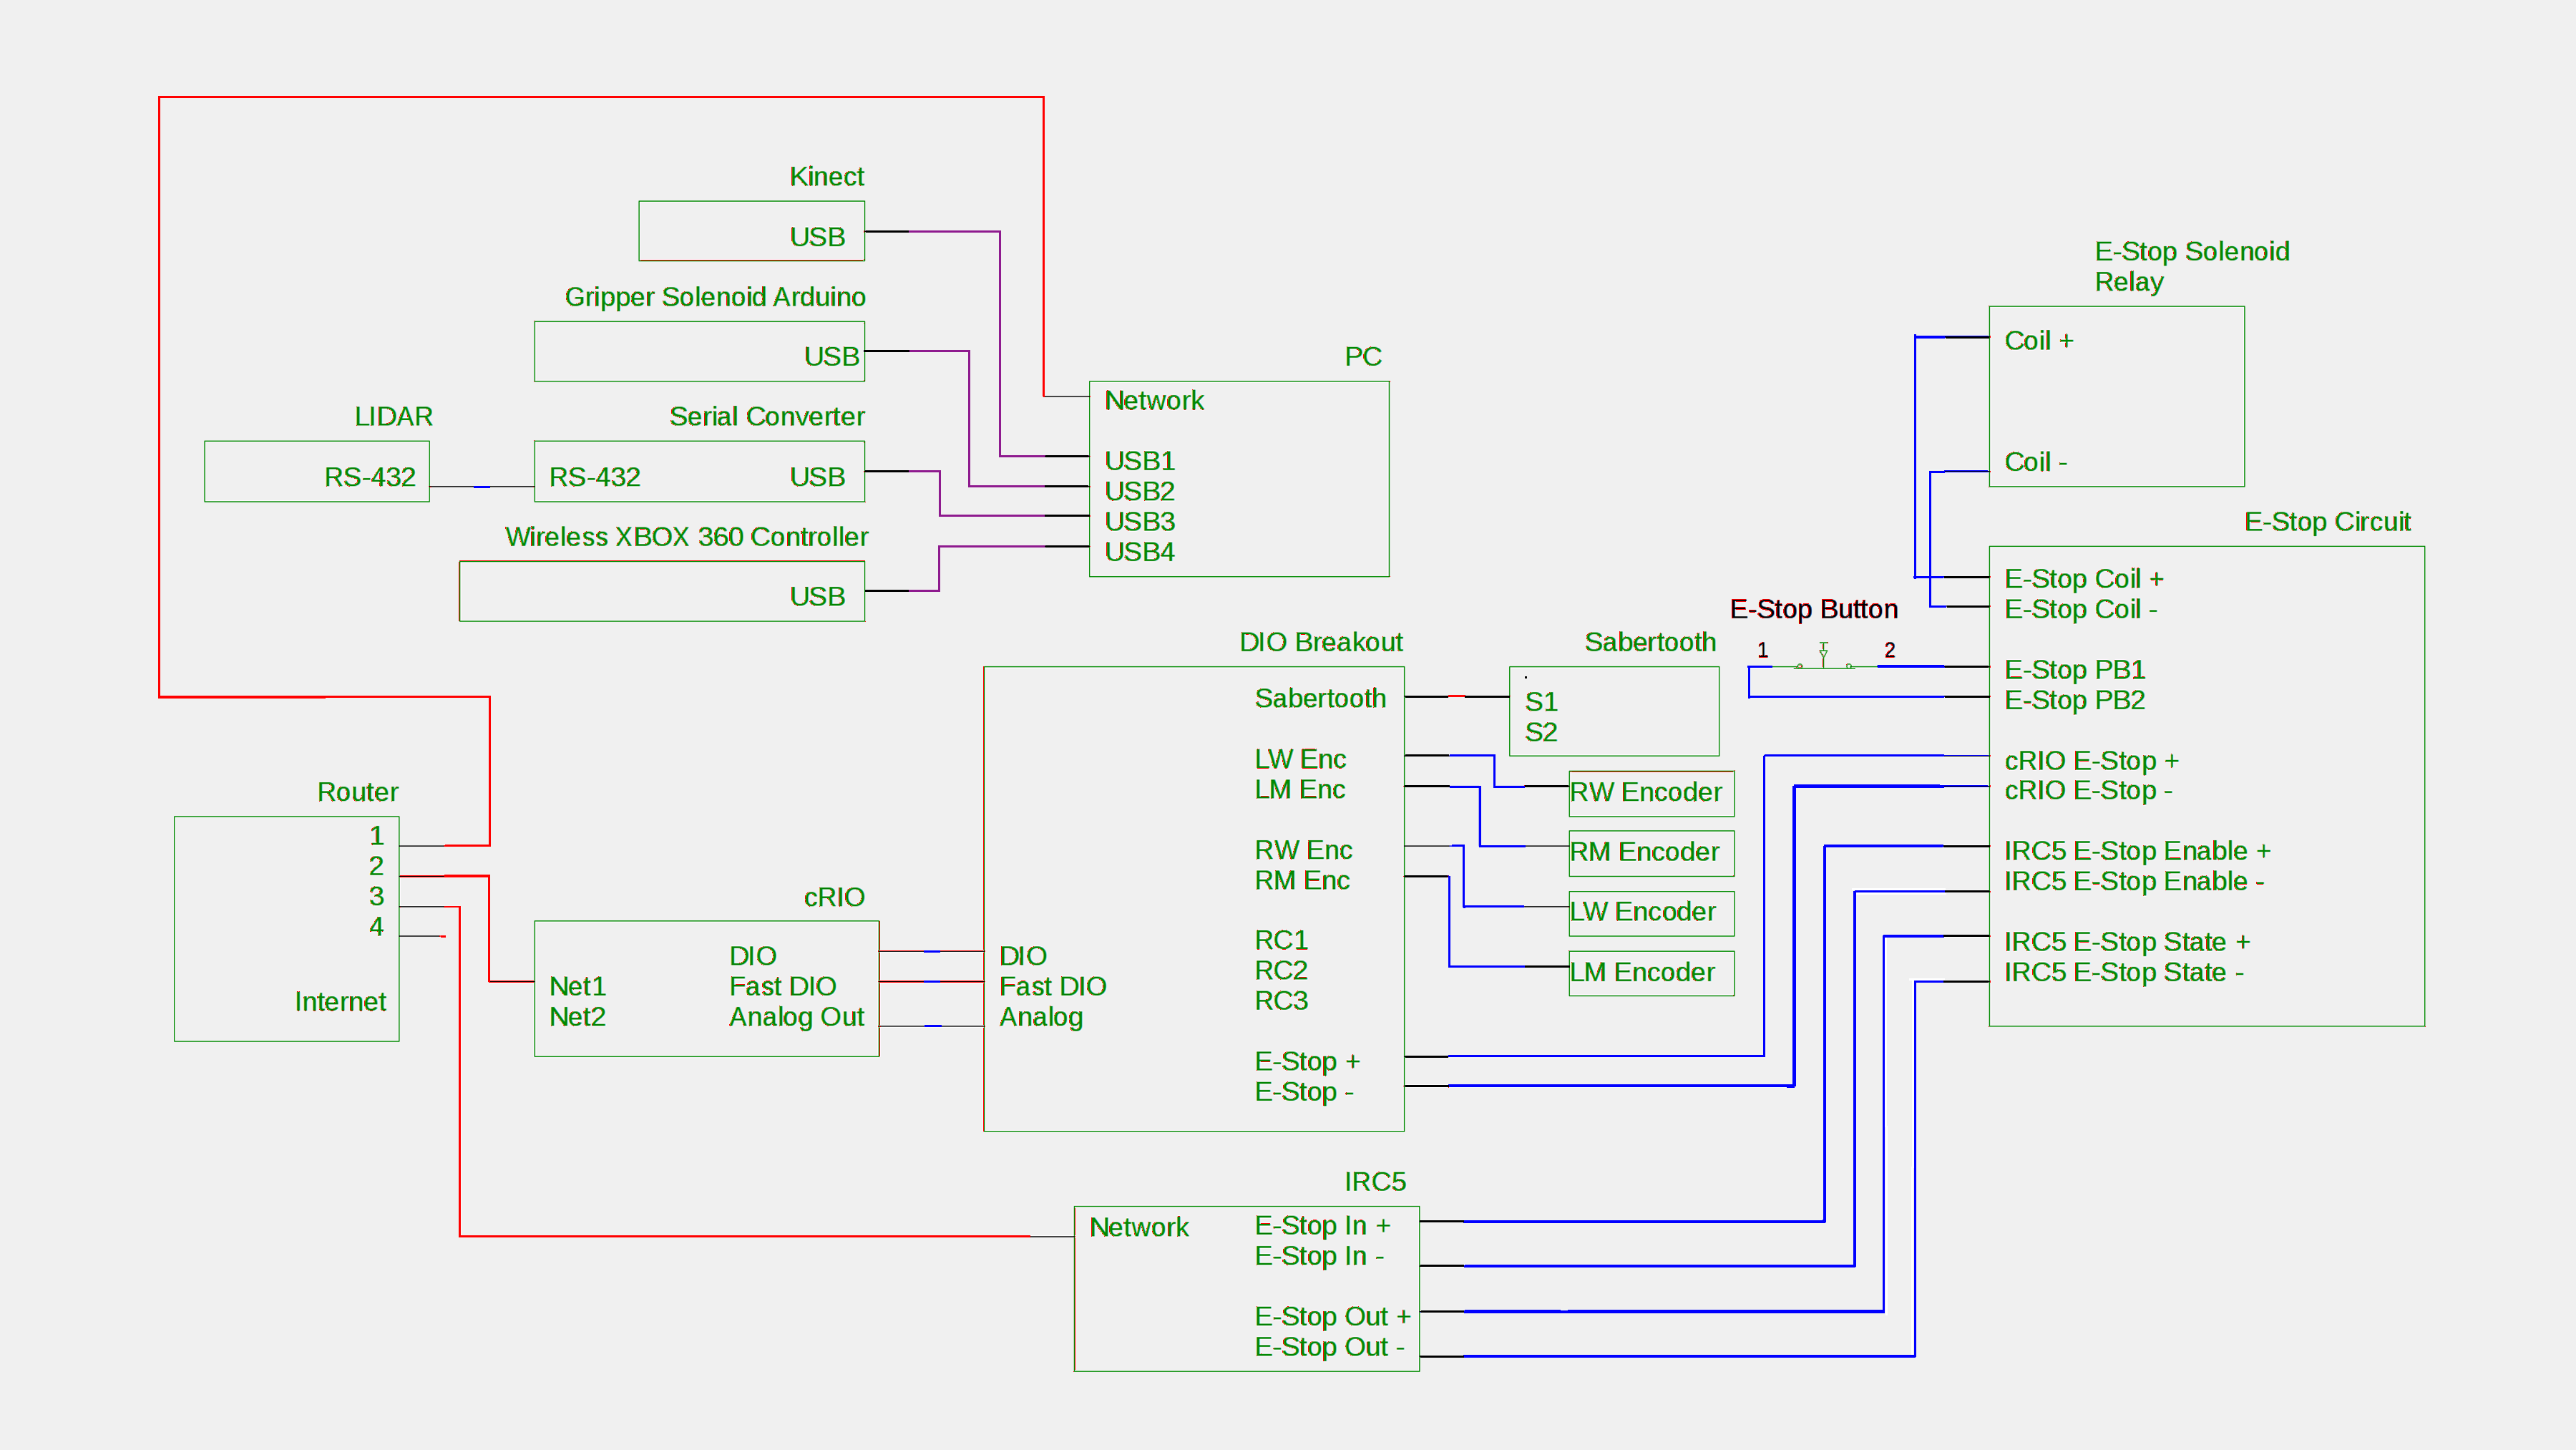
\includegraphics[width=6.0in]{data_block_diagram}
\caption{A block diagram of the sensors and computing hardware on ABBY, 
showing all data connections}
\label{fig:data-schematic}
\end{figure}

In order to sense the motor speed, there is a Grayhill 61R-256 encoder
on each motor's output shaft. The encoder outputs quadrature pulses at a
frequency proportional to the motor speed. These motor shaft encoders
cannot provide accurate wheel position information for odometry because
of backlash in the gearboxes. For odometry, there is an encoder attached
to each wheel by a toothed belt. The wheel encoders spin sixteen times
more slowly than the motor encoders, but still provide a very high
resolution output (0.7 mm per encoder tick). The output of the wheel
encoders is differentiated to get the wheel velocities, which are then
fed as control inputs into a Kalman filter that outputs a robot pose
estimate consisting of X and Y coordinates and a heading.

\begin{figure}
\centering
\begin{minipage}{.5\textwidth}
  \centering
  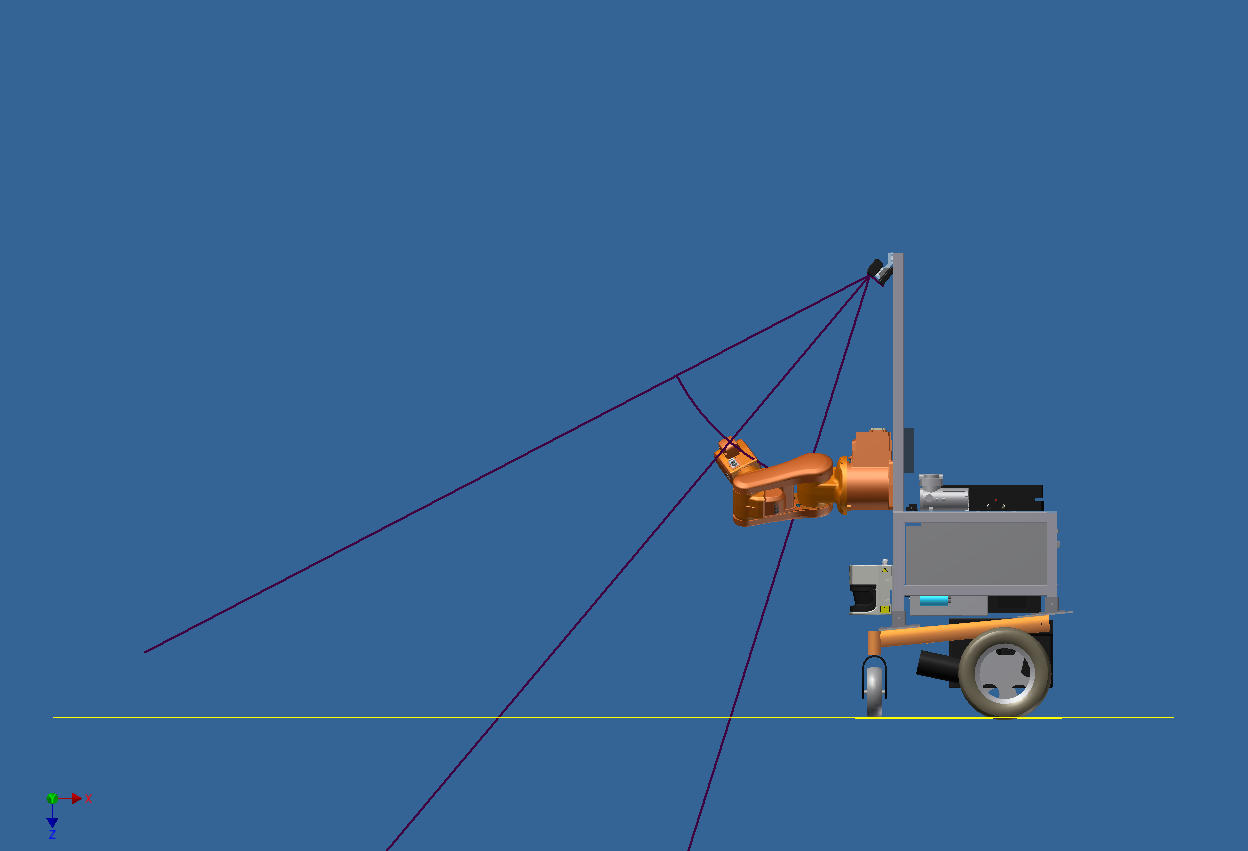
\includegraphics[width=.9\linewidth]{kinect_fov}
  \captionsetup{width=.9\linewidth}
  \captionof{figure}{A side view of the robot, showing the Kinect's field of view}
  \label{fig:kinext-fov}
\end{minipage}%
\begin{minipage}{.5\textwidth}
  \centering
  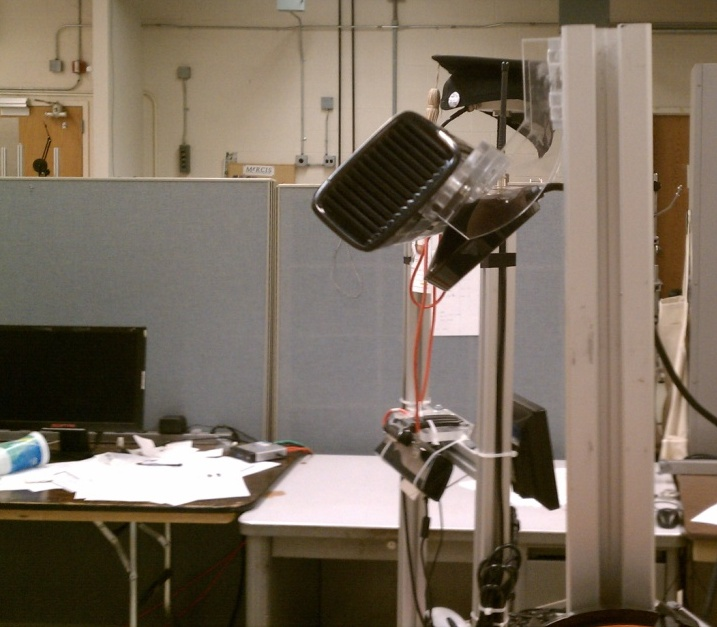
\includegraphics[width=.9\linewidth]{kinect_mount}
  \captionsetup{width=.9\linewidth}
  \captionof{figure}{A close-up view of the Kinect mounted to the robot, showing the mounting bracket}
  \label{fig:kinect-mount}
\end{minipage}
\end{figure}

The Microsoft Kinect is an RGBD (Red, Green, Blue, Depth) camera
marketed as a gaming controller. ABBY has a Kinect camera mounted high
on the front mast with a custom-designed acrylic bracket that fixes it
at a downward-looking angle of 51 degrees from the horizontal. At this
angle, the Kinect is looking down into the IRB-120's work envelope and
capable of viewing the floor in front of the robot. The RGBD data from
the Kinect are converted into three-dimensional point clouds, which are
used to detect obstacles and manipulable objects.

An LMS-291 laser ranging sensor (LIDAR) from SICK AG of Waldkirch,
Germany is mounted horizontally to the front of the robot. The LIDAR
provides planar range scans of a 180 degree arc in front of the robot.
These range data are used for localization and obstacle detection.

\section{Computing Hardware}
\label{computing-hw}

The robot has three main computing devices on board, connected by a
local Ethernet network with an onboard WiFi access point so operators
can wireless connect to the robot for maintenance and control.

The majority of the robot's processing is performed on a Linux PC. This
PC runs all of the perception and higher level planning algorithms,
which do not require a real-time operating system. In addition, the PC
is responsible for processing LIDAR and Kinect data directly from the
sensors. These tasks are computationally intensive, particularly the
tasks of filtering the robot's links out of the Kinect point cloud and
maintaining a collision map.

The computer was specified so as to balance cost, physical size, and
processing power. The computer's motherboard is an ASUS micro-ATX
motherboard, which was chosen over the smaller mini-ITX form factor
because many mini-ITX boards were found to have poor thermal management
during the construction of the autonomous wheelchair OTTO. The case
chosen was the smallest micro-ATX case available from major computer
vendors, measuring 0.33m x 0.10 m x 0.39 m. The case included a compact
AC power supply, but this was replaced with a 24 volt DC power supply.
The PC's processor is an Intel i5 2500k, a four-core processor utilizing
Intel's Sandy Bridge architecture clocked at 3.2 GHz. The PC also has 8
gigabytes of DDR3 RAM and a solid state hard drive. Combined, the total
cost of the PC for the robot was about \$550. A full cost breakdown for
the PC, as well as the rest of the robot, can be found in Appendix 1:
Bill of Materials.

Some tasks pertaining to sensor interfacing and motor control require
real-time processing, analog to digital conversion, and robust digital
I/O. These tasks are beyond the reach of commercially-available PC
hardware. The cRIO 9072 from National Instruments combines a 266 MHz
PowerPC processor with a 1M gate Xilinx FPGA. The PowerPC processor is
running the vxWorks real-time operating system and the Xilinx FPGA is
connected to the PowerPC processor and to 8 reconfigurable IO slots.
These reconfigurable I/O slots accept a myriad of modules sold by
National Instruments ranging from analog to digital converters to serial
bus interfaces. ABBY's cRIO is equipped with three IO modules. A digital
I/O module is used to read values from the wheel encoders and to output
the enable signal to the emergency stop. A high speed digital I/O module
is used to read values from the motor encoders and to send serial
packets to the Sabertooth motor controller. An analog input module is
used to monitor the voltage rails.

The FPGA is used to perform minimal signal processing on the inputs and
outputs, including counting encoder ticks and forming packets to command
motor speeds. Besides this signal conditioning, the only processing
performed on the FPGA is the PID controller that determines the motor
speeds. Because PID control is dependent on very fast loop closure (10
ms) and is sensitive to the lag that can occur even in a real-time
operating system, it is implemented on the FPGA. In addition to this
minimal processing, the FPGA acts as a bridge between the IO connections
and the cRIO's PowerPC processor.

In addition to the FPGA, the robot uses the cRIO's PowerPC processor for
low-level processing related to the operation and control of the drive
base. The robot's physical state observer (PSO) takes in the current
encoder counts and uses a Kalman filter to generate an estimate of the
robot's current position. The PSO used on this robot is described in
detail in \cite{perko}. In addition to this processing, the PowerPC
processor relays raw values from the FPGA to the robot's PC over the
robot's local Ethernet network and receives speed commands from the
robot's PC that it then passes to the PID controller on the FPGA.

The ABB IRB-120 robotic arm is controlled by ABB's IRC5 Compact robot
controller. This controller contains all of the processing hardware and
power electronics to control the arm. It runs a proprietary real-time
operating system that must be programmed in ABB's RAPID programming
language. Although the IRC5 has built-in software to perform inverse
kinematics and path planning, the preferred method of programming it is
to ``teach'' it by manually moving the robot to points. This method is
useful in industrial environments where the robot executes a predefined
path, but it is not compatible with a dynamic planner.

Because of these limitations of the RAPID programming language and
operating system, the majority of the arm planning is performed on the
PC, and the software on the controller performs the bare minimum to
interface with the IRB-120 arm. There are two TCP servers running on the
controller. One publishes the current state of the arm, including joint
states, and the other receives joint trajectories from the ROS system on
the PC. The only processing that the IRC5 performs is interpolation
between the points in the trajectory, which is accomplished with the
built-in functions of the RAPID programming language. All higher-level
arm planning functions are performed by the PC.

\section{Robot Operating System}

The robot's software runs within Robot Operating System (ROS). ROS is a
framework for research robotics development that encapsulates algorithms
as nodes, which pass information to each other through sockets as
messages. The use of modular nodes makes it easy to add functionality to
the robot without adding complexity. Standardization of messages within
ROS makes it easy to swap nodes for other nodes that perform similar
functions. ROS also has a vast library of existing nodes and algorithms,
allowing researchers to leverage prior work without having to
reimplement algorithms.

ROS nodes communicate to each other by sending messages to each other on
topics. Messages have predefined types that define the fields of the
message. Many message types are already defined in the ROS core and in
existing ROS packages, but developers can also define their own message
types. Topics are identified by names, which are organized into
hierarchical namespaces. ROS nodes can publish messages to one or more
topics for other nodes to subscribe to. Many ROS nodes may publish to a
single topic, and many ROS nodes can subscribe to a topic. ROS topic
communication is distributed, meaning that nodes communicate directly
from the publisher to the subscriber, and the ROS master node only
facilitates this communication by maintaining a list published topics
and negotiating the direct connections between nodes \cite{ros_concepts}.

In addition to communicating through ROS topics, ROS nodes can provide
services to one another. A service is defined by a request message and a
response message. A ROS node providing a service advertises it to other
nodes in a hierarchical namespace. A service client sends a request
message to the service server containing parameters or data to be
processed. The service server performs the service requested and sends a
reply message containing processed data or a status message about the
service \cite{ros_concepts}.

ROS also provides an action server interface. Like ROS services, ROS
actions are based on a server-client model. Whereas services are
synchronous---the client blocks until it receives a reply---actions are
asynchronous, making them more appropriate for requests that take a long
time, such as moving an actuator or querying a sensor. Actions consist
of three messages---a goal, a feedback message, and a result. The client
sends a goal message to the action server. The server acknowledges the
goal and begins processing it. Optionally, the server may publish
feedback messages while it is processing the goal. When the server is
finished processing the goal, it sends a result message, which notifies
the client that it has finished processing the goal and returns the
result of the process \cite{ros_actionlib}.

\section{The Robot Model}

Another feature of ROS is the definition of robot physical
characteristics using Universal Robot Descriptor Files (URDF). URDFs
incorporate kinematic information such as joint geometry, inertial
properties, collision information defined by geometric primitives or
meshes, and visualization rendering information, also defined by
geometric primitives or meshes. URDFs are a dialect of XML, with tags
defined for robot links and joints. Various ROS nodes use the data
parsed from URDFs for tasks such as kinematics and frame transforms,
collision detection, physics simulation, and visualization in the Rviz
GUI application. ABBY is fully defined in a modular URDF file generated
using the ROS xacro system of XML generation macros.

The robot frame is defined in the URDF as a series of links joined by
fixed joints. The visual, collision, and inertial data for each of the
links were imported from a 3d model of the robot created in Autodesk
Inventor, a 3D CAD package. The only movable joints on the main robot
frame are the wheels and casters. When the robot is running, a static
joint state publisher publishes a constant angle to all of these joints,
but if the necessary sensors (joint position encoders on the casters)
are added, the joints could be used in the future for tasks such as
modeling the current position of the casters.

The Kinect and the SICK LIDAR are defined as xacro macros that place
their visualization and collisions meshes in the URDF and define all of
the necessary sensor frames as mass-less links. This makes it easy to
reuse the sensors in models of this and other robots by importing the
xacro macros. The macros each define a sensor root link at an externally
visible point on the sensor body. This is much easier than the previous
method of manually publishing a transform from the robot root link to
the sensor frame because the sensor frame is located inside the body of
the sensor and consequently difficult to locate on the physical robot.

The IRB-120 arm is also defined as a xacro macro. Each of the seven
links is defined by a visualization/collision mesh created from solid
models of the arm obtained from ABB. These links are joined by six
joints, which are defined according to the joint dimensions and rotation
limits provided in documentation from ABB. This definition of the arm is
used by the forward and inverse kinematics solvers to convert joint
angles into Cartesian coordinates and vice versa. It was also used to
generate the arm navigation package that performs trajectory planning
for the arm.

\begin{figure}[ht]
\centering
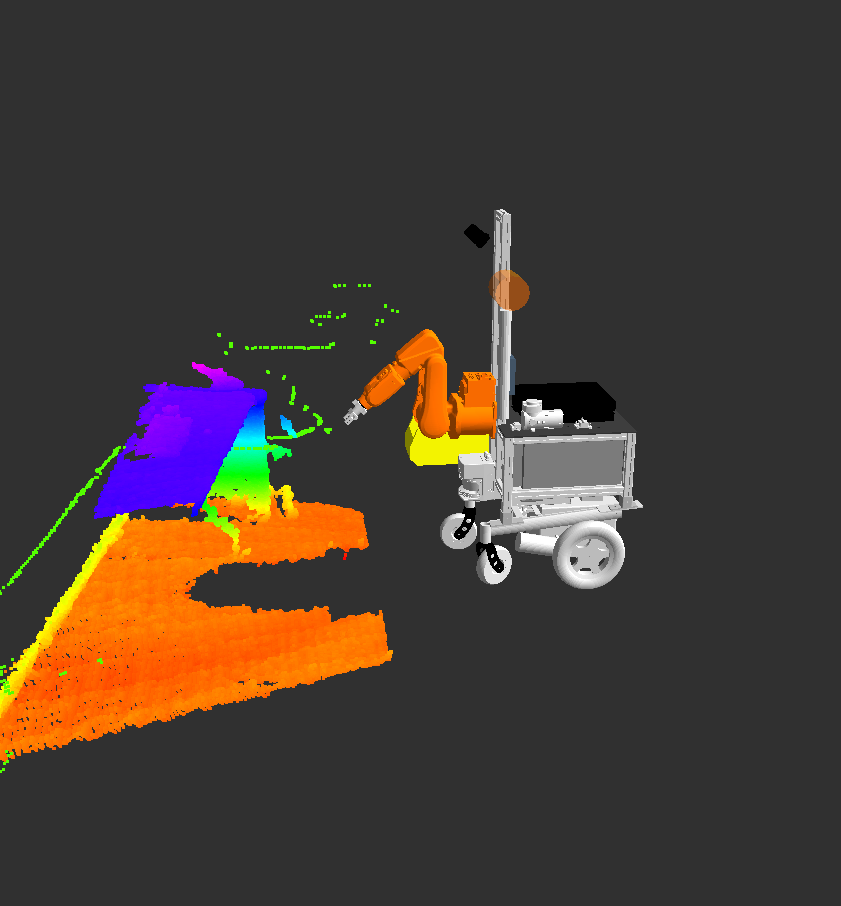
\includegraphics[width=6.0in]{rviz}
\caption{ABBY’s robot model, LIDAR data (green points), and Kinect point 
cloud (multicolored points) visualized in Rviz}
\label{fig:rviz}
\end{figure}

In addition to providing the geometric definition of the robot, the
robot model makes the Rviz robot visualization GUI much more usable.
Because visualization meshes of the robot are defined, Rviz can render
an accurate visualization of the robot in its current state. This is
useful for verifying that the state of the robot in ROS matches the
physical state of the robot. In an industrial environment, it would also
allow a user to remotely monitor a robot without the need for a CCTV
system external to the robot.

\section{Hardware Drivers}
\label{hardware-drivers}

ROS uses a
software driver implemented as a ROS node to read data from a sensor or
send commands to an actuator. The driver node for a sensor interfaces
with the sensor hardware and publishes data as ROS messages to the
appropriate ROS topic(s). The driver node for an actuator subscribes to
actuator commands on the appropriate ROS topic and interfaces with the
actuator hardware to execute the commands. ABBY's Kinect camera and SICK
LIDAR use preexisting open source drivers \cite{kinect} \cite{laser_drivers},
and the ROS driver node for the mobile base was developed previously by this 
lab for other robots using the same hardware, and required limited modification
for this robot \cite{harlie}. The driver for the ABB robotic arm was written
for this platform in collaboration with the Southwest Research Institute
(SWRI) of San Antonio, Texas as part of the ROS Industrial Project.

The mobile
base is controlled by software running on the cRIO, as described in Section
\ref{computing-hw}. The cRIO sends data to the PC containing information
about the robot's pose, the state of the power supplies, and raw count
data from the encoders. The PC sends angular and translational velocity
commands to the cRIO and may send commands to the cRIO to activate or
deactivate the emergency stop or to reboot the cRIO. These two tasks
(sending and receiving data) are handled by two different ROS nodes. A
third ROS node publishes pose information as a standard ROS message.

The receiving ROS node handles UDP packets from the cRIO. Encoder data
are checked to ensure that all of the encoders are updating properly,
and voltage data are checked to monitor the battery level and health of
the power regulator. The results of these checks are fed into a ROS
diagnostic updater, which provides feedback to the operator. Voltage
information is also published to a custom ROS message so that other
nodes on the robot can subscribe to the voltage data. Pose information
is published as a custom ROS message type and sent to the odometry
translator node. The odometry translator publishes the robot's pose
using ROS-standard odometry messages, which are used in ROS's planning
and localization packages.

The sending ROS node subscribes to ROS "twist" topics containing desired
rotational and translational velocity from the mobile base trajectory
planner and sends the commands to the cRIO as UDP packets. It also
provides a ROS service to reboot the cRIO and ROS services to enable and
disable the drive base motors with the emergency stop.

The gripper driver is a ROS node that runs natively on an Arduino's
AtMega 328 microcontroller using the ROS Serial framework. It sends and
receives ROS messages over the USB serial connection. A ROS node,
included in the ROS Serial package, runs on the PC and acts as a
transparent bridge between the ROS system and the ROS node on the
microcontroller. The ROS node on the microcontroller publishes joint
state messages describing the current position of the gripper plates and
provides a ROS service to open and close the gripper. The Fuerte version
of ROS Serial did not properly support ROS services \cite{venator_rosserial_ros_answers}. In order to
implement a service on the Arduino, changes were made to the ROS Serial
bridge node and microcontroller code to enable support of
services \cite{venator_rosserial_github}.

ABBY uses the ROS Industrial framework of messages and driver nodes to
control the IRB-120 using the IRC5 Compact. ROS Industrial is a project
led by SWRI to develop a standard ROS framework for using ROS with
industrial robots \cite{edwards}. ABBY's ROS Industrial driver was written
specifically for this project, and has been incorporated into the ROS
Industrial codebase.

Part of the ROS Industrial arm driver runs on the IRC5 Compact. The
software on the IRC5 Compact is written in RAPID, ABB's proprietary
programming language. The software running on the IRC5 Compact consists
of a trajectory server, a state server, and a motion process. The state
server periodically polls the positions of the joints in the arm and
sends that information to the ROS system. The trajectory server receives
trajectory packets from the ROS system and queues them for the motion
process. When the trajectory server receives a complete trajectory, it
passes the trajectory to the motion process, which sends the arm to each
point in the trajectory. In order to generate smooth motion through the
trajectory, the intermediate points in the trajectory are defined as
low-precision waypoints. Because RAPID only has fixed-length data
structures, trajectories must have a fixed maximum length. Paths
generated for the IRB-120 with the current planner software have been
experimentally determined not to exceed 300 points in most cases, so the
maximum trajectory length was set to 500.

The robotic arm driver, like the mobile base driver, consists of two ROS
nodes that communicate with a server running on the IRC5 robot
controller. ROS trajectory messages describe the trajectory of a robotic
arm as a series of points, with each point describing the position and
velocity of all of the robot's joints. One of the ROS nodes subscribes
to ROS trajectory messages, breaks them up into packets, and sends them
to the IRC5 controller over TCP using a standard packet structure
defined by SWRI. The other ROS node connects to the IRC5 controller over
TCP and listens for state information from the controller, which is sent
using another packet structure defined by SWRI. It publishes this state
information, consisting of all of the robot's joint angles, as ROS joint
state messages and ROS joint trajectory feedback messages. These
messages are used by other ROS nodes to determine the position of the
robot's arm and as feedback to the arm planning nodes \cite{venator_case}.

\chapter{Experimental Software}

New software packages were developed
and integrated with existing open source packages for ABBY. Some of
these packages increase the capabilities of the platform, and others
were used to test those capabilities. These include navigation and
planning, calibration procedures, and investigations into industrial
applications.

\section{Mobile Base Planning}


ABBY's mobile base is controlled by software that performs localization,
which determines where the robot is in its environment, high level path
planning, which determines a feasible course from the current location
to the desired location, and trajectory planning, which determines a
sequence of velocities for the robot to execute in order to arrive at
the desired location.

ABBY performs localization by fusing odometry and Adaptive Monte Carlo
localization methods to create a reliable, accurate estimate of the
robot's position. Two standard ROS mobile base planners develop global
and local plans to specified
waypoints.

\subsection{Localization}
\label{localization}

In robotics, localization is the task of determining where the robot is.
Localization methods can be classified into one of two groups. Relative
localization methods determine the robot's location with respect to the
robot's previous location, and absolute localization methods determine
the robot's location with respect to an absolute reference in the
robot's environment, sometimes called the ``ground truth.'' There are
advantages and disadvantages to both classes of localization methods,
and ABBY's localization uses a combination of relative and absolute
localization to mitigate the disadvantages and leverage the advantages
of each.

A benefit of relative localization methods is that they are
computationally simple. Odometry on ABBY uses fourteen mathematical
operations (seven addition, four multiplication, and three
trigonometric, as shown in Algorithm \ref{alg:odometry}.). This allows for high
frequency update rates and implementation on embedded processors or in
logic circuitry.

\begin{algorithm}
\caption{Odometry update from differential wheel encoder measurements. 
$d_r$ and $d_l$ are the difference in encoder counts since the last update. trans 
is the translation. $d_x$ and $d_y$ are the translation in the x and y directions. 
$d_{\theta}$ is the rotation in $\theta$, and $\theta$ is the heading.}
\label{alg:odometry}
\begin{algorithmic}
\STATE $d_r \gets r - r_0$
\STATE $d_l \gets l - l_0$
\STATE $trans \gets k_t * (d_i + d_r)$
\STATE $d_x \gets trans * cos(\theta)$
\STATE $d_y \gets trans * sin(\theta)$
\STATE $x \gets x_0 + d_x$
\STATE $y \gets y_0 + d_y$
\STATE $d_\theta \gets arcsin(k_\theta * (d_r - d_l))$
\STATE $\theta \gets \theta_0 + d_\theta$
\end{algorithmic}
\end{algorithm}

Further, relative localization requires no knowledge of the robot's
environment (such as a map), and it does not require the robot's
environment to be instrumented with sensors to track the robot or
beacons for the robot to track. Relative localization can also be
accomplished with relatively cheap sensors such as inertial measurement
units (IMUs), optical flow sensors, and (in the case of wheeled
vehicles) shaft encoders.

However, relative localization methods all accumulate error over time.
Each update is performed with respect to the previous, and the
superposition of successive errors causes the cumulative error to
increase. The source of the error may be physical, such as wheel slip,
or computational, such as the non-linearity of the trigonometric
function used to estimate the heading in Algorithm \ref{alg:odometry}. A 
well-calibrated relative localization system with an accurate observer model 
will still accumulate error over time, and the estimated position of the 
robot will slowly diverge from the true position. This was demonstrated using
ABBY's odometry system; see Section \ref{localization}.

Unlike relative localization, absolute localization does not accumulate
error. There are several different types of absolute localization
methods that use different types of sensors. Some methods use external
sensors, such as cameras or radio frequency (RF) tracking systems to
monitor the robot's position. In order for a robot to use these methods,
the operating environment must have already been instrumented with the
necessary sensors. Other methods use sensors on the robot to track
features of the robot's environment and compare them to a known map of
the robot's environment \cite{thrun}. Trackable features may already exist in
the environment, such as ceiling lights in an office building, or may be
added, such as position-coded labels on a warehouse floor. Systems with
ranging sensors can track features of the geometry of the environment
itself. To perform an update, all of these localization methods compare
sensor data to a map or model of the environment to estimate the robot's
position. This means that they are dependent on an accurate map or
model, which may not be possible in an environment with changing
features. Methods using sensors onboard the robot also depend on the
environment having suitable features to localize against, which may not
be true in environments such as open fields or environments with many
repeated similar or identical features such as long hallways.

Although most absolute localization methods require an \emph{a priori}
map (or model) of the environment, one class of absolute localization
methods performs simultaneous localization and mapping (SLAM). SLAM
algorithms begin with no map of the robot's environment and
incrementally build one as they explore. A SLAM algorithm using a LIDAR
can exploit partially-overlapping LIDAR scans to register new scans with
respect to previous scans. The translation and rotation required to
register the scan can be used to determine the robot's position with
respect to the previous position. Each new scan increases the known
region of the environment, slowly building a map \cite{thrun}.

ABBY's sensor suite contains several sensors that can be used for
localization. The encoders on the wheels are well-suited for odometry.
The LIDAR and the Kinect depth camera can both be used for absolute
localization using a number of methods, including both SLAM and \emph{a
priori} map localization algorithms. In addition, the Kinect camera
could be used for localization based on patterns on the floor. Of these
possible methods, odometry was chosen for relative localization, and
Adaptive Monte Carlo Localization (AMCL) using LIDAR scans and an
\emph{a priori} 2D occupancy grid map was chosen for absolute
localization.

ABBY uses odometry from the encoders on the wheels for relative
localization. The physical state observer runs under the real time
operating system on the cRIO, and publishes pose estimates with
uncertainty (represented as covariance) to the ROS system at 50 Hz.
Relatively high frequency updates to the robot's pose are required as an
input to the local planner, which generates velocity pairs at a rate of
12 Hz.

A SLAM algorithm was considered for absolute localization on ABBY.
Because SLAM does not require an \emph{a priori} map, it would be easy
to install a SLAMing robot in a novel environment. Maps were generated
by ABBY using the LIDAR and the gmapping SLAM package \cite{grisetti}. Gmapping
uses a Rao-Blackwellized particle filter to generate maps as it
localizes. Gmapping on ABBY was unable to reliably traverse doorways
without introducing error. This was sufficient reason not to use it for
localization.

Instead, the maps were manually cleaned up using image editing software
and used as \emph{a priori} maps for AMCL. AMCL is an absolute
localization method that models the robot's pose as a probability
distribution \cite{thrun}. The robot's pose is considered probabilistic to
represent the uncertainty of the sensor measurements used to determine
the pose. ABBY uses AMCL to match LIDAR scans to an \emph{a priori} map.
AMCL can theoretically solve the ``wake-up robot problem,'' in which the
robot is initialized with no estimated pose. However, testing with ABBY
showed that AMCL could not reliably solve this problem, and would often
converge on a false pose estimate. Instead, ABBY is initialized to a
pose at or near the true pose, with sufficiently large covariance that
the true pose is within the likely region of the estimated pose. As the
robot runs, the pose estimate will converge on the true pose. On ABBY,
each pose update from AMCL takes approximately 200 milliseconds, so it
can run no faster than 5 Hz.

Combining odometry with AMCL yields results that are better than either
one alone. Because AMCL takes so long to compute, it cannot be used to
approximate continuous localization. The local planner for the mobile
base updates at 12 Hz, which is faster than AMCL can update. Whereas
odometry is more suitable for the local planner, the error it
accumulates as the robot runs eventually makes it unsuitable for global
planning.

\begin{figure}[ht]
\centering
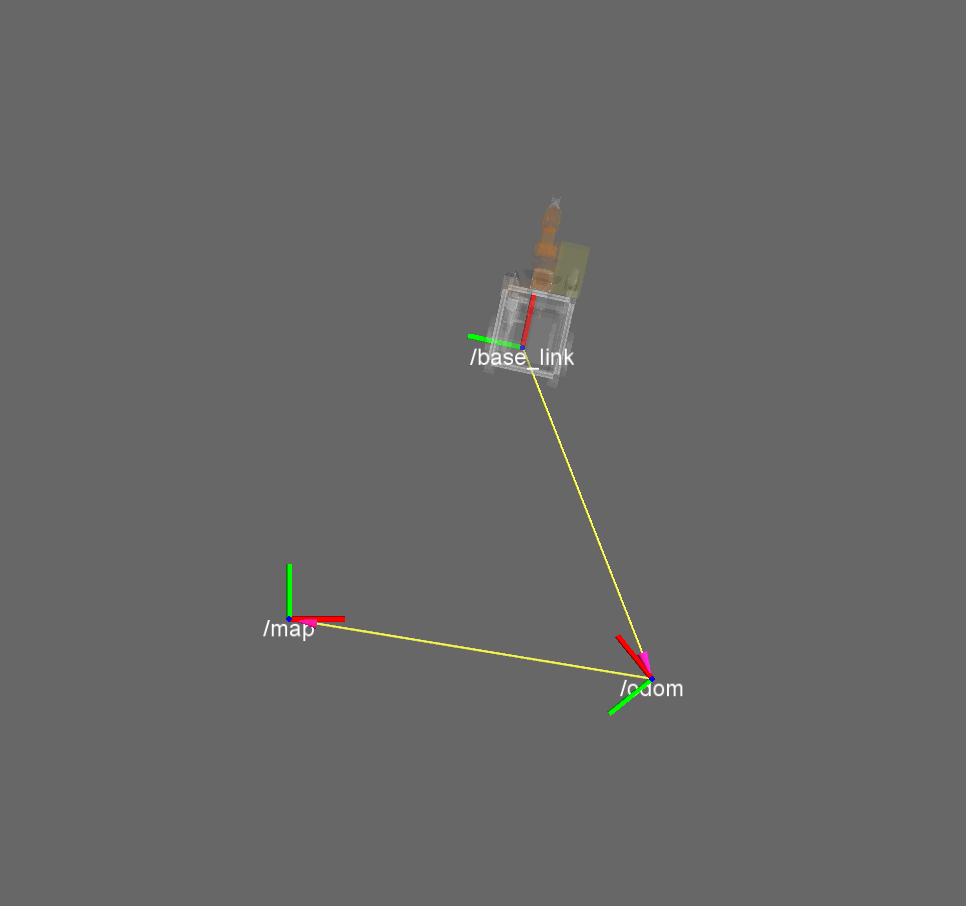
\includegraphics[height=4.0in]{odom_frames}
\caption{The map, odometry, and base frames of the robot localization system.}
\caption*{The transform from the world frame map to the odometry frame, 
generated by AMCL, cancels out the accumulated error in the transform from 
the odometry frame to the robot's base frame, generated by odometry.}
\label{fig:tfs}
\end{figure}

The results of two methods are fused by storing two transforms in the
robot's TF tree, as shown in Figure \ref{fig:tfs}. One transform is between the
robot's base\_link (a coordinate frame with its origin on the floor
between the robot's wheels) to its parent, the odometric frame odom.
This transform is updated by the odometric state estimator on the cRIO
at 50 Hz and provides a higher resolution position estimate. Local
planning is performed in the odom frame. The top level transform is from
the map frame (the absolute coordinate system) to the odom frame. This
transform is updated by AMCL, which runs an update every time the robot
moves more than 0.05 meters in translation or 0.1 radians in rotation.
On each AMCL update, the transform from the map to odom frame changes
such that it cancels out any error in the transform from the odom frame
to the robot's base\_link. Over a long period of operation, the odom
transform may accumulate significant error, but the transform from the
map frame to the base\_link remains accurate because of the absolute
localization updates.

\subsection{Mobile Base Trajectory Planning}

One of the major tasks for a mobile robot is navigation through its
environment. In an industrial application, the location may be retrieved
from an inventory database, or it may be specified by a human operator,
but the robot's task is the same. From its current location, the robot
must plan a path to another location in its environment. The path must
avoid obstacles, and it should be as direct and efficient as possible.
The robot must then generate a trajectory to follow the path and travel
to the goal location. The trajectory cannot violate the dynamic
constraints of the robot. Given a trajectory, the robot must execute it
by controlling the actuators as accurately as possible to adhere to the
desired path and trajectory.

Speed control on ABBY was implemented by previous researchers as a pair
of PID controllers, one for each wheel. The PID controllers are
implemented on the cRIO's FPGA for speed and robustness, with loop
closure rates of 100 Hz. A simple geometric algorithm (see Equations 1
and 2), implemented on the cRIO's PowerPC processor, is used to convert
twist-style commands (forward and rotational speed) into speed setpoints
for each wheel. Each PID controller's setpoint is specified in
meters/second and its output is an 8-bit signed integer These signed
integers represent the desired voltage to be output by the Sabertooth
motor controller, with -127 being full reverse and 127 being full
forward. Since the Sabertooth motor controller can vary its voltage
output from -24 volts to 24 volts, the 7 bits of speed resolution in
each direction correspond to a voltage output resolution of about 189mV.
The PID controllers on ABBY were originally tuned for another robot with
the same mobility platform but a different weight distribution \cite{yanick}.
With some retuning, ABBY's minimum achievable forward/reverse speed is
0.1 m/s and minimum rotational speed is 0.35 rad/sec; other robots based
on the same mobility platform were able to achieve 0.1 m/second and 0.1
radians/second respectively.

\begin{equation}
\label{eq1}
 v_{left} = v_x - \frac{w_{track}}{2} * v_{yaw}
\end{equation}

\begin{equation}
\label{eq2}
v_{right} = v_x + \frac{w_{track}}{2} * v_{yaw}
\end{equation}

The higher-level components of navigation are path and trajectory
planning. Path planning is the task of determining a path from the
robot's current location to a desired pose. Trajectory planning takes
the path and determines a series of velocity commands to move the robot
through the path without violating the acceleration and velocity
constraints of the robot. On ABBY, these tasks are performed by a global
and a local planner, respectively.

NavFn \cite{navfn}, the global planner node available in the ROS navigation
stack, operates on a grid-based global costmap populated by data from
the LIDAR. Given a desired pose, NavFn finds a minimum-cost path using
Dijkstra's algorithm \cite{dijkstra}. This path is defined as a series of
intermediate robot poses along the path. NavFn successfully plans paths
for ABBY in relatively open environments, but because it assumes a
circular robot base, it will sometimes plan impossible paths in crowded
environments.

The local planner generates trajectories to follow the path produced by
the global planner; it operates on a local costmap populated by data
from the LIDAR. The robot performs local planning using a trajectory
rollout approach \cite{thrun}, which forward-simulates translational and
rotational velocities and evaluates the resulting trajectories for
proximity to obstacles, proximity to the goal, and adherence to the
global path. These scores are weighted and summed to determine the
velocity command's score. The highest scoring velocity command is sent
to the mobile base driver

\section{Inverse Kinematics Solver}

An important part of robotic arm planning is an inverse kinematics
solver. Given a pose in the robotic arm's work envelope, an inverse
kinematics solver determines a set of joint angles that would place the
end effector at that pose. Because not all poses have possible solutions
and some poses are degenerate cases, analytical inverse kinematics
solvers are mathematically complex.

ROS includes a kinematic solver in the kinematics\_constraint\_aware
package that wraps the inverse kinematics solver of the Orocos project's
Kinematics and Dynamics Library (KDL) \cite{orocos} \cite{openrave}. The KDL solver is
a numerical solver that uses Newton-Raphson iterations. The KDL solver
takes joint angle limits into account in evaluation of its solutions,
only returning a solution with valid joint angles. However, the KDL
solver will often fail for achievable poses and, because it uses an
iterative numerical method, runs slowly, on the order of tens of
milliseconds.

To counteract the problem of the KDL solver failing for achievable
positions, the solver was wrapped in a method to retry the search on
failure. When the solver fails to find an inverse kinematics solution
for a desired pose, the solver is reseeded with randomly selected joint
values and called again, up to 100 times. To test the solver, poses were
generated using forward kinematics of simulated joint angles. Since the
poses were generated by forward kinematics, they are guaranteed to be
achievable. Many of the test poses were not solvable by the unmodified
kinematic solver, which only made one attempt at a solution. When the
number of attempts was increased to 100, the success rate was 32\% for
solvable poses.

\begin{figure}[ht]
\centering
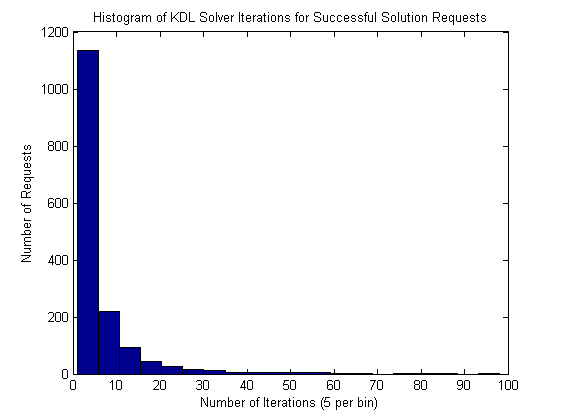
\includegraphics[width=6.0in]{KDL_histogram}
\caption{A histogram of the number of iterations required for the KDL inverse 
kinematics solver to solve for achievable pose requests.}
\caption*{5000 poses were requested, of which 1583 were solved in less than 
100 iterations.}
\label{fig:kdl-histo}
\end{figure}

As shown in Figure \ref{fig:kdl-histo}, most inverse kinematics requests are solved in
under 20 iterations or will fail. Since the seed is random, the number
of requests needed to solve for a difficult pose is probabilistic, and
though some positions are more difficult to solve for using KDL's
iterative approach, there is no guarantee that the solver will succeed
or fail for a given pose. The resulting inverse kinematics solver is
suitably reliable, though slow, taking as long as 3.5 seconds before
determining that a pose is unsolvable. This is acceptable for the robot
at this time, but a faster, more reliable inverse kinematics solver will
be necessary in an industrial installation.

The OpenRAVE project includes the IKFast kinematic solver tool \cite{openrave},
which analyzes a kinematic chain and generates C++ code for an inverse
kinematics solver for that chain. The solver it generates is a
closed-form analytic solver, meaning it runs very quickly (\textless{}1
ms) and can handle the vast majority of achievable poses, including
degenerate cases. The greatest limitation of IKFast is that it does not
take into account joint limits, but assumes that all joints can rotate
freely. This means that IKFast will often generate solutions that are
unachievable for a rotation-limited robotic arm.

The ROS wrapper for IKFast rejects solutions that violate joint
constraints, but IKFast will only return the first eight IK solutions it
finds, and it is likely that none of these solutions will satisfy joint
constraints, particularly for degenerate cases. When this happens, the
ROS inverse kinematics service fails, despite the possible existence of
a valid solution. It may be possible to rewrite the IKFast compiler or
modify the generated code to work with joint limits, but at this time,
IKFast was determined to be unsuitable for arms of ABBY's geometry due
to the high incidence of solver failure.

\section{Arm Navigation}
\label{arm-nav}

ABBY's arm navigation package is closely based on the standard ROS arm
navigation package, which is generated from a URDF by a tool called the
Planning Description Configuration Wizard. This wizard allows the user
to define a manipulator kinematic chain from a URDF file and then
generates an arm navigation application, including the necessary launch
files for an inverse kinematics plugin, a planner, and a collision
environment server. This "default" arm navigation application was
augmented with filtering nodes for the Kinect data going into the
collision environment and the modified KDL inverse kinematics plugin
described above.

The trajectory planner for the arm is the default planner available with
the ROS arm navigation package. It uses a sample-based planning
algorithm from the Open Motion Planning Library called Single-Query
Bi-Directional Probabilistic Roadmap Planner with Lazy Collision
Checking (SBL) \cite{sanchez}. SBL plans collision-free paths for the arm and
publishes these paths as ROS trajectory messages, which the ROS
Industrial arm driver executes. Because SBL performs all of its planning
in joint-space, the arm navigation application uses the inverse
kinematics plugin described above to convert goal poses into joint space
before planning paths to them.

\subsection{Collision Detection}

The robot uses the ROS node Collider to maintain a collision map, a 3D
occupancy grid represented by an Octomap oct-tree. The collision map is
populated by data from filtered Kinect point clouds. In addition to this
"raw" map, a collision environment is maintained, which contains
information from this map and keeps track of detected objects such as
the manipulable objects detected by the tabletop box recognition system
described below. The objects are given IDs and stored in the map as
meshes or geometric solids, enabling the arm navigation code to make
decisions about whether collisions are allowable.

The arm navigation code navigates around obstacles in the collision
environment, including the robot itself, preventing the robot from
damaging itself and the objects around it. Collisions can be selectively
allowed between robot links and objects in the collision environment.
For instance, it is impossible to pick up an object without the jaws of
the gripper colliding with it. When creating a request to make the final
approach to pick up an object, collision detection between the gripper
jaws and the object is disabled, allowing the robot to pick the object
up while still preventing collisions between the robot and other
obstacles.

\subsection{Kinect Data Filtering}

The Kinect's field of view includes the robot's arm, which the collision
detection process would classify as obstacles. This causes the robot to
freeze because it is in collision with a perceived obstacle, even though
the obstacle is the robot itself. In order to prevent this, the Kinect
point cloud is pre-filtered to remove points that are within the robot
volume, which is determined by padding the 3D model of the robot
generated from the URDF. The resulting point cloud, which has all points
within the robot removed, is used for all collision monitoring and
object detection. This is a computationally intensive task, consuming
one full core of the PC's processor.

\section{Tabletop Box Manipulation}
\label{tabletop-manip}

Once ABBY arrives at the desired location in the factory, it must
identify objects and pick them up from the inventory shelves. This is an
area of future research, but a basic object perception and manipulation
system was implemented as a proof of concept. The system uses several
object detection nodes developed by Willow Garage for the PR2 robot, as
well as two nodes written specifically for this project.

\begin{figure}[ht]
\centering
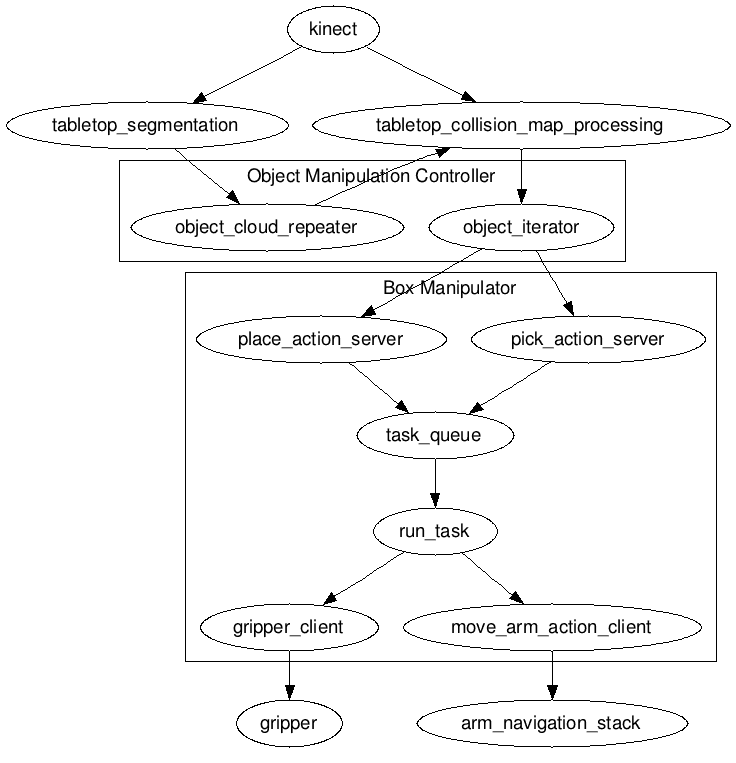
\includegraphics[width=6.0in]{box_manipulator_graph}
\caption{The box manipulation pipeline}
\caption*{Data from the Kinect is used to locate boxes on a table, which are 
then picked up and placed in the bin.}
\label{fig:box-manip}
\end{figure}

The Object Manipulation Controller was written specifically for this
project and serves as the central control node, translating and routing
messages between the perception and manipulation nodes. It provides a
callable method pick\_objects(), which performs the task described in
Algorithm \ref{alg2}.

\begin{algorithm}
\caption{The process for detecting, picking up, and stowing the objects
on a table.}
\label{alg2}
\begin{algorithmic}

\STATE $detected\_objects \gets$ tabletop\_detection($kinect\_data$)
\FORALL{$object$ in $detected\_objects$}
  \IF{graspable($object$)}
    \STATE pick($object$)
    \STATE place($object$)
    \STATE stow\_arm
  \ENDIF
\ENDFOR
\end{algorithmic}
\end{algorithm}

The tabletop\_detection() step is performed by the
tabletop\_object\_segmentation package, developed by Willow
Garage \cite{tabletop_object_detector} for the PR2 robot. This software identifies a tabletop
surface in a point cloud from the Kinect using RANSAC \cite{fischler} and adds
it to the collision environment as an object. Objects on top of the
table (detected\_objects) are segmented into separate point clouds and
inserted into the collision environment as Graspable Objects. These
Graspable Objects are used later by the manipulation package during the
pick() step to identify and locate the objects in the robot's
environment. The pick() and place() steps are performed by the box
manipulator node, which exposes them as action services using a standard
pick-and-place API defined in ROS. This standard API allows the box
manipulation package to be easily replaced by a new manipulation package
or the manipulation controller to be replaced by a more sophisticated
package. In the final step, stow\_arm(), the arm is moved to a
predefined stowed position, which minimizes the robot's footprint while
it is driving.

\subsection{Box Manipulation}

The box manipulator node was written for this project to lift small
objects from a shelf or table and place them. It provides two
services---one to pick up a graspable object, and one to place the
currently held graspable object at a set of coordinates.

When the manipulation controller calls the pick service on a Graspable
Object in detected\_objects, it uses another node created by Willow
Garage for the PR2 to fit a bounding box to the Graspable Object's point
cloud. Though the objects being manipulated are cylinders, a bounding
box is a fairly accurate representation of the object. This bounding box
is then used to generate an approach path composed of two poses. The
first is a pregrasp pose close to the object, with the gripper pointed
at the object center and the gripper jaws parallel to the sides of the
bounding box. This pose is sent to the arm navigation package, which
generates a trajectory and moves the arm to the pose. The second pose is
the grasp pose, with the object between the gripper jaws. This pose is
also sent to the arm navigation package, and once the robot is in the
grasp pose, the gripper is closed around the object.

Once the gripper is closed around the object, the object manipulation
controller calls the place service with a pose above the robot's onboard
storage bin as a target. This service sends the pose to the arm
navigation package, which generates a trajectory and moves the arm to
the bin. The gripper is then opened, dropping the object in the bin.

\section{Calibration}

In order for the point cloud data from the Kinect to be usable for arm
navigation, the positions of the Kinect and the arm must be correctly
registered in 3D space. Because the position of the Kinect camera's
optical frames within its housing are not precisely known, it was
necessary to perform a simple extrinsic calibration routine to determine
the position and yaw angle of this frame.

To determine the height (z-axis position) and pitch angle of the Kinect,
the robot was placed so the Kinect had an unobstructed view of the floor
in front of it. RANSAC \cite{fischler} was used to fit a plane to the floor, and
the transform from the fitted plane to the Kinect was calculated. A
similar method was used to determine the x-axis position of the Kinect.
The robot was placed so that the Kinect had an unobstructed view of a
wall at a known distance in front of it, and RANSAC was used to fit a
plane to the wall. The distance of the wall plane was then used to
calculate the x-axis position of the Kinect. The y-axis position of the
camera was estimated to be centered on the robot, and the y-positions of
the lenses were determined from the CAD model of the Kinect.

With the position of the Kinect now known, it was necessary to precisely
determine the pose of the arm relative to the Kinect. Due to the length
of the arm, a small error in the orientation of the arm could cause
significant disparity between coordinates in the Kinect's frame of
reference and the position of the robot's gripper calculated using
forward kinematics. The pose of the arm base was originally taken from
the CAD models used to design the robot, but the model's fidelity to the
robot was not sufficiently precise.

A more precise transform was calculated from test data using
Mathematica. Given a set of data points, the program calculates the
transform (translation and rotation) between the Kinect and the arm base
link that minimizes RMS error in the position of the gripper tip. Each
data point consists of the position of the tip of the gripper with
respect to the Kinect, measured from a manually-selected point in the
Kinect point cloud, and the pose (position and orientation) of the
gripper with respect to the base link of the arm, calculated by ROS's TF
server using forward kinematics. This program was run using an input
dataset of twenty-five points, and the resulting transform was used in
the robot's URDF to define the position of the arm with respect to the
Kinect.

\section{QR Code Recognition and 3D Localization}

Mobile manipulators in industrial settings can benefit from information
about the objects they manipulate. Most of the explorations of object
manipulation have been directed toward general purpose object
recognition and manipulation, but the problem of determining how to pick
up an object can be greatly simplified by simply putting manipulation
information on the object itself. For more complex information, the
object could link back to an entry in a database. Properties salient to
mobile industrial manipulation, such as grasp affordances, mass,
volumetric data, and visual cues for registration and localization, can
all be encoded into visual or RFID tags on manipulable objects. To this
end, an exploration was made into using the Kinect in conjunction with a
higher-resolution camera to read QR code tags on boxes and use the QR
code to perform 3D localization of the box.

QR codes can hold up to 3 kilobytes of data, or 174 bytes with 7\% error
correction. They include 3 "finder square" fiducials, which can be used
to acquire and correct the skew and size of the code. QR codes are
already used throughout the automotive industry for part
labeling \cite{qr}.

\begin{figure}[ht]
\centering

\includegraphics[width=2.3in]{Qr-3}
\caption{QR Level 3 code}
\caption*{(Source: Wikipedia, licensed under Creative Commons Attribution 
Share-Alike License)}
\label{fig:qr}

\end{figure}

Information about how to grip an object can be stored in a small amount
of data in a QR code on an object. This information, the ``affordance
cue,'' contains, in a compact form, information that aids a robot in
deciding how to manipulate an object:

\begin{enumerate}
\def\labelenumi{\arabic{enumi}.}
\item
  If an object has handles, the affordance cue contains the information
  necessary to define the handles and locate them relative to the tag.
\item
  If an object can be lifted only from the bottom, as with a fork-lift,
  the affordance cue contains information necessary to locate the bottom
  of the object relative to the tag.
\item
  If the object can be grabbed from the sides by a gripper, the
  affordance cue contains gripping force constraints and the information
  necessary to locate the sides relative to the tag.
\end{enumerate}

\begin{figure}[ht]
\centering

\includegraphics[height=2.5in]{Qr-3}
\caption{A box localized using the QR code.}
\caption*{Red dots are the QR code finder pattern. Blue is the projected 
handle center. Green are the handle corners.}
\label{fig:qr_box}
\end{figure}

Using a Kinect sensor and MatLab, a rudimentary proof-of-concept was
tested for boxes with handles on top. Because the Kinect image sensor
does not have high enough resolution to read QR codes, it must be
supplemented with a second, higher resolution camera extrinsically
calibrated to the Kinect. This part of the detection was simulated, and
the QR code data manually entered into the program. The coordinates of
the three finder points in the Kinect RGBD image are then used to get
the positions of the three finder points in 3D space. Again, because a
high resolution camera was not available, this step was simulated by
manually picking points. Using the 3D coordinates of the 3 finder
points, it is possible to localize the QR code in 3D space, including
both position and orientation. Using the location of the tag and the
tag's information about the handle's location relative to the tag, the
handle can be located, allowing a robot to grasp it without knowing any
other information about the box. The results are shown in Figure 
\ref{fig:qr_box}.

Because the Kinect RGB camera does not have sufficiently high resolution
for the task, these experiments were not performed on the robot.
However, this line of research is one of the planned future purposes of
the robot, once a high resolution camera can be acquired, mounted, and
calibrated to the Kinect.

\chapter{Industrial Safety}

Mobile robots, particularly experimental platforms, require safety
systems to disable them. These systems fall into two major categories.
Reflexive collision avoidance systems keep robots from colliding with
humans interacting with the robot. Emergency stop systems are used to
disable the robot in case it does something unsafe or unexpected. Both
types of systems are necessary in an industrial robot, especially one
that does not operate in a cage or with guards, neither of which are
practical for a mobile robot.

\section{Reflexive Collision Avoidance}
\label{reflexive-avoidance}

A key safety feature of many robots is reflexive speed limiting or
halting. Reflexive collision avoidance uses sensors to detect obstacles
in the robot's path and prevent motion that would result in a collision.
Reflexive collision avoidance is particularly important for robots that
operate in shared environments with people, because people can suddenly
move into a previously clear robot path, endangering themselves and the
robot. Whereas a planner will create safe paths for a robot around
static obstacles, paths may be invalidated by moving obstacles such as
people, and the planner may react too slowly to prevent a collision.
Reflexive collision avoidance operates more quickly and on a lower level
than planning and trajectory generation, and can override the velocity
commands from the trajectory generator.

At this time, ABBY does not implement reflexive collision avoidance for
the base or the manipulator. Because both operate at low speeds, the
robot does not pose a safety threat to the operator and can be easily
stopped with the emergency stop system described below. Before the robot
can be tested or deployed in an industrial environment, and to allow for
faster movement, reflexive collision avoidance must be added. Proposed
methods for reflexive collision avoidance are described in Appendix
3.

\section{Emergency Stop System}
\label{estop}

\subsection{E-Stop Systems Used in This Lab}

The Case Mobile Robotics Group has used a few emergency stop systems in
its robots. All of the HARLIE-class robots developed for the Intelligent
Ground Vehicle Competition used a commercially-available wireless relay
system from Remote Control Technologies. This system consisted of the
remote control relay in series with an onboard disable switch and a
second relay switched by an active-high enable signal from the cRIO,
which is software-controllable. These three switches (one manual and two
relay) control the current through the coil of a solenoid, which in turn
switches the power to the motor controller on and off. This system has
one critical flaw, which is that there is no ``heartbeat'' from the
wireless remote to the remote control relay. This means that if the
battery in the wireless remote dies or the radio communication is lost
between the wireless remote and the robot, there is no way to remotely
stop the robot, nor is there any indicator to the operator that the
robot cannot be wirelessly stopped.

OTTO the smart wheelchair could operate in either autonomous or manual
control modes, and used a custom remote system to enable and disable
autonomous mode. Using the GPIO mirroring function of a pair of XBee 2
Pro wireless network modules, a digital signal was transmitted from a
remote control unit to the input of the Arduino controlling the
wheelchair's motor controllers, disabling the autonomous functions of
the wheelchair when a button was pushed on the remote. Because the XBee
wireless modules' GPIO mirroring has a programmable timeout and default
output state, this system automatically disabled autonomous functions if
communication was lost between the remote and the robot. However, this
system relied on an Arduino microcontroller and was not designed as an
emergency stop system, but as a switch between autonomous operation and
normal (joystick) operation of a wheelchair.

\subsection{E-Stop Requirements}


This robot has several requirements that motivated the development of a
new emergency stop system combining the merits of the HARLIE-class stop
system and the OTTO remote switching system. First, the emergency stop
system needs to be able to switch the high current, 24 volt rail
providing power to the motor controllers. Second, the system needs to be
able to activate the 24 volt emergency stop input on the IRC5 robot
controller, which must be electrically isolated from the rest of the
robot's DC electronics. Third, the system must monitor four sources,
stopping the actuators if any of them are disabled:

\begin{itemize}
\item
  5 volt active-high enable signal from the cRIO, which is controlled by
  the ROS software
\item
  24 volt active-high emergency stop signal from the IRC5, which is
  controlled by the emergency stop switches on the IRC5 and FlexPendant
  and by RAPID software.
\item
  Twist-lock stop switch mounted on the robot (The robot is disabled if
  the switch is opened or disconnected.)
\item
  Wireless remote control with a heartbeat signal of at least 1Hz
\end{itemize}

Fourth, the system should be implemented entirely in hardware for safety
reasons. Software faults in a safety system are unacceptable and
adequate testing of a software system would be too time-consuming for
this project. Fifth, the remote control unit should have some feedback
as to the state of the four emergency stop sources described above.

Given the requirements, an emergency stop system was designed and
fabricated using printed circuit boards. The schematic of the system is
shown in Figure \ref{fig:estop-remote} and Figure \ref{fig:estop-receiver}. 
The system consists of two circuits, a remote control and an emergency stop 
circuit on the robot.

\begin{figure}[ht]
\centering
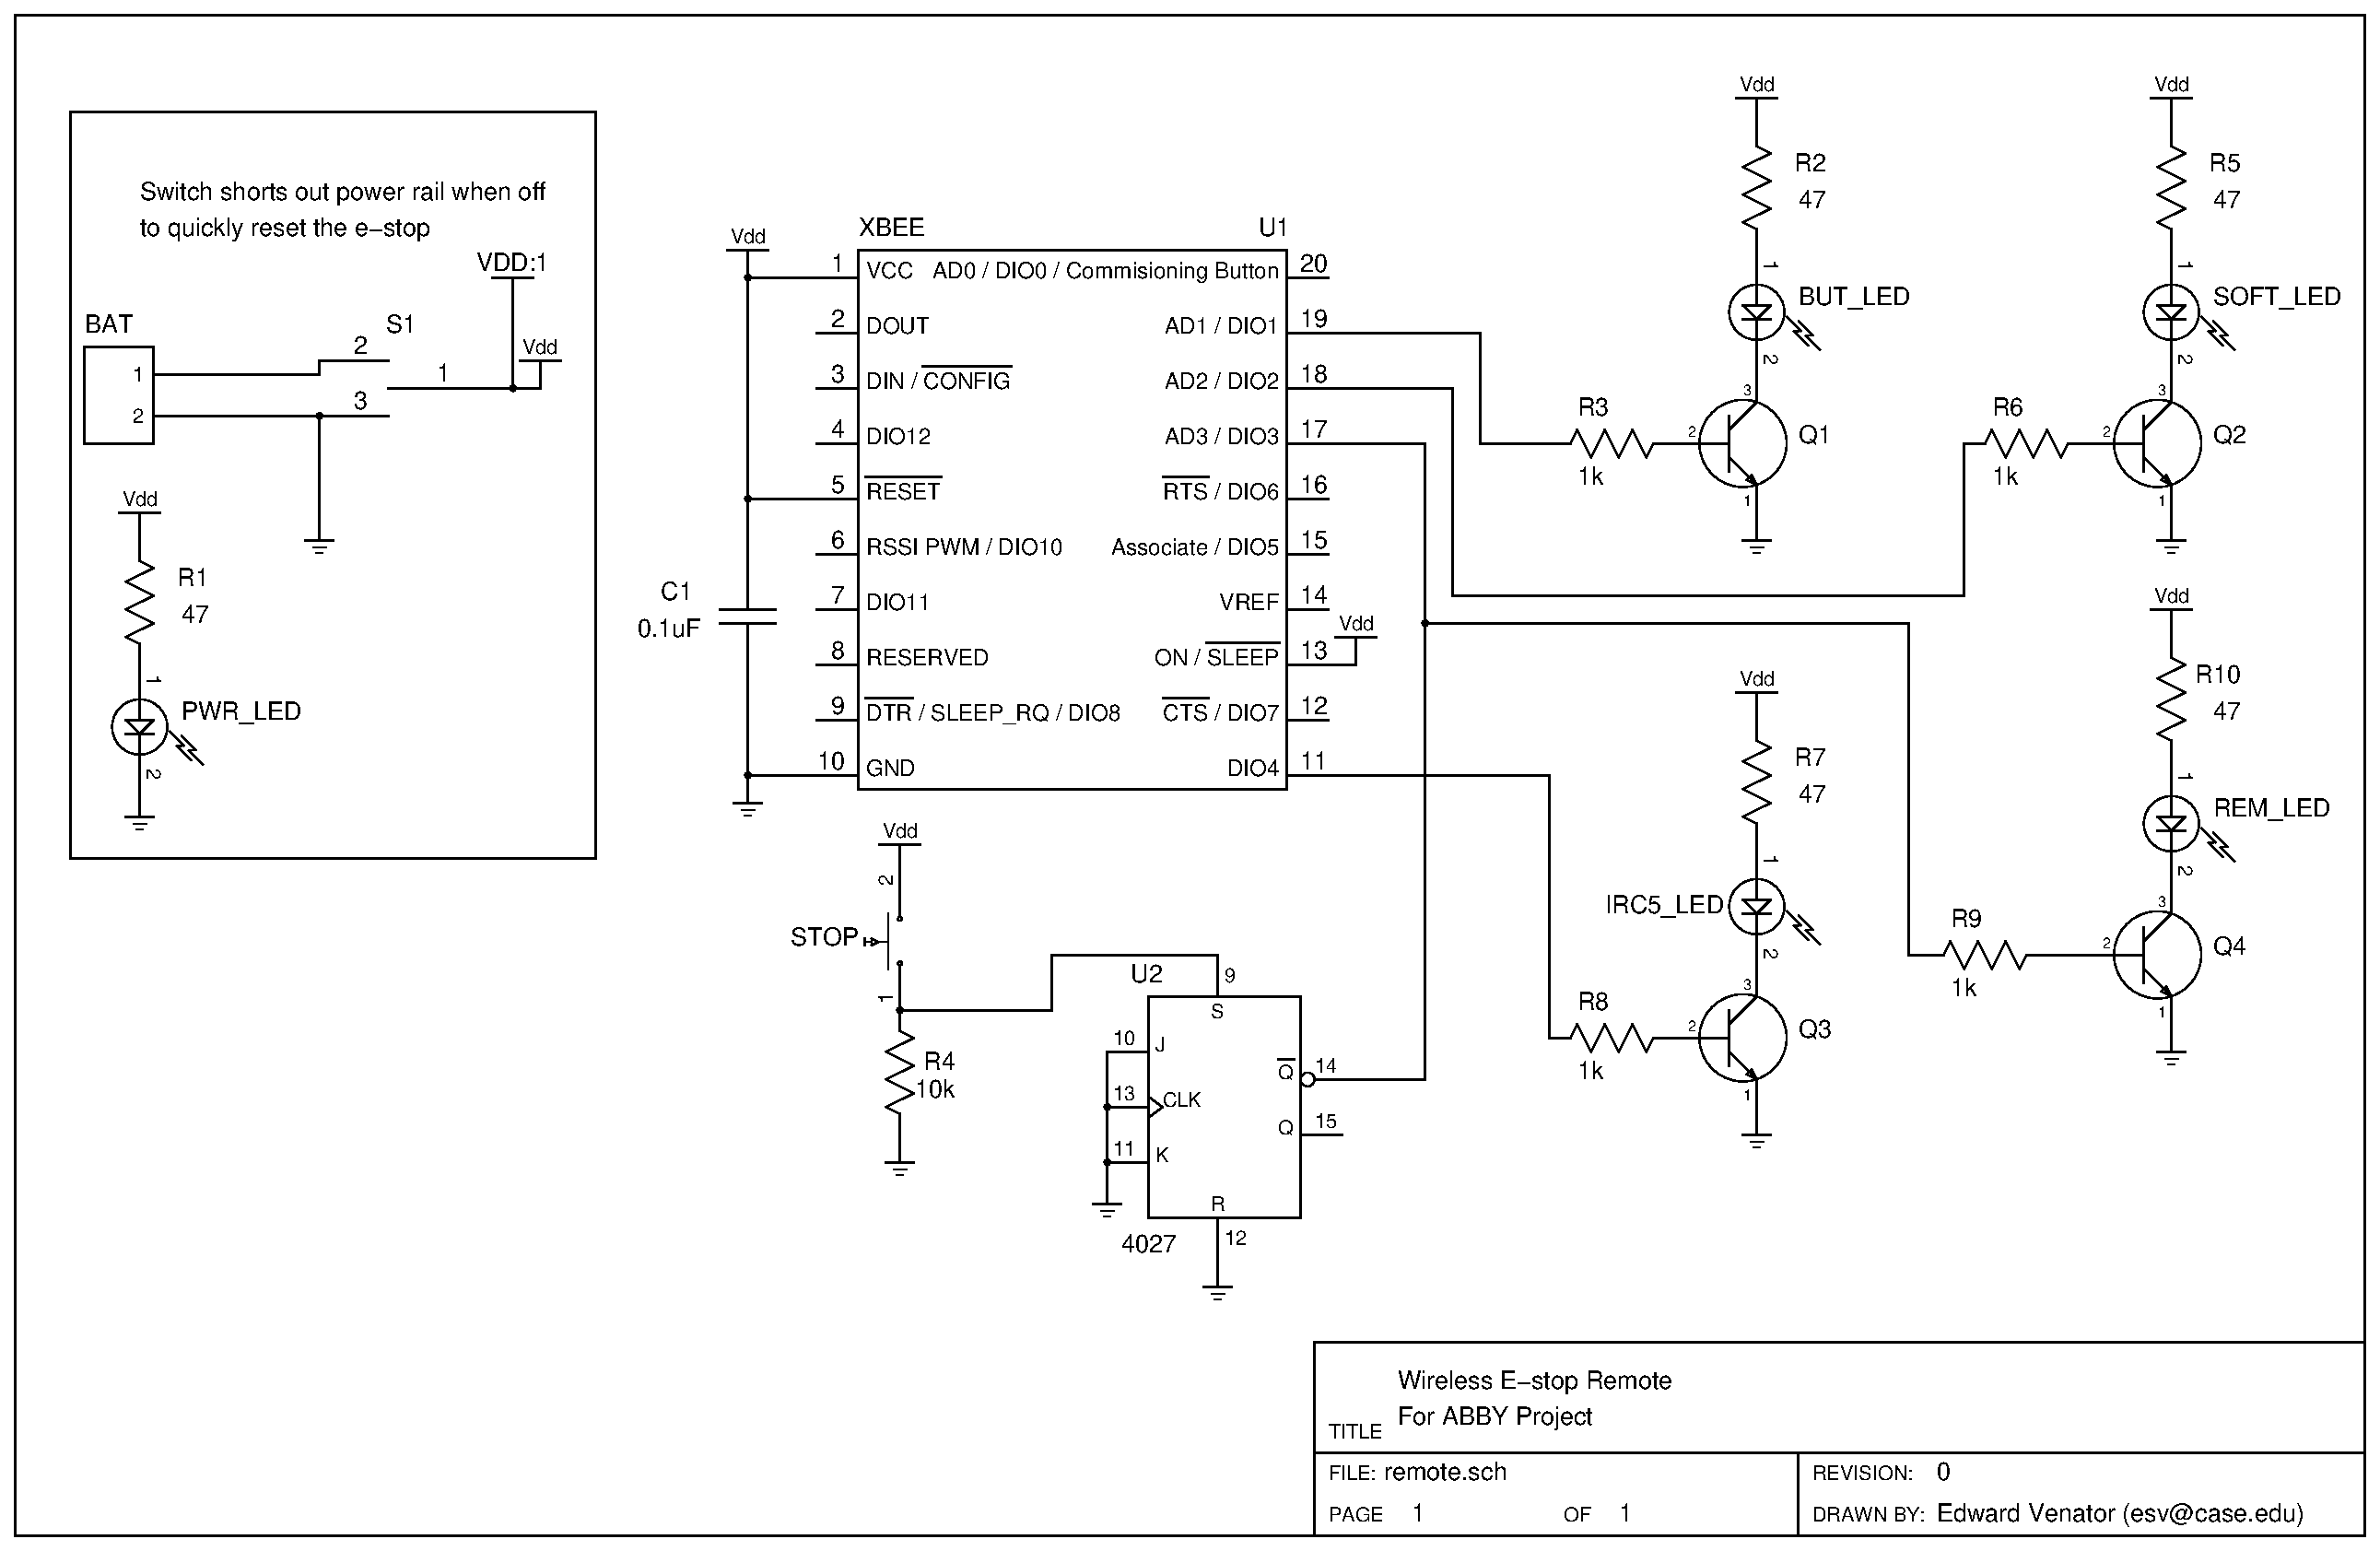
\includegraphics[width=6.0in]{estop_remote}
\caption{Schematic of the emergency stop remote tested on ABBY.}
\caption*{The remote uses an XBee radio to send an enable signal to 
the robot and receive the current emergency stop status from the robot, 
which is displayed with LEDs.}
\label{fig:estop-remote}
\end{figure}

\begin{figure}[ht]
\centering
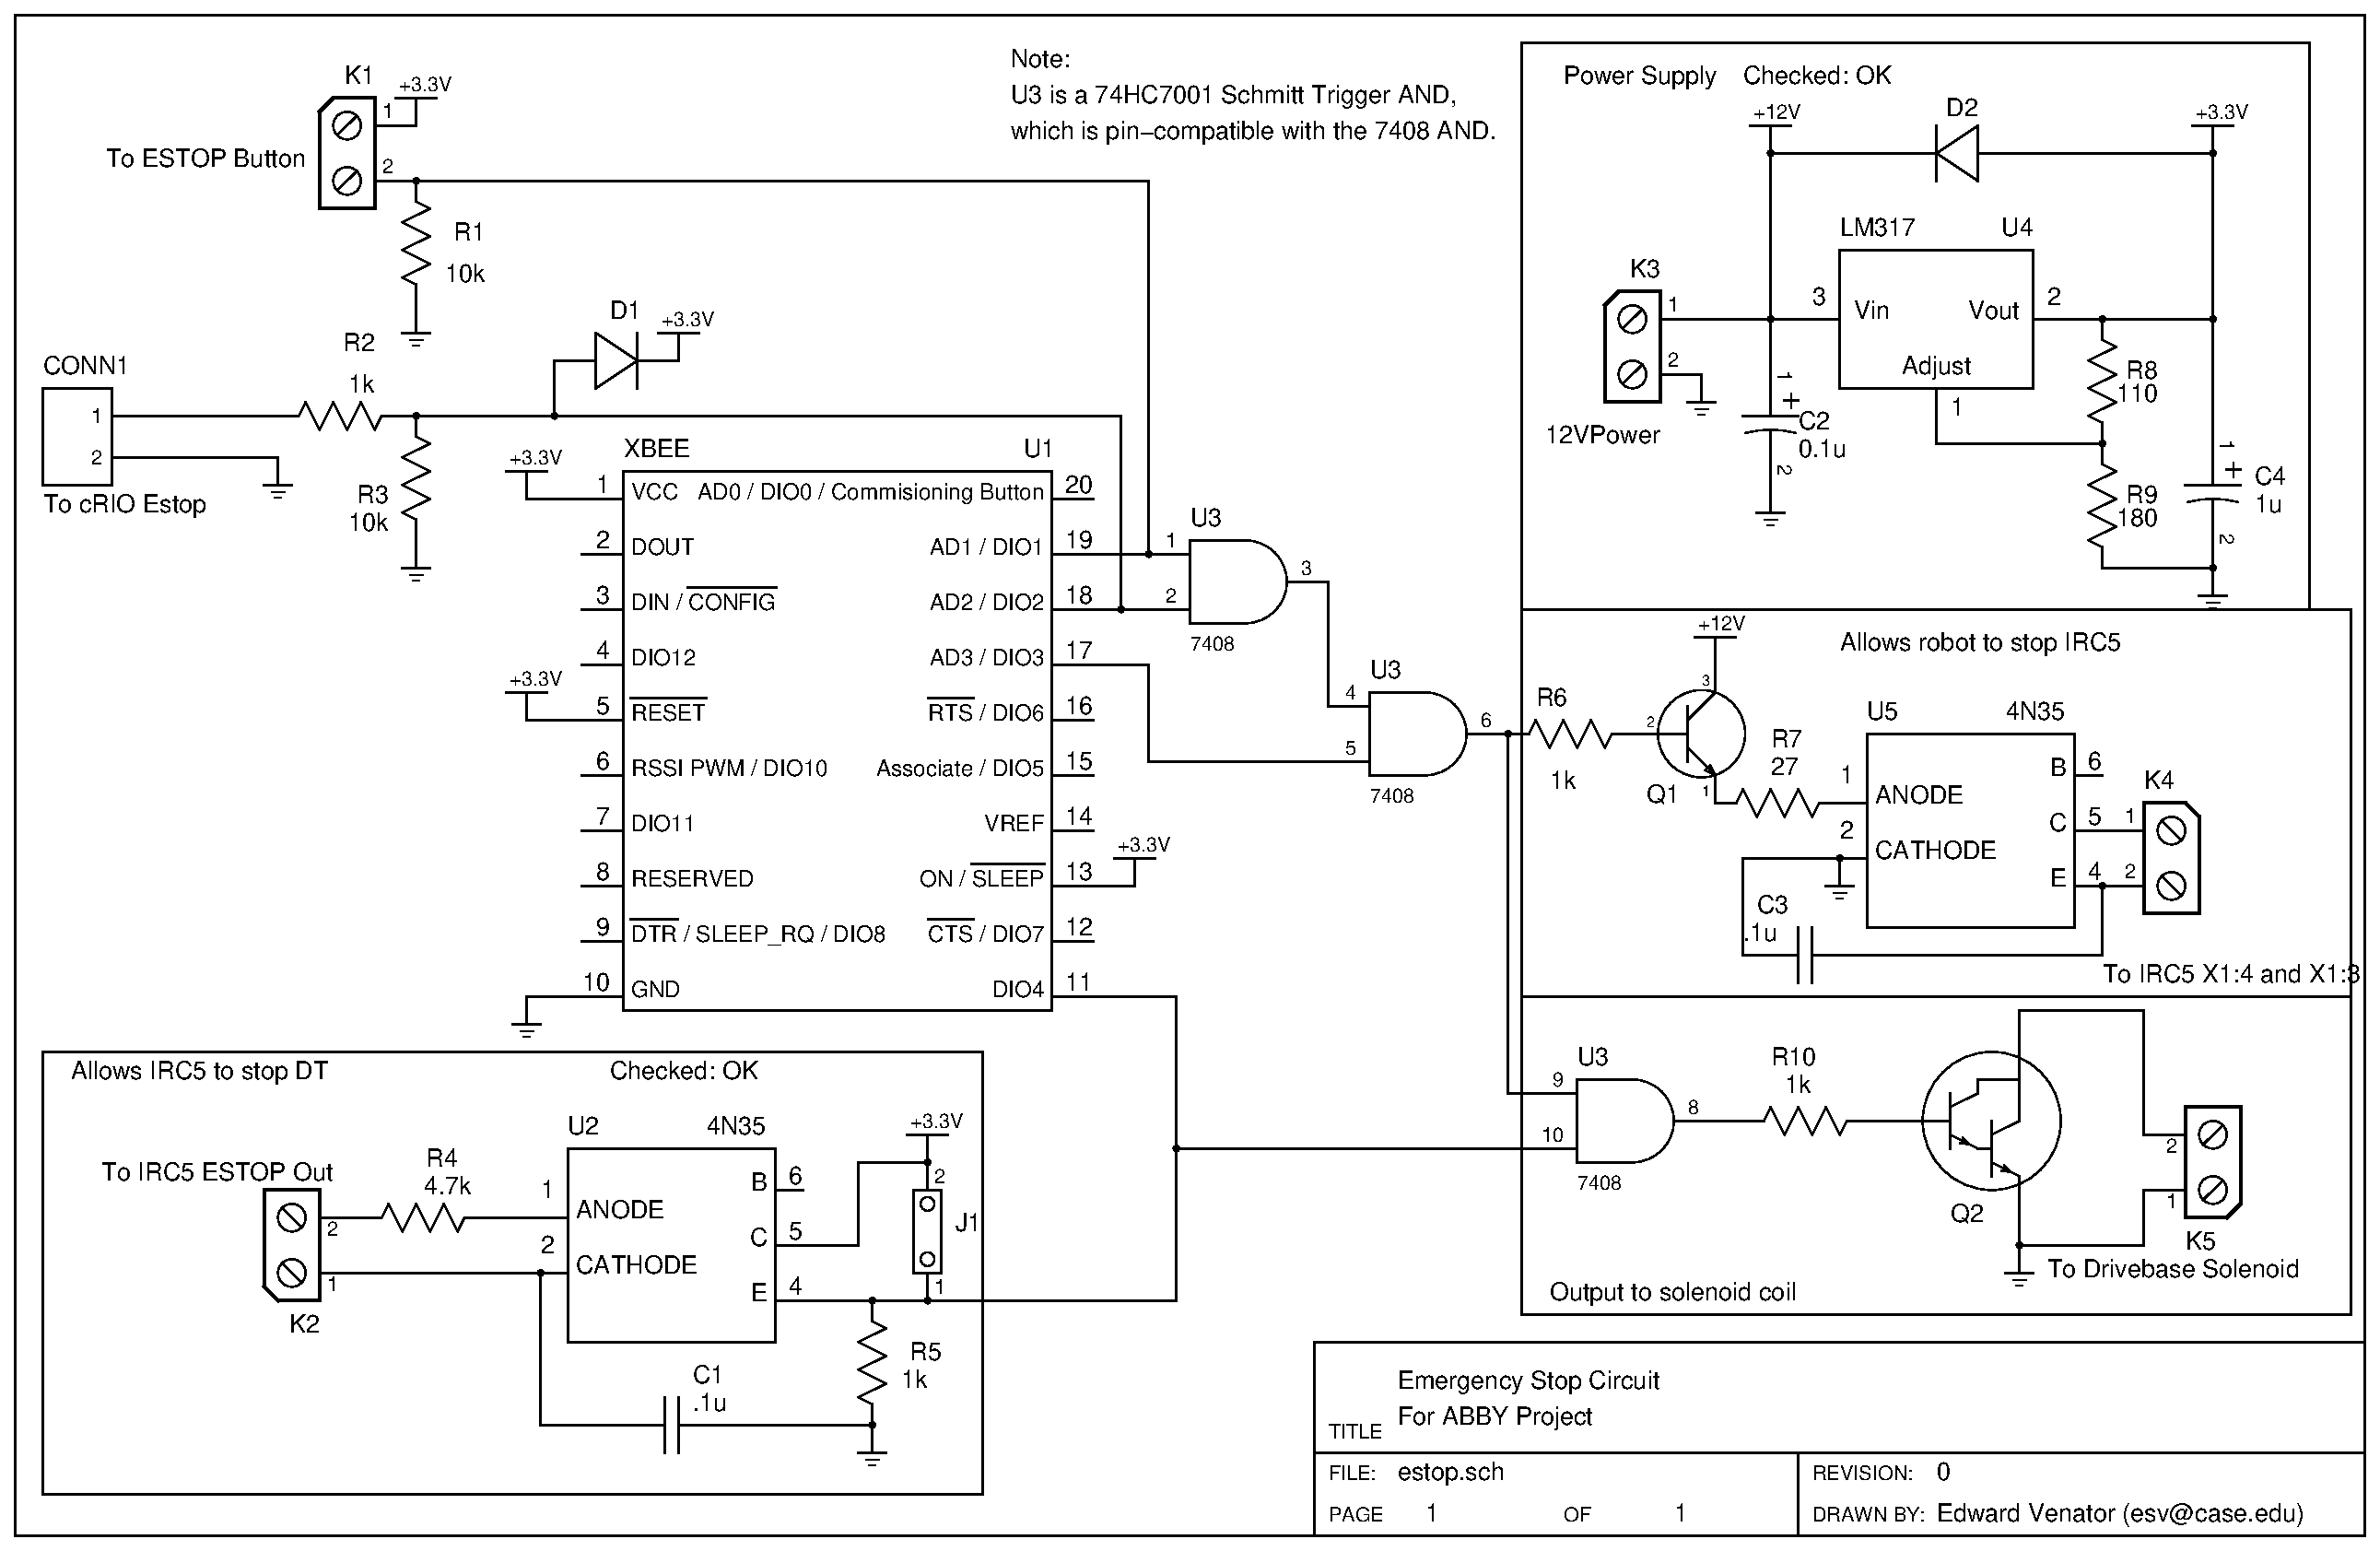
\includegraphics[width=6.0in]{estop_receiver}
\caption{Schematic of the emergency stop receiver and aggregator on ABBY}
\label{fig:estop-receiver}
\end{figure}

The remote circuit uses an XBee radio module's GPIO mirroring function
to transmit the state of the emergency stop button to the emergency stop
circuit on the robot in the same manner it was used on OTTO. This system
also uses the GPIO mirroring function to send the states of the onboard
emergency stop sources to the remote, where they are displayed on LEDs.
Because a twist-lock style emergency stop button was not available, an
S-R latch was used to latch the state of a normally-open momentary
pushbutton, requiring that the remote be powered off and back on again
to reset the wireless emergency stop. If communication between the XBEE
modems in interrupted for any reason, DIO3 in the emergency stop circuit
goes low, disabling the robot.

The emergency stop circuit on the robot has inputs for the onboard
emergency stop button, the cRIO's enable signal, and the emergency stop
output of the IRC5. The input from the IRC5 goes into an optoisolator IC
because the I/O on the IRC5 is floating relative to the rest of the
robot's DC systems. A 7400 series AND IC is used to generate logic
signals to enable the drive base and the IRC5's emergency stop input.
The drive base logic signal controls a Darlington transistor, which in
turn switches the coil of a solenoid that controls the drive base in the
same manner as on HARLIE-class robots (not shown in Figure 
\ref{fig:estop-receiver}; see Figure \ref{fig:power-schematic}). The IRC5 
output logic signal switches the 24v General Stop input of the IRC5 using 
an optoisolator IC.

These circuits were prototyped and installed on the robot. Because the
RAPID software running on the IRC5 was not configured to output the
emergency stop state, the input from the IRC5's emergency stop was
defeated by installing jumper J1. Additionally, testing showed that the
4N35 optoisolator used to switch the IRC5's emergency stop could not
sink enough current to enable the emergency stop circuit, causing the
IRC5 to go into General Stop mode seemingly at random. The ability to
control the IRC5's emergency stop state was defeated by disconnecting
the IRC5 Stop output and shorting the General Stop input on the IRC5.
These two changes completely decouple this emergency stop circuit from
the IRC5. Furthermore, the wireless link between the XBee modules proved
unreliable, causing the system to momentarily switch into emergency stop
mode seemingly at random. Extensive bench testing of the system suggests
that this problem is caused by an insufficiently reliable power supply
to one or both of the XBee modules. In order to make the system usable,
the wireless emergency stop was replaced with a twist-lock style
emergency stop button on a ten foot wired tether. The system does
reliably control the power to the drive base, providing a level of
safety for the robot, but revisions are required to gain the full
functionality of the original design.

A revised version of this emergency stop system is described in Appendix
2. The revised version has been designed, and all of its subsystems have
been tested, but it has not yet been implemented on the robot. The
revised emergency stop system includes a wireless remote and full
integration with the IRC5's emergency stop systems.

\chapter{Validation Results}

\section{Localization}

ABBY's odometry system was evaluated by performing two tests without the
benefit of an absolute localization system. These tests serve to
characterize the error accumulation in the odometry, and the results
motivated the use of absolute localization on the robot.

In the first test, the robot was manually driven in a straight line for
ten meters in the positive x direction. The start and end points were
marked on the floor, and the robot was teleoperated in a straight line
between them. At the end of each trial, the robot's estimated position,
as measured by the odometry system, was recorded. The results of these
tests are in Table \ref{tab:loc-straight-line}; no wheel slip was observed during any of these
trials. Perfect localization would have observed the robot to be at
$x=10.0$ meters and $y=0.0$ meters. The results, as expected, show
relatively accurate absolute displacement, but relatively large errors
in the position estimate (up to 2.908 meters) due to errors in the
heading estimate. Some of the error was introduced by the robot being
visually aligned to the start and stop marks on the floor, but some is
the result of wheel slip and linearization error in the odometry.

\begin{table}
\caption{Ten meter odometry test}
\label{tab:loc-straight-line}
\begin{tabular}[c]{rrrrr}
\toprule
\textbf{Trial} & \textbf{$X$} & \textbf{$Y$} & \textbf{Displacement} & \textbf{Position Error} \tabularnewline
\midrule
1   &  9.535 & -2.908 &  9.969 & 2.945\tabularnewline
2   & 10.042 & -0.760 & 10.071 & 0.761\tabularnewline
3   & 10.373 & -0.032 & 10.373 & 0.374\tabularnewline
4   &  9.996 & -0.454 & 10.005 & 0.454\tabularnewline
5   &  9.881 & -0.663 &  9.903 & 0.674\tabularnewline
6   & 10.019 & -0.610 & 10.036 & 0.610\tabularnewline
\midrule
RMS &  9.977 &  1.294 & 10.060 & 1.318\tabularnewline
\midrule
STD &  0.271 &  1.016 &  0.164 & 0.978\tabularnewline
\bottomrule
\end{tabular}
\caption*{Measurements in meters}
\end{table}

In the
second test, the robot was manually driven for five laps of a circle
with a 1 meter radius. The start and end points, as well as the circle
for the robot to follow, were marked on the floor, and the robot was
teleoperated along the circle for five laps. At the end of each trial,
the robot's estimated position and orientation, as estimated by the
odometry system, were recorded. The results of these tests are in Table 
\ref{tab:loc-circles}. Since the start and end positions are the same, perfect 
localization would have observed the robot to be at $x=0.0$ meters and $y=0.0$
meters with a heading of 0. The results show that turning has a more negative
effect on odometry accuracy than driving in a straight line. The
displacement was consistently incorrect by at least 0.8 meters, and the
heading was incorrect by up to 35 degrees. The consistent bias in these
errors (they always have the same sign) can be explained by the fact
that the robot was driven around the circle in the same direction
(counterclockwise) in every trial.

\begin{table}
\caption{One meter radius circle odometry test}
\label{tab:loc-circles}
\begin{tabular}[c]{@{}rrrrrrr@{}}
\toprule
\textbf{Trial} & \textbf{$x$} & \textbf{$y$} & \textbf{$O_z$} & \textbf{$O_w$} &
\textbf{Displacement} & \textbf{Heading (deg)}\tabularnewline
\midrule
1 & 0.730 & 0.432 & 0.507 & 0.862 & 0.849 & 29.124\tabularnewline
2 & 0.802 & 0.45 & 0.528 & 0.849 & 0.920 & 26.202\tabularnewline
3 & 0.941 & 0.596 & 0.613 & 0.790 & 1.114 & 14.370\tabularnewline
4 & 0.751 & 0.621 & 0.558 & 0.830 & 0.974 & 22.150\tabularnewline
5 & 0.778 & 0.330 & 0.459 & 0.889 & 0.845 & 35.404\tabularnewline
6 & 0.892 & 0.434 & 0.502 & 0.865 & 0.992 & 29.677\tabularnewline
\midrule
RMS & 0.819 & 0.488 & 0.530 & 0.848 & 0.954 & 26.975\tabularnewline
\midrule
STD & 0.0833 & 0.111 & 0.053 & 0.034 & 0.101 & 7.235\tabularnewline
\bottomrule
\end{tabular}
\caption*{Measurements in meters except
where noted. $O_z$ and $O_w$ indicate quaternion components $z$ and $w$
(components $x$ and $y$ are 0).}
\end{table}

As expected, change in heading causes a greater error in the odometric
localization. The greater error due to change in heading is a feature of
the differential drive system on ABBY. For a differential drive system
to turn, one or both wheels must slip, which introduces error into the
odometry. The results of these odometry trials show that although the
odometry is relatively accurate for short distances, it accumulates
large error as greater distance is traveled, particularly in the heading
estimate and particularly when the robot is turned. This error is
effectively canceled out by AMCL.

\section{Validation Tasks}

In order to validate the basic functionality of the robot, three simple
tasks were devised to verify the performance of the drive base, the
manipulation system, and the whole robot.

To validate the drive base, the robot was scripted to drive from one of
two starting positions (designated ``left'' and ``right'') to a table at
a predefined location, then drive to a predefined final destination.
This task tests the localization and navigation systems. Between each
trial, the robot's position estimate was reset, and AMCL was reseeded
with a rough estimate of the appropriate starting position. Success was
defined as traveling directly to the table without colliding with
anything in the room, then driving directly to the final position, again
without colliding with anything. The results of these tests are shown in
Table \ref{tab:drive-validation}.

In several trials, the robot spun one or more times before settling into
the final position. In one trial (16), the robot failed to settle into
the goal position during this spin because it was stopped when the
gripper brushed an obstacle. The cause of this behavior is unknown, but
the drive base planners were observed to be running slower than the
desired rate due to the heavy load on the PC's CPU. It is possible that
this caused the robot to overshoot the desired heading and perform a
full rotation.

\begin{longtable}[c]{lllp{7.5cm}}
\caption{Results of drive base validation tests}
\label{tab:drive-validation}\tabularnewline
\endfirsthead
\toprule
\textbf{Trial} & \textbf{Start Position} & \textbf{Drive To Table} &
\textbf{Drive to Final Position}\tabularnewline
\midrule
1 & Left & Successful & Several spins at goal position before
success\tabularnewline
2 & Left & Successful & Several spins at goal position before
success\tabularnewline
3 & Left & Successful & Successful\tabularnewline
4 & Left & Successful & Successful\tabularnewline
5 & Left & Successful & Successful\tabularnewline
6 & Left & Successful & Successful\tabularnewline
7 & Left & Successful & Successful\tabularnewline
8 & Left & Successful & Several spins at goal position before
success\tabularnewline
9 & Right & Successful & Successful\tabularnewline
10 & Right & Successful & Successful\tabularnewline
11 & Right & Successful & Successful\tabularnewline
12 & Right & Successful & Successful\tabularnewline
13 & Right & Successful & Successful\tabularnewline
14 & Right & Successful & Successful\tabularnewline
15 & Right & Successful & Successful\tabularnewline
16 & Right & Successful & Arrives at goal position, then spins several
times and the gripper brushes an obstacle\tabularnewline
\bottomrule
\end{longtable}

In order to validate the object recognition and manipulation system, the
robot was scripted to pick up one of three objects placed randomly
within a designated area on a table in front of the robot. The robot
used the tabletop segmentation and object recognition software described
in Section \ref{tabletop-manip} above to locate the objects on the table, pick one up,
and drop it in the onboard carrier bin. The objects, 5 cm diameter by
5.5 cm tall paper cylinders, were only slightly smaller than the
gripper, which has a jaw opening of 5.3 cm when opened. Smaller (4.5 cm
diameter) cylinders were also tested, but they were too small to be
reliably located with the Kinect.

Each trial began with the robot approaching the table with the arm
stowed. During the approach, the Kinect had an unobscured view of the
whole table, allowing the robot to add the table to the collision map.
Once the robot arrived at the table, it moved its arm to the side to
maximize the Kinect's view of the table. Once the arm was out of the
way, the robot attempted object segmentation. If no objects were found,
the robot moved the arm again and reattempted segmentation. If at least
one object was recognized, the robot attempted to pick one up and drop
it in the bin. The results of these tests are shown in Figure 
\ref{fig:results-pie} and Table \ref{tab:object-recognition}.

\begin{figure}[ht]
\centering
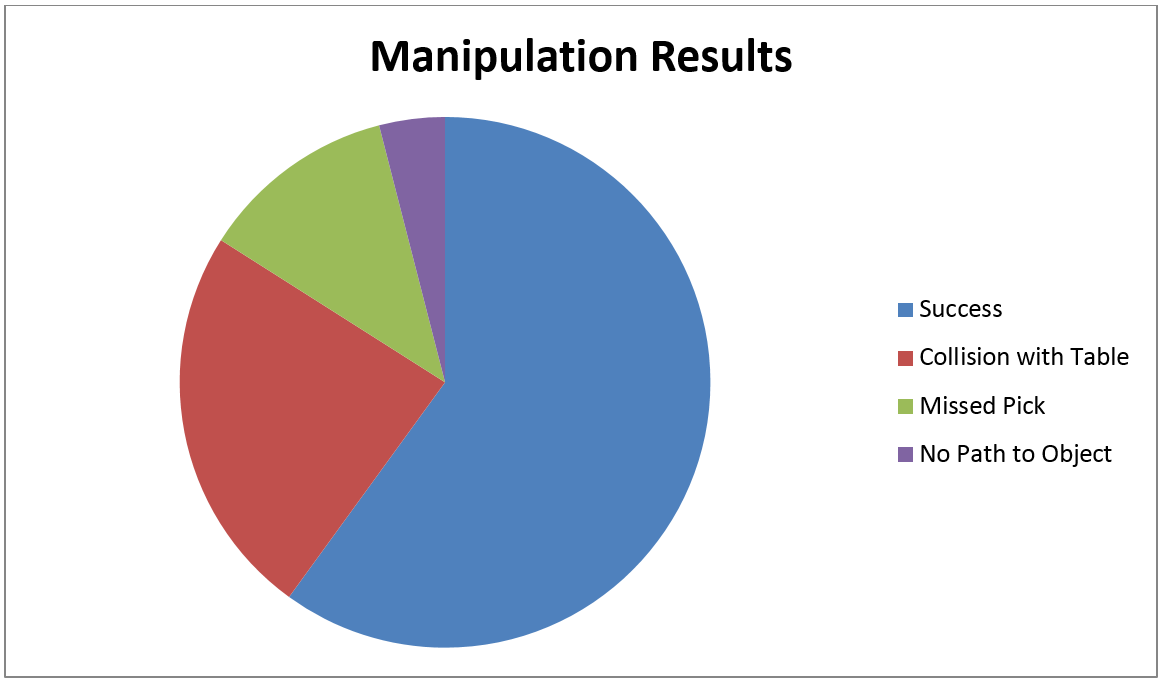
\includegraphics[width=6.0in]{manipulation_results}
\caption{Manipulation test results}
\label{fig:results-pie}
\end{figure}

Of the twenty-five trials, the robot completed the manipulation task
thirteen times. In three attempts, the gripper missed the object,
resulting in a failed pick. These failures can be attributed to the very
small clearance between the 5 cm object and the 5.3 cm gripper jaw. In
one of the trials (15), two objects were obscured from the Kinect by the
robot arm and the third was not reachable by the robot's arm. The most
common cause of failure was the robot gripper making contact with the
table. This problem caused six trials to fail. The ROS arm navigation
software used on the robot is configured to generate collision-free arm
trajectories, as described in Section \ref{arm-nav} above, but for an unknown
reason, it does not always do so. A proposed solution, using recently
released ROS software, is proposed in Chapter \ref{future-work} below.

\begin{longtable}[c]{lp{2.5cm}ll}
\caption{Results of object recognition and manipulation tests}
\label{tab:object-recognition}\tabularnewline
\endfirsthead
\toprule
\textbf{Trial} & \textbf{Objects Recognized} & \textbf{Pick Result} &
\textbf{Drop Result}\tabularnewline
\midrule
\endhead
1 & 3 & Success & Success\tabularnewline
2 & 3 & Success & Success\tabularnewline
3 & 3 & Success & Success\tabularnewline
4 & 2 & Success ( 3\textsuperscript{rd} attempt) &
Success\tabularnewline
5 & 2 & Missed (gripper nudges table) & Success (with no
object)\tabularnewline
6 & 2 & Success ( 2\textsuperscript{nd} attempt) &
Success\tabularnewline
7 & 3 & Success & Success\tabularnewline
8 & 4 & Success ( 2\textsuperscript{nd} attempt) &
Success\tabularnewline
9 & 2 & Success, insecure grip ( 3\textsuperscript{rd} attempt) &
Success (object fell)\tabularnewline
10 & 3 & Missed & Success (with no object)\tabularnewline
11 & 2 & Missed & Success (with no object)t\tabularnewline
12 & 2 & Success & Success\tabularnewline
13 & 2 & Missed (gripper nudges table) & Success (with no
object)\tabularnewline
14 & 2 & Success (2\textsuperscript{nd} attempt) &
Success\tabularnewline
15 & 1 & Cannot find a path to the object & N/A\tabularnewline
16 & 2 & Gripper hits table & N/A\tabularnewline
17 & 2 & Gripper hits table & N/A\tabularnewline
18 & 2 & Success & Success\tabularnewline
19 & 3 & Success & Success\tabularnewline
20 & 2 & Gripper hits table & N/A\tabularnewline
21 & 1 & Success, insecure grip ( 3\textsuperscript{rd} attempt) &
Success (object fell)\tabularnewline
22 & 2 & Success & Success (takes over 60 s)\tabularnewline
23 & 2 & Gripper hits table & N/A\tabularnewline
24 & 3 & Success & Success\tabularnewline
25 & 2 & Missed & Success (with no object)\tabularnewline
\bottomrule
\end{longtable}

Finally, these tests were combined into a single procedure that
simulates part of the task of retrieving an assembly kit from factory
inventory. The procedure is as follows:

\begin{enumerate}
\def\labelenumi{\arabic{enumi}.}
\item
  Beginning at one of two starting locations, drive to a predetermined
  location near a table a few meters away.
\item
  Locate at least one of three small manipulable objects on the table
  using the Kinect.
\item
  Lift one of the target objects from the table.
\item
  Place the target object in the onboard carrier bin.
\item
  Drive to the final destination.
\end{enumerate}

This task is meant to simulate the act of driving through a factory to a
shelf (represented by the table), picking up an item for a kit, and
delivering it to the assembly station. In an actual factory environment,
steps 1 through 4 would be performed repeatedly until every item in the
kit was retrieved.

The driving portions of the task test the drive base hardware and
software, including the localization and navigation systems. The object
recognition portion of the task tests the Kinect and the tabletop
perception software. The manipulation portions of the task test the arm
hardware and the arm navigation stack, including the inverse kinematic
solver, path planner, and collision environment monitor.

The task described was performed by the robot eight times. The robot
started from one of two locations, designated "left" and "right", which
were marked on the floor of the testing area. Between each trial, the
target objects were placed randomly within a designated area on the
table and the robot's localization software was reinitialized, with AMCL
seeded at the appropriate starting location. Of the eight trials
performed, seven were considered successful. Table \ref{table:validation} shows these
results.

\begin{longtable}[c]{@{}lp{3cm}p{2.5cm}p{7.5cm}@{}}
\caption{Validation Task Results}
\label{table:validation}\tabularnewline
\endfirsthead
\toprule
\textbf{Trial} & \textbf{Start
Position} & \textbf{Objects Recognized} & \textbf{Notes}\tabularnewline
\midrule
\endhead
1 & Left & 2 & Robot spins before settling into final
position\tabularnewline
2 & Left & 2 & Gripper brushes table and knocks over 1 object; robot
spins before settling into final position\tabularnewline
3 & Left & N/A & Robot approaches table, but get stuck in
spin\tabularnewline
4 & Left & 1 & Object recognition/pickup succeeds on fourth
attempt\tabularnewline
5 & Right & 1 & Low batteries prevent robot from aligning in final
position\tabularnewline
6 & Right & 2 &\tabularnewline
7 & Right & 1 & Low batteries prevent robot from aligning in final
position\tabularnewline
8 & Right & 3 & Robot spins before settling into final
position\tabularnewline
\bottomrule
\end{longtable}

Of the seven successful trials, most exhibit a similar behavior at the
end of the trial. The robot spins one or more times before settling into
the final position. This behavior (at the table, rather than the final
position) was also the cause of the single failed trial. The cause of
this behavior is unknown, but the drive base planners were observed to
be running slower than the desired rate due to the heavy load on the
PC's CPU. It is possible that this caused the robot to overshoot the
desired heading, causing it to perform a full rotation. Whereas the
robot eventually recovered from this problem at the final position, it
could not recover at the table because of the tight tolerance required
to approach so close to the table.

\section{Battery Performance}

Three tests were performed to determine the life of the battery. In each
test, the test process was run until the battery voltage reached 21.5
volts DC, which was considered the critical shutdown voltage. At this
point, each cell in the lead acid battery has been depleted to about 1.8
volts, or 90\% of its nominal voltage.

\begin{figure}[ht]
\centering
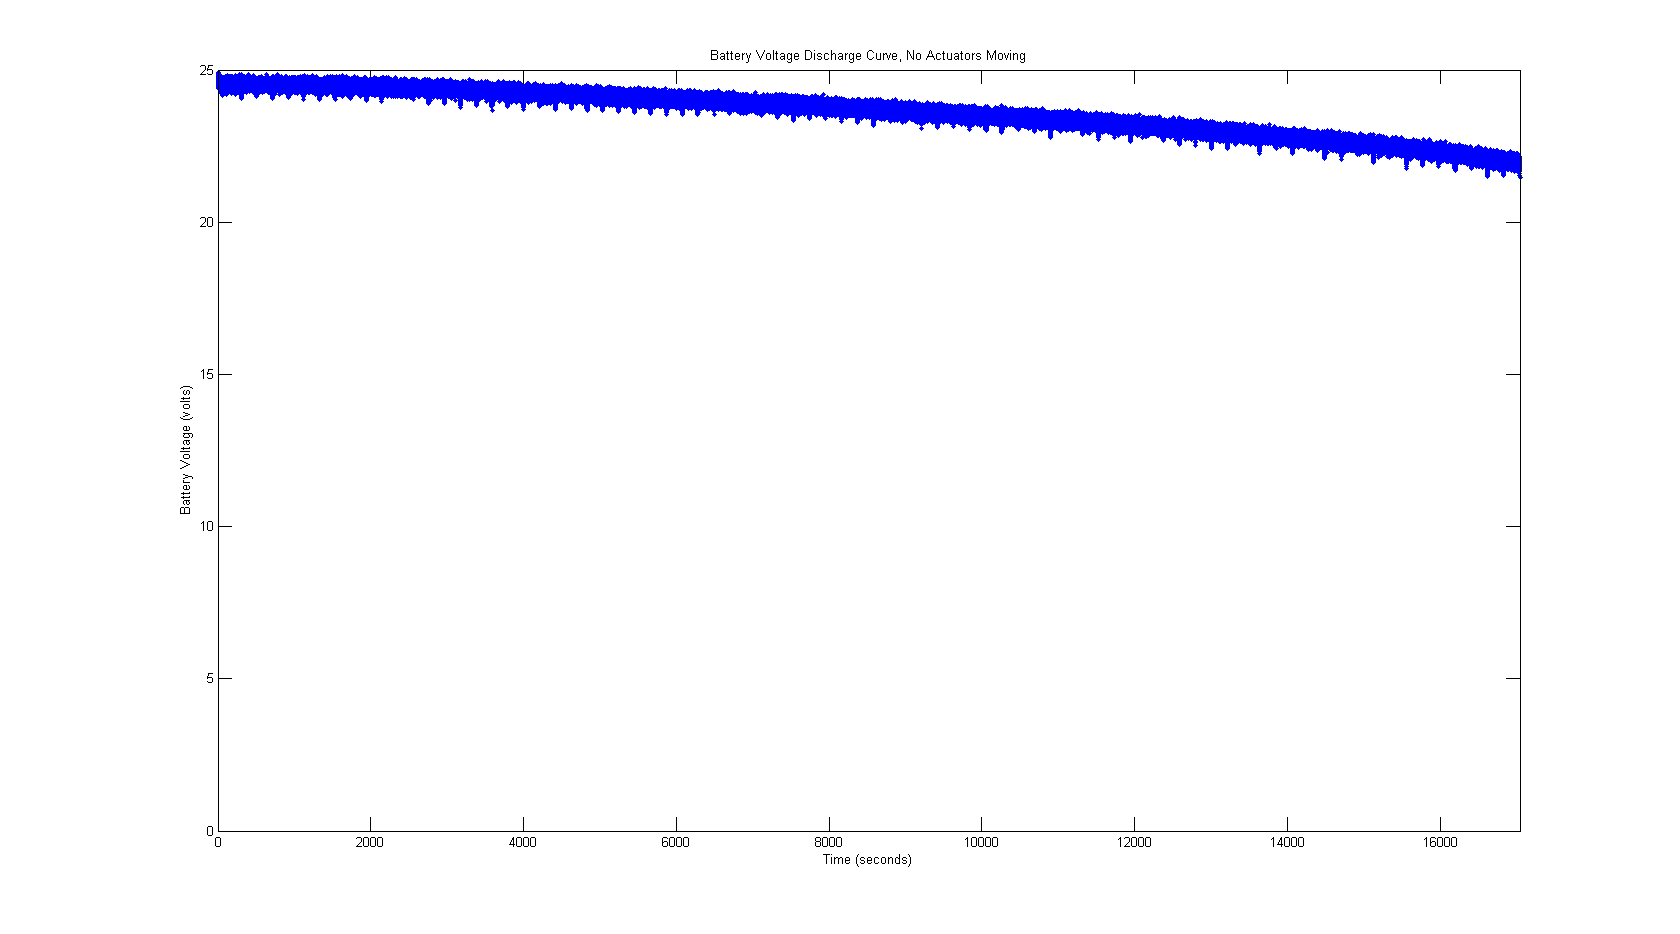
\includegraphics[width=6.0in]{discharge_idle}
\caption{Voltage curve during battery discharge test with actuators idle}
\label{fig:discharge-idle}
\end{figure}

In the first test, the robot's systems are all turned on, but the
actuators are disabled. In this idle test, the robot ran for 4 hours and
44 minutes before it hit the critical voltage.

In the second test, the robot was strapped to a platform with rollers,
and the drivetrain was exercised by commanding rotational velocities
that followed a sawtooth profile, increasing from the maximum negative
velocity to the maximum positive velocity, then resetting back to the
maximum negative velocity. In this test, the robot ran for 3 hours and
13 minutes before it hit the critical voltage.

\begin{figure}[ht]
\centering
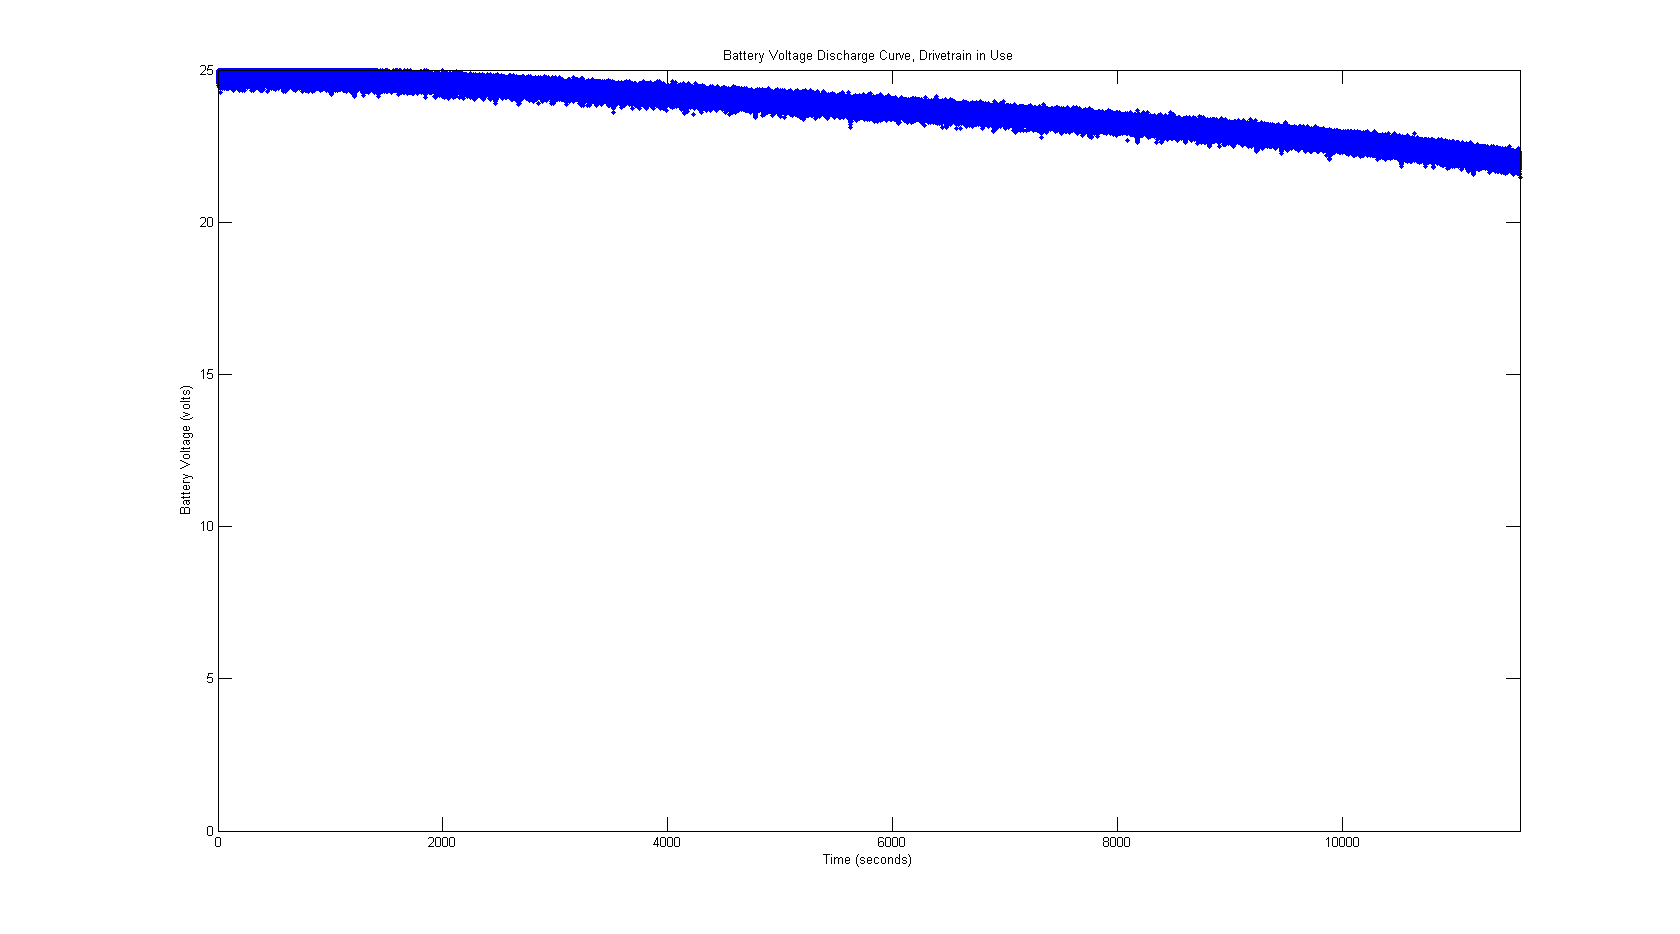
\includegraphics[width=6.0in]{discharge_drive}
\caption{Voltage curve during battery discharge test with drivetrain exercised}
\label{fig:discharge-drive}
\end{figure}

\begin{figure}[ht]
\centering
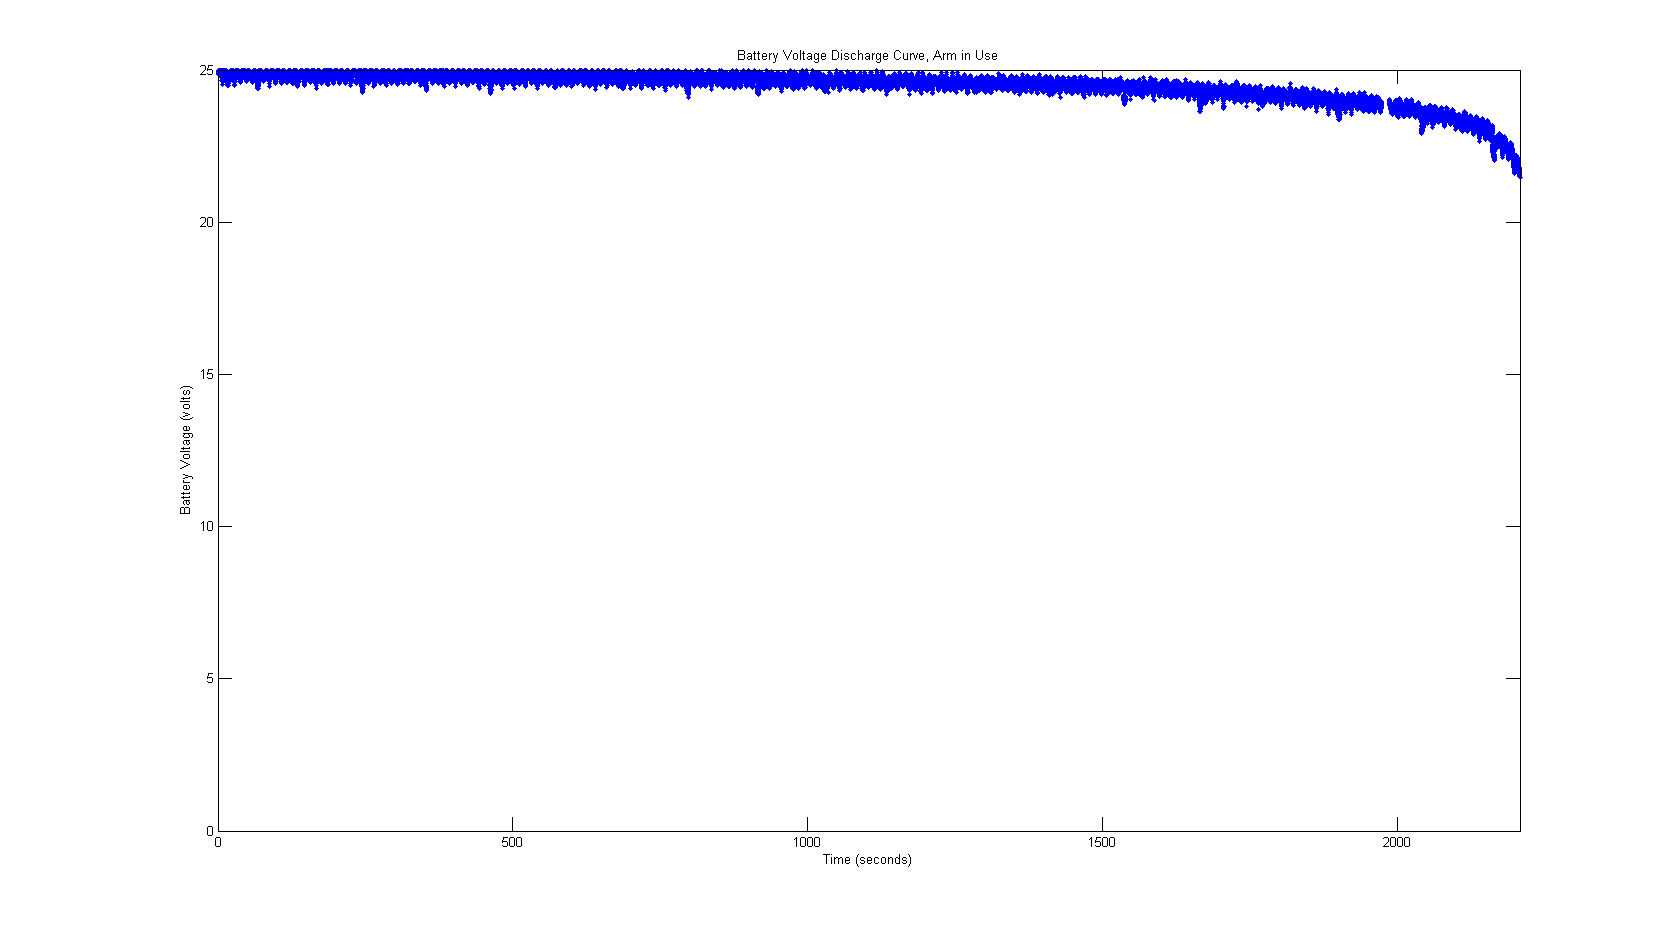
\includegraphics[width=6.0in]{discharge_arm}
\caption{Voltage curve during battery discharge test with arm exercised}
\label{fig:discharge-arm}
\end{figure}

In the third test, the drivetrain was disabled but the arm was commanded
to repeatedly execute trajectories between the stow position and the
position to drop an object in the bin. At the end of each trajectory,
the gripper was opened or closed. In this test, the robot ran for only
36 minutes. These results indicate that the arm consumes significantly
more power than other components of the robot.

These tests indicate that the robot could run in typical operation for
about one hour before its batteries are critically low.

\section{The Kinect}

\subsection{For Object Localization and Arm Planning}

A major part of the validation task depended on the Kinect as a sensor
for object segmentation and recognition. The Kinect point cloud was used
as the input to segmentation and localization nodes to determine the
location of manipulable objects on a table. Although the Kinect has been
shown to have some warping{[}32{]}, it proved adequate to recognize the
small cylindrical objects used for the validation task. Two different
Kinects were tested on this robot. The first Kinect used was improperly
calibrated, and its color data was very badly registered to its depth
data. It is unknown whether this is caused by a factory defect or damage
during use. The second Kinect tested did not exhibit these problems and
was successfully used to localize objects in the validation task.

\subsection{For Reading QR Codes}

The Kinect's RGB camera captures video at VGA resolution (640 by 480
pixels). Experiments with reading QR codes showed that a Kinect did not
have sufficient resolution to read a tag, even when the tag filled the
entire field of view of the Kinect. This means that in order for the
Kinect to be useful for recognition of tagged ``smart'' payloads, it
must be paired with (and calibrated to) an external camera with a higher
resolution sensor.

\chapter{Conclusion}

The lack of cheap, robust mobile manipulators has prevented
manufacturers from adopting them and has hampered research into mobile
manipulation. ABBY, being both cheap and robust, fills the needs of both
groups. With a total component cost less than \$40,000, this platform is
significantly cheaper than existing mobile manipulation platforms. This
savings in cost was in large part due to the use of mass-produced
hardware components. The hardware platform is constructed of industrial
and commercial components. These components have been rigorously tested
by their manufacturers and in the field. As a result, the hardware is
more durable than experimental ``research-grade'' hardware, which is not
subject to the quality controls of mass-produced products. These
hardware components were successfully integrated into a system capable
of traversing indoor environments and manipulating small objects.

In addition to a robust hardware platform, existing software from the
ROS community was integrated to create a capable robot. ABBY is able to
navigate indoor environments with \emph{a priori} maps using a
combination of relative and global localization and a ROS-standard
planner. Using ROS software adapted to this platform, ABBY can locate
objects on a table using a Kinect camera. A software driver for ABB
industrial robotic arms was created specifically for this project and
contributed to the ROS Industrial project. Using this software, ABBY can
pick up recognized objects and store them in an onboard carrying bin.
The software on ABBY is modular, using existing ROS frameworks and APIs
wherever possible. The use of a modular software system will enable
future researchers to easily augment the system with new experimental
software.

Overall, the robot shows promising initial results. In sixteen trials of
the mobile base, fifteen were complete successes. Of twenty-five trials
of the manipulation system, fifteen were successes. The limited range of
the gripper calls for precise object localization, which was nonetheless
achieved with the Kinect in the majority of trials. The biggest problem
with the manipulation system was unreliable collision checking.
Development of collision checking software was beyond the scope of this
project, and this is an area of future research. In combined mobile
manipulation trials, the robot performed its task perfectly in seven out
of eight trials. These results show that the robot's hardware and
software systems are reliable enough to make it a useful research
platform, demonstrating that a mobile manipulator can be created for
much lower cost than currently available platforms.

This robot was designed for experiments with kitting operations in a
factory environment. However, the platform is useful for other
applications as well. Researchers at other institutions have used mobile
manipulators for household tasks, and this platform could be used for
similar research. This research could also dovetail with previous work
at Case into assistive robots for the disabled. By providing a low-cost
platform for mobile manipulation research, this robot enables
researchers to tackle these and other problems without the significant
expense of other mobile manipulators.

This robot, with upgrades to its end effector, would also be an
effective mobile manufacturing platform. Rather than having to build and
rebuild a fixed manufacturing cell for each change in production
requirements, industrial engineers could design rapidly reconfigurable
assembly lines composed of one or more mobile manipulators. These
systems would also allow rapid set-up of small manufacturing operations
at new manufacturing sites and remote locations such as construction
sites or in space.

\chapter{Future Work}
\label{future-work}

Although this platform is now functional and useful for research, there
are several areas in which future researchers could improve it.

The biggest problem with the manipulation subsystem is that the ROS arm
navigation software sometimes generates trajectories that result in
collisions with furniture in the robot's environment. The cause of this
problem is unknown. Future researchers should evaluate alternative
ROS-compatible collision checkers.

The current power system only allows about one hour of operation before
recharging the batteries. The ability to charge or change the batteries
autonomously would make the robot more useful.

There are two promising avenues of exploration to reduce the cost of the
platform. The cRIO and auxiliary hardware used to control the mobile
base (breakout boards and speed controllers) account for over 10\% of
the overall system cost. Future researchers should explore newer, more
affordable alternatives to reduce the cost of the system without
compromising its capabilities. The SICK LIDAR accounts for over 15\% of
the overall system cost. Future researchers should evaluate other
ranging sensors to determine if there is a more affordable alternative
that is sufficiently accurate and robust for this platform.

Evaluation and integration of more sensors could allow the robot to
perform more functions than it can now. The Kinect is a low-resolution
(VGA) camera, and one of the key future goals of this project is to be
able to identify manipulable objects from bar codes or QR codes. A
higher resolution camera (perhaps mounted on the robot's manipulator)
could be used to examine objects to be picked up. Because the robot has
no rear-facing sensors, it cannot safely back up, and SLAM algorithms
fail when the robot drives through doorways. Adding rear-facing sensors
would allow the robot to safely back up and might also solve the
problems that prevented the use of SLAM for absolute localization.

The two-position parallel plate gripper used for this project was simple
and readily available, but it limits the robot to being able to
manipulate boxes in a limited range of sizes. Future researchers should
explore different types of grippers and evaluate their cost
effectiveness and performance in this robot's intended application.

Over the course of the project, several problems were identified with
ROS stability. For ROS software to be a viable option in an industrial
environment, it must be meticulously tested and shown to be robust,
secure, and safe. Currently, most software outside of the ROS core does
not meet these requirements. Testing more ROS packages and improving
their stability would be a boon to the open source robotics community
and to the industrial robotics industry.

As described above, the current emergency stop system is incomplete and
relies on a tethered emergency stop button. A revised emergency stop
design, described in Appendix 2, was created as part of this thesis, but
has not yet been constructed and installed on the platform.

As described above, the robot currently operates at low speed so that a
reflexive speed limiting system is not necessary. Adding reflexive speed
limiting to the robot would allow high speed operation without
compromising safety. Some proposed speed limiting systems are described
in Appendix 3.

\appendix

\chapter{Bill of Materials}

\begin{longtable}[c]{@{}ll@{}}
\caption{Bill of Materials}
\label{tab:bom}\tabularnewline
\endfirsthead
\toprule
\textbf{Item} & \textbf{Cost}\tabularnewline
\midrule
\endhead
Wheelchair Base & \$3000\tabularnewline
Batteries & \$400\tabularnewline
Chassis Frame Materials & \$1000\tabularnewline
LIDAR & \$6000\tabularnewline
IRB-120/IRC5 & \$23000\tabularnewline
\vtop{\hbox{\strut cRIO 9074}\hbox{\strut + 9403 DIO
module}\hbox{\strut +9401 DIO module}\hbox{\strut + 9201 analog input
module}} & \$4150\tabularnewline
PC

\vtop{\hbox{\strut Case}\hbox{\strut Power Supply}\hbox{\strut Solid
State Hard
Drive}\hbox{\strut Motherboard}\hbox{\strut Processor}\hbox{\strut RAM}}

Total &
\vtop{\hbox{\strut \$65}\hbox{\strut \$90}\hbox{\strut \$50}\hbox{\strut \$70}\hbox{\strut \$230}\hbox{\strut \$42}}

\$547\tabularnewline
Kinect & \$150\tabularnewline
Grayhill Encoder (4) & \$320\tabularnewline
13.8 v Regulator & \$81\tabularnewline
I/O Breakout Board & \$45\tabularnewline
Emergency Stop System & \$160\tabularnewline
AC Inverter & \$322\tabularnewline
Sabertooth 2x50 & \$250\tabularnewline
Compressor & \$250\tabularnewline
Network Equipment & \$40\tabularnewline
RS-422 -- USB converter & \$80\tabularnewline
Arduino & \$30\tabularnewline
Miscellaneous Electrical Components & \$50\tabularnewline
\textbf{Total} & \$1778.00\tabularnewline
\bottomrule
\end{longtable}

\chapter{Revised Emergency Stop Design}

A revised version of the emergency stop circuit was designed and
portions of it prototyped, but it has not been tested. This version
should fix the problems discovered in the first version of the emergency
stop.

\begin{figure}[ht]
\centering
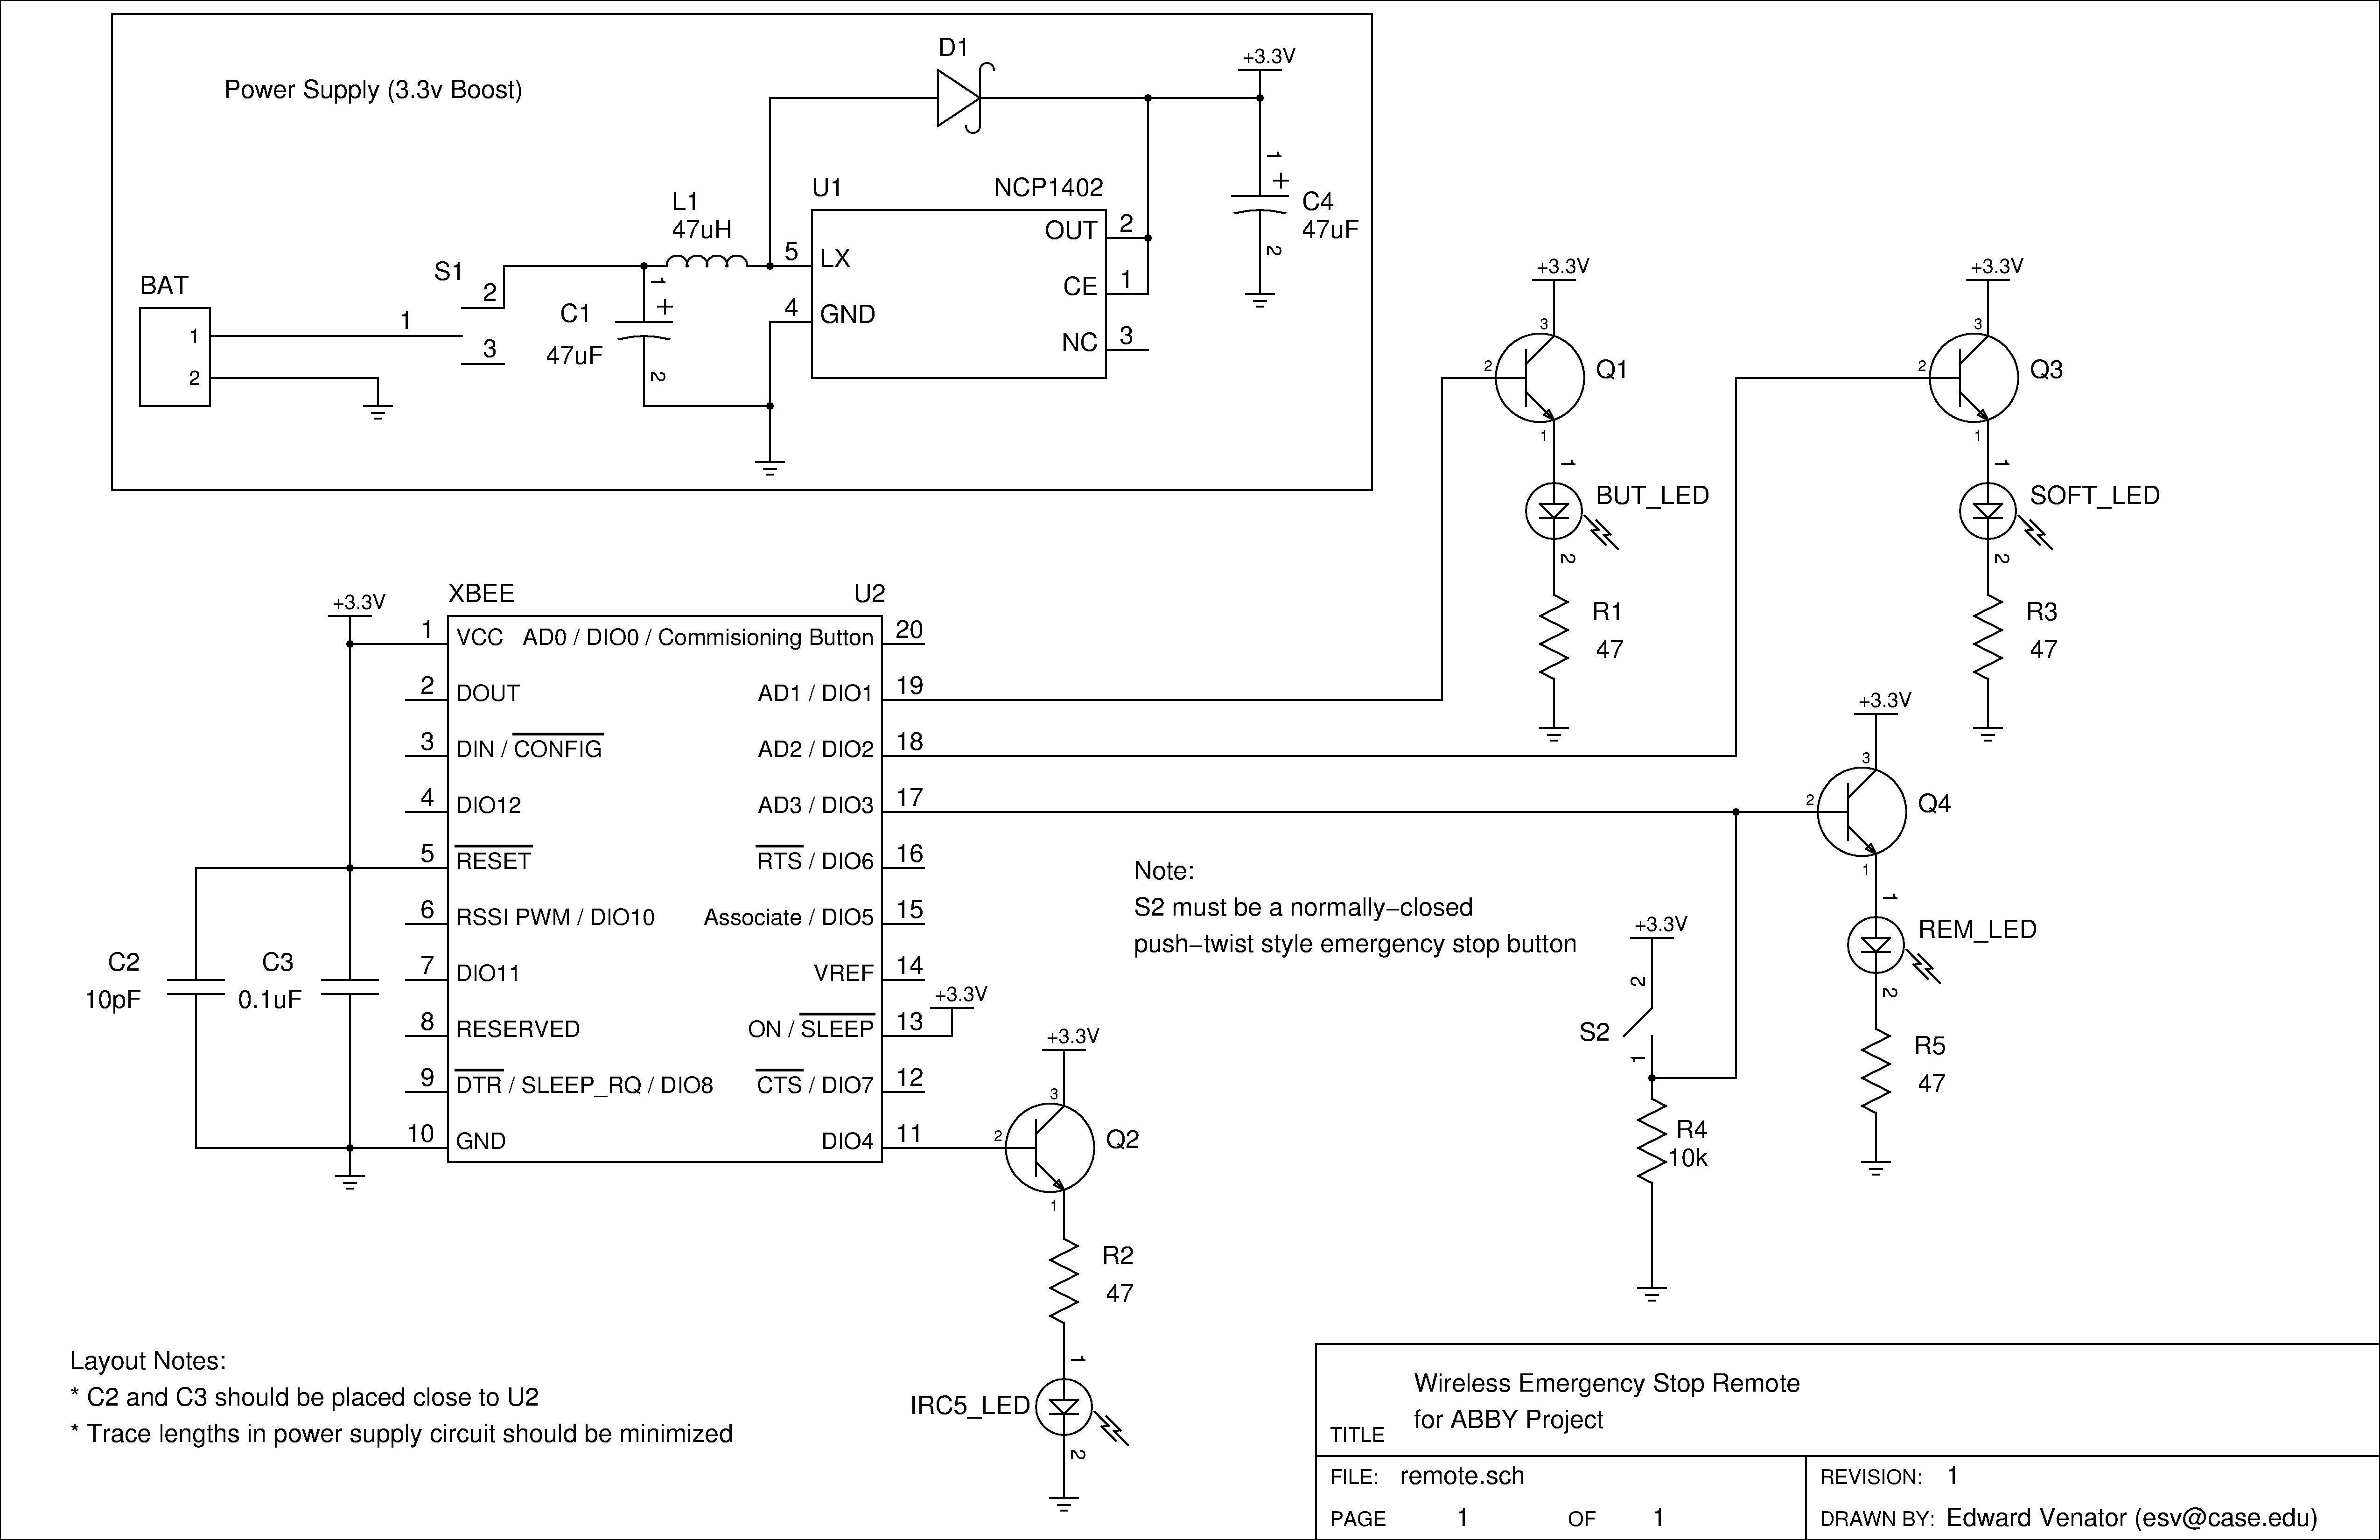
\includegraphics[width=6.0in]{estop_remote_revised}
\caption{Revised emergency stop remote circuit.}
\label{fig:estop-remote-revised}
\end{figure}

To allow the system to stop the IRC5, the optoisolator on the output of
the emergency stop circuit was replaced with a relay module, which will
more reliably switch the General Stop input of the IRC5. To complete
integration with the IRC5, the RAPID software must be modified to output
the current General Stop state to a GPIO, which should be connected to
the IRC5 input of the emergency stop circuit.

\begin{figure}[ht]
\centering
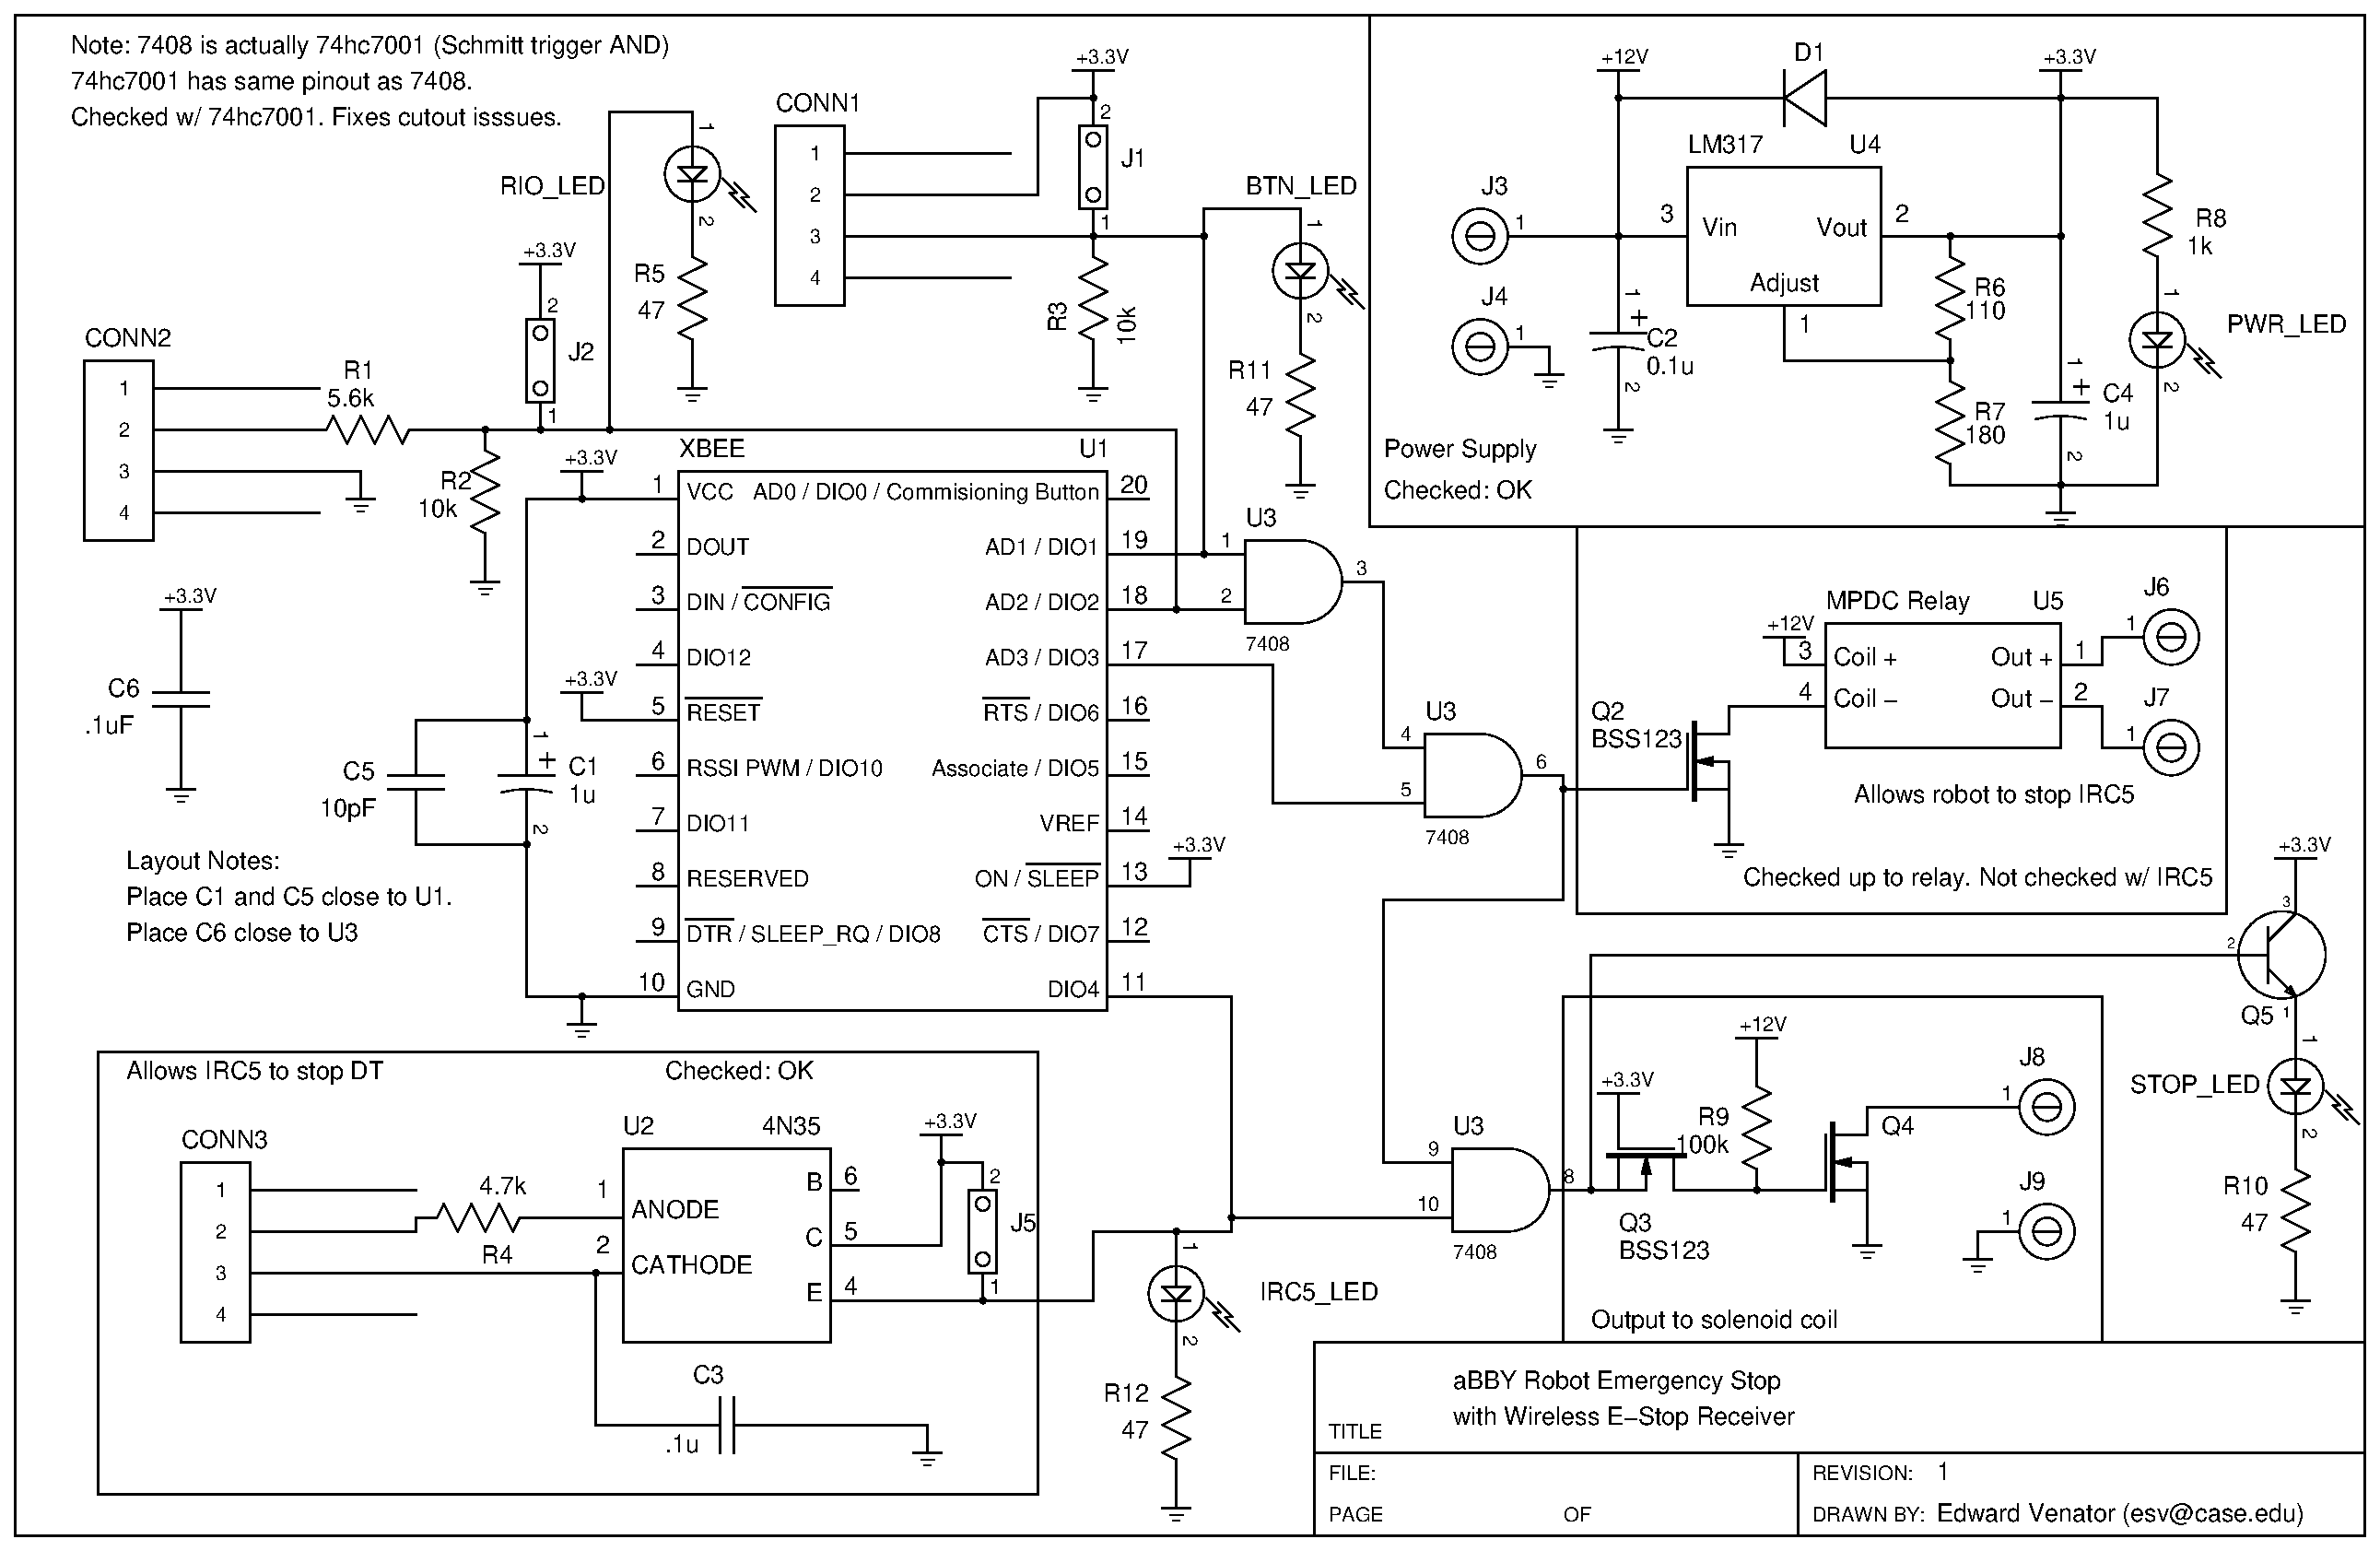
\includegraphics[width=6.0in]{estop_receiver_revised}
\caption{Revised emergency stop receiver/aggregator circuit.}
\label{fig:estop-receiver-revised}
\end{figure}

To solve the wireless communication issues, the power supply in the
remote was replaced with a 3.3 volt regulated boost supply, which should
be much more reliable, and bypass capacitors were added to the power
rails of the XBee modules on both the remote and the emergency stop
circuit. Testing has shown that the XBee modules are reliable when a
sufficiently clean and reliable DC supply is available to power them.

In addition to solving the problems described above, some small changes
were made to improve the circuit. To reduce the power consumption of the
emergency stop circuit and reduce the heat produced by the onboard power
regulator, the Darlington transistor used to switch the coil of the
drivebase enable solenoid was replaced with a MOSFET circuit that
performs the same function. To make the system easier to use and more
reliable, the momentary switch and latch used on the previous version
was replaced with a twist-lock style emergency stop switch.

Although this system has not been constructed, its constituent parts
have been tested individually. The MOSFET switching circuit has been
confirmed to work with a resistive load equivalent to the coil
resistance of the solenoid used to switch the drive base power rail. The
power supply circuit in the remote has been tested and provides a
reliable 3.3 volt power supply from a pair of AA batteries. The use of a
relay instead of a transistor to control the General Stop input is in
line with recommendations from ABB's documentation, and the relay used
meets the requirements. If the necessary components can be acquired for
this emergency stop circuit, it should be able to meet all of the
requirements described above.

\chapter{Reflexive Collision Avoidance}

As described in Section \ref{reflexive-avoidance}, ABBY is slow enough that it can be operated
safely without a reflexive speed limiting system. This appendix
describes proposed speed limiting systems to allow the robot to be
operated more quickly.

\section{Reflexive Halt Methods for Mobile Bases}

ABBY's local planner will not allow for collisions with obstacles seen
by the LIDAR, and it updates velocity commands at 12 Hz. Although this
is sufficiently safe for testing, a more robust solution would be
necessary in an industrial setting. Mobile robots often implement a
reflexive halt as shown in Algorithm \ref{alg:reflexive-halt}. For example,
if a measurement source such as a LIDAR reports that there is an obstacle in 
front of the robot at close range, the robot's velocity would be limited to 
turning and reversing. This approach is effective, but can cause difficulties 
in navigating tight areas, where there may be enough space for a robot to
navigate through obstacles if it does so carefully.

\begin{algorithm}
\caption{A simple reflexive halt
algorithm. If an obstacle is close to the robot, the robot is prevented
from approaching closer.}
\label{alg:reflexive-halt}
\begin{algorithmic}
\STATE \textbf{Given:} Sensor measurements $M$
\FORALL{measurement $m$ in $M$}
  \IF{dangerous($m$)}
    \STATE prevent motion in direction of $m$
  \ENDIF
\ENDFOR
\end{algorithmic}
\end{algorithm}

Another approach to reflexive halting was described by Chad Rockey in
his masters thesis \cite{rockey}. This approach, called Reflexive Avoidance
Plus, was developed for a smart wheelchair, which must operate in
crowded areas around people. Reflexive Avoidance Plus uses velocity
limiting rather than preventing motion altogether. When a sensor detects
an obstacle in the robot's path, it limits the maximum velocity in that
direction using a scaling function based on the distance of the obstacle
from the robot. This approach prevents the robot from colliding with an
obstacle (the maximum velocity is zero below a certain threshold
distance), but allows low speed progress toward an obstacle. Because the
robot approaches the obstacle at lower speed, it can safely get closer
to obstacles.

Since the Reflexive Avoidance Plus method described by Rockey was
implemented on a robotic platform of similar size and speed to this
robot, it would be a good candidate for this robot. However, there is
some work still to be done to adapt the code, which was designed
specifically for the wheelchair, to ABBY.

\section{Reflexive Halting for Manipulators}

In addition to the mobile base, ABBY's robotic arm poses a risk for
collisions. In industrial situations, manipulators are kept inside
safety cages to prevent people from interfering with them or getting
injured. A safety cage is not a possibility for a mobile manipulator, so
another solution is necessary. A reflexive halt for the manipulator
allows it to operate safely in the presence of people and obstacles
without a safety cage.

Like the mobile base planner, the planner for the arm generates
collision-free paths. However, the planner for the arm does not replan
at all once it commits to a trajectory. The trajectory is generated and
sent to the IRC5 for execution, and then ROS waits for the trajectory to
be executed. If something enters the path of the trajectory, the robot
does not alter the current trajectory. This makes the robot unsafe to
operate around humans above a certain joint speed.

Rethink Robotics, with their robot Baxter \cite{rethink}, solved the problem of
operating an industrial robot without a safety cage with a mechanical
and software solution that relied on force feedback and serial-elastic
actuators. Because all of Baxter's joints are elastic and its arms are
so light, it can safely collide with people and obstacles. It also uses
force feedback in its joints to detect these collisions and become
passive, allowing people to push it around. Because ABBY's robotic arm
does not have serial elastic actuators or force feedback in the joints,
this solution is not possible.

Using the Kinect sensor, it would be possible to implement one of
several possible reflexive collision avoidance methods on ABBY. One
method would be to halt arm motion when an obstacle enters the arm's
work envelope and suspend arm motion until the obstacle leaves the work
envelope. Although this is arguably the safest solution, it can cause
the robot to become stuck in the stopped state. If an inanimate obstacle
is brought into the robot's work envelope and left there, the robot will
never re-enable the arm.

To resolve this problem, the reflexive halt behavior can be augmented as
shown in Algorithm \ref{alg:reflexive-manip}. In this algorithm, the currently planned path is
repeatedly checked for dangerously close objects (such as people) until
execution is completed. If an object enters the dangerous area, the
robot stops execution of the trajectory and waits. If the obstacle
leaves the area before a timeout is reached, the robot resumes execution
of the trajectory. If the obstacle does not move, the robot will attempt
to retry planning to move around the obstacle to accomplish its goal.
This reflexive halt algorithm has two advantages over the naive
algorithm described in the previous paragraph. First, it does not stop
for obstacles that enter the work envelope but do not interfere with the
planned motion. This allows humans to work alongside the robot and
interact with it by giving it objects or taking objects from it. Second,
it will plan around stationary objects that enter the work envelope,
allowing a person to leave an object in the work envelope without
stalling the robot.

\begin{algorithm}
\caption{An algorithm for reflexive halting for a mobile manipulator.
If an obstacle enters the manipulation path, the robot waits, then 
replans.}
\label{alg:reflexive-manip}
\begin{algorithmic}
\STATE \textbf{Given:} Current Plan $P$, Measurements $M$
\FORALL{state $s$ in $P$}
  \FORALL{measurement $m$ in $M$}
    \IF{dangerous($m$, $s$)}
      \STATE halt
      \STATE wait for obstacle to move or replan
    \ENDIF
  \ENDFOR
\ENDFOR
\end{algorithmic}
\end{algorithm}

The National Institute for Standards and Tests (NIST) has developed an
algorithm to determine a safe separation distance $S$ for a human to
approach a robot. This is described in Equation \ref{eq:NIST} below, where
$K_H$ is the speed of a moving human, $K_R$ is
the speed of the robot, $T_R$ is the reaction time of the
human, $T_B$ is the braking time of the robot, $B$ is the
robot braking distance, and $C$ is a distance to account for measurement
uncertainty \cite{shackleford}.

\begin{equation}
\label{eq:NIST}
S = K_{H} * ( T_{R} + T_{B} ) + K_{R} * T_{R} + B + C
\end{equation}

NIST researchers used this equation, LIDAR scanners, and a Kalman filter
to track humans moving through the robot's work envelope and determine
whether a human had entered a danger zone around the robot (if the
distance from the robot to the human is less than $S$). This method
completes Algorithm \ref{alg:reflexive-manip} by filling in the dangerous() function. In order
to implement this algorithm on ABBY, parameters $B$ and $C$ would first have
to be determined for this platform. Then, the algorithm would have to be
written as a ROS node and tested on this robot.

\backmatter

\bibliographystyle{IEEEtran}
\bibliography{thesis}

\end{document}
